\documentclass[4pt]{beamer} % 16:9 widescreen layout

% --- Theme Selection ---
\usetheme{Madrid}        % Clean, professional layout with a footer
\usecolortheme{whale}    % Deep blue color scheme
\usepackage{pdfpages}
\usepackage{geometry}
\geometry{papersize={128mm,165.65mm}}

% --- Presentation Metadata ---
\title[Short Title]{Your Presentation Title}
\subtitle{Optional Subtitle}
\author[]{Your Name}
\institute[IIT Bombay]{University / Company Name}
\date{\today}

\begin{document}

% Slide 1: Title Page


% Slide 2: Table of Contents (Generated automatically from \section tags)
\begin{frame}{Index}
    \tableofcontents
\end{frame}

\section{Introduction and Random Variables}


% Needs \usepackage{pdfpages} in the preamble

\subsection{Introduction}
{
\setbeamercolor{background canvas}{bg=} 
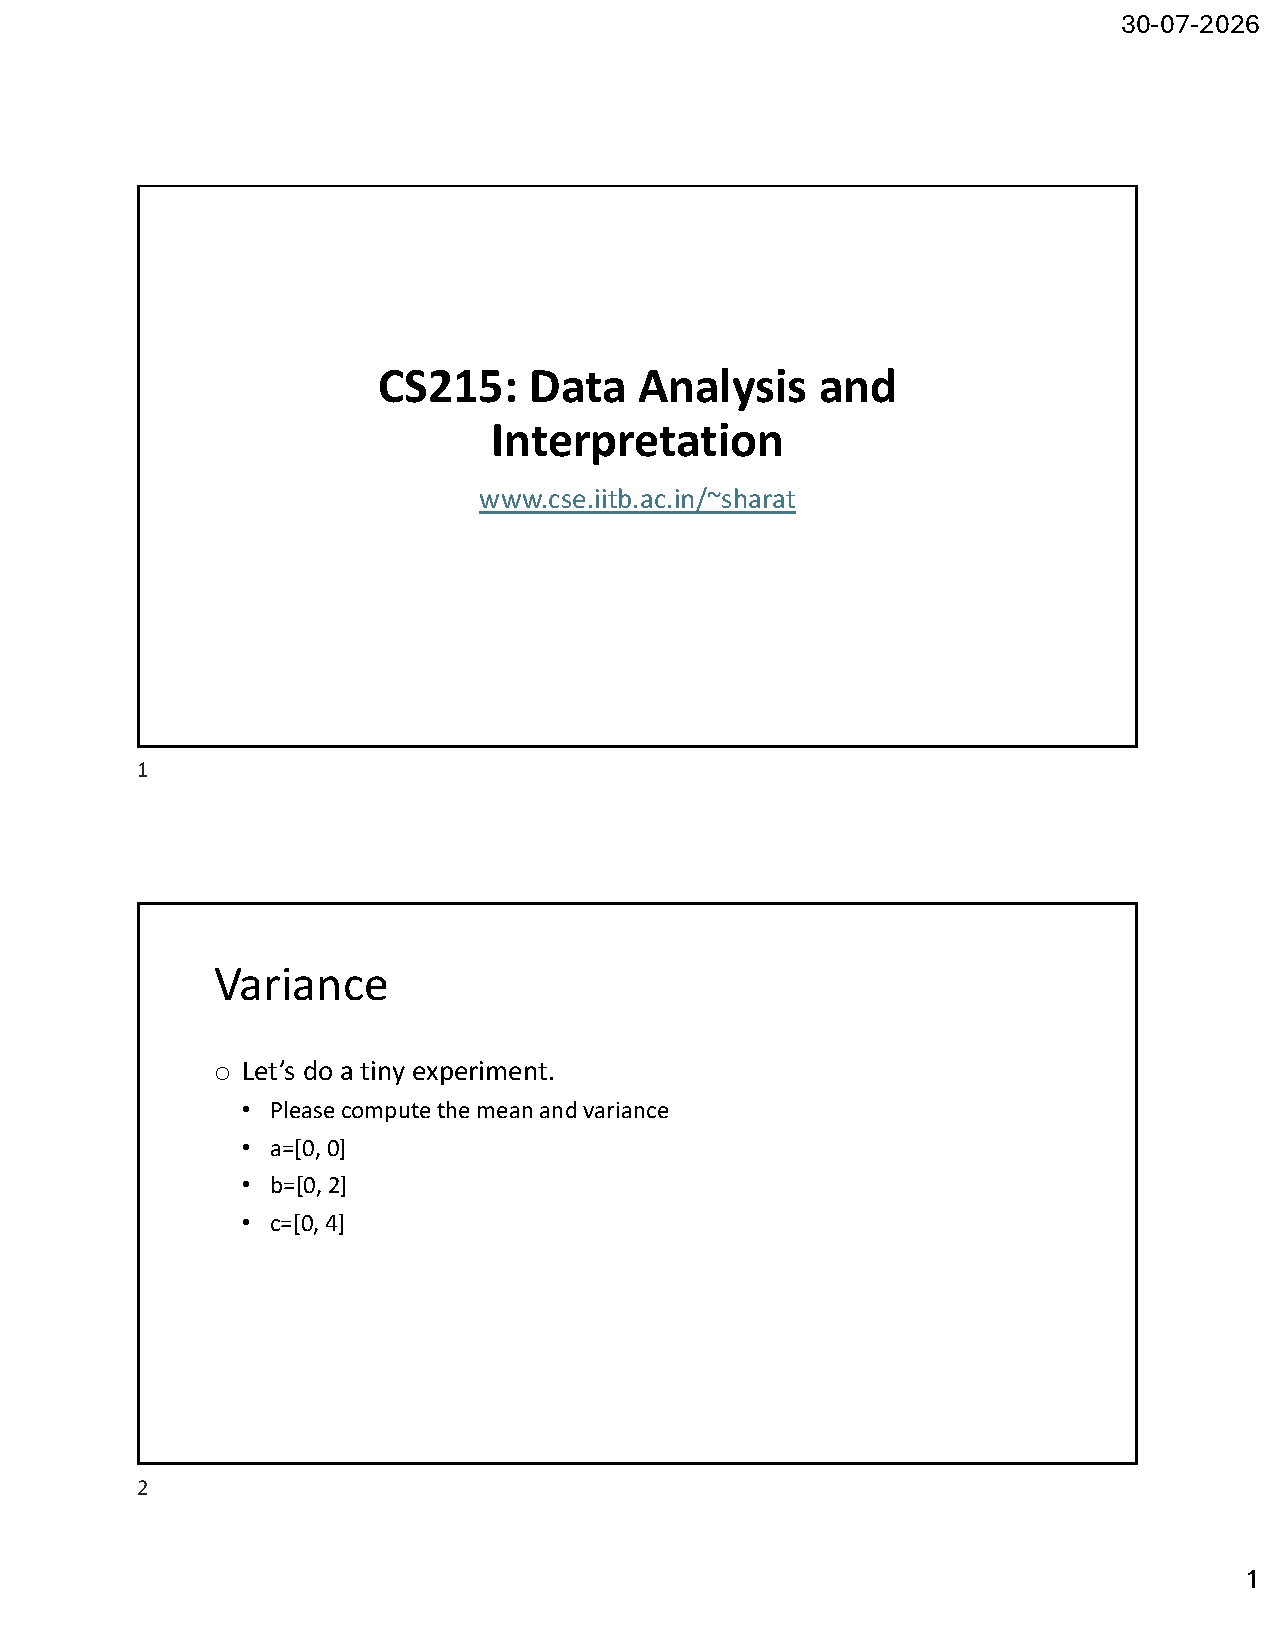
\includepdf[pages=-]{Lec01.pdf}
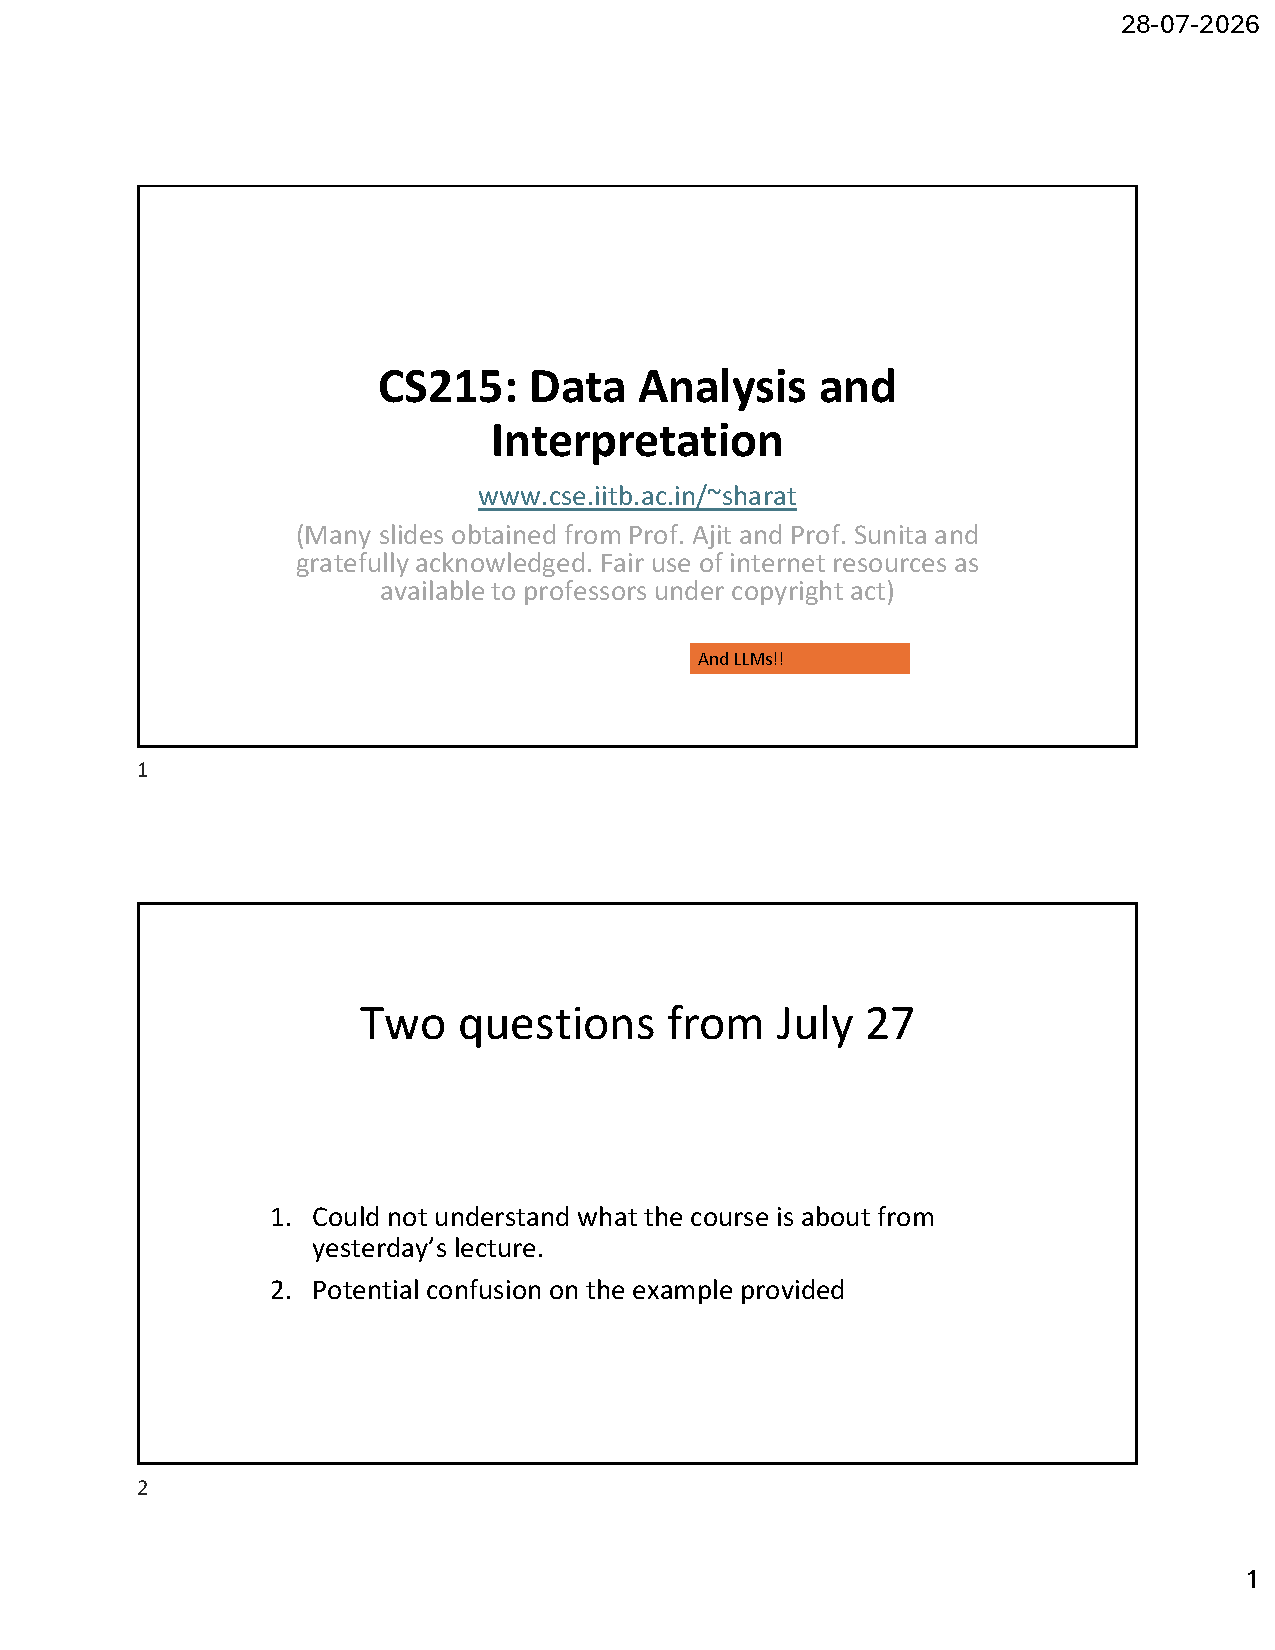
\includepdf[pages=-]{Lec02.pdf}
}


\subsection{Random Variables}
{
\setbeamercolor{background canvas}{bg=} 
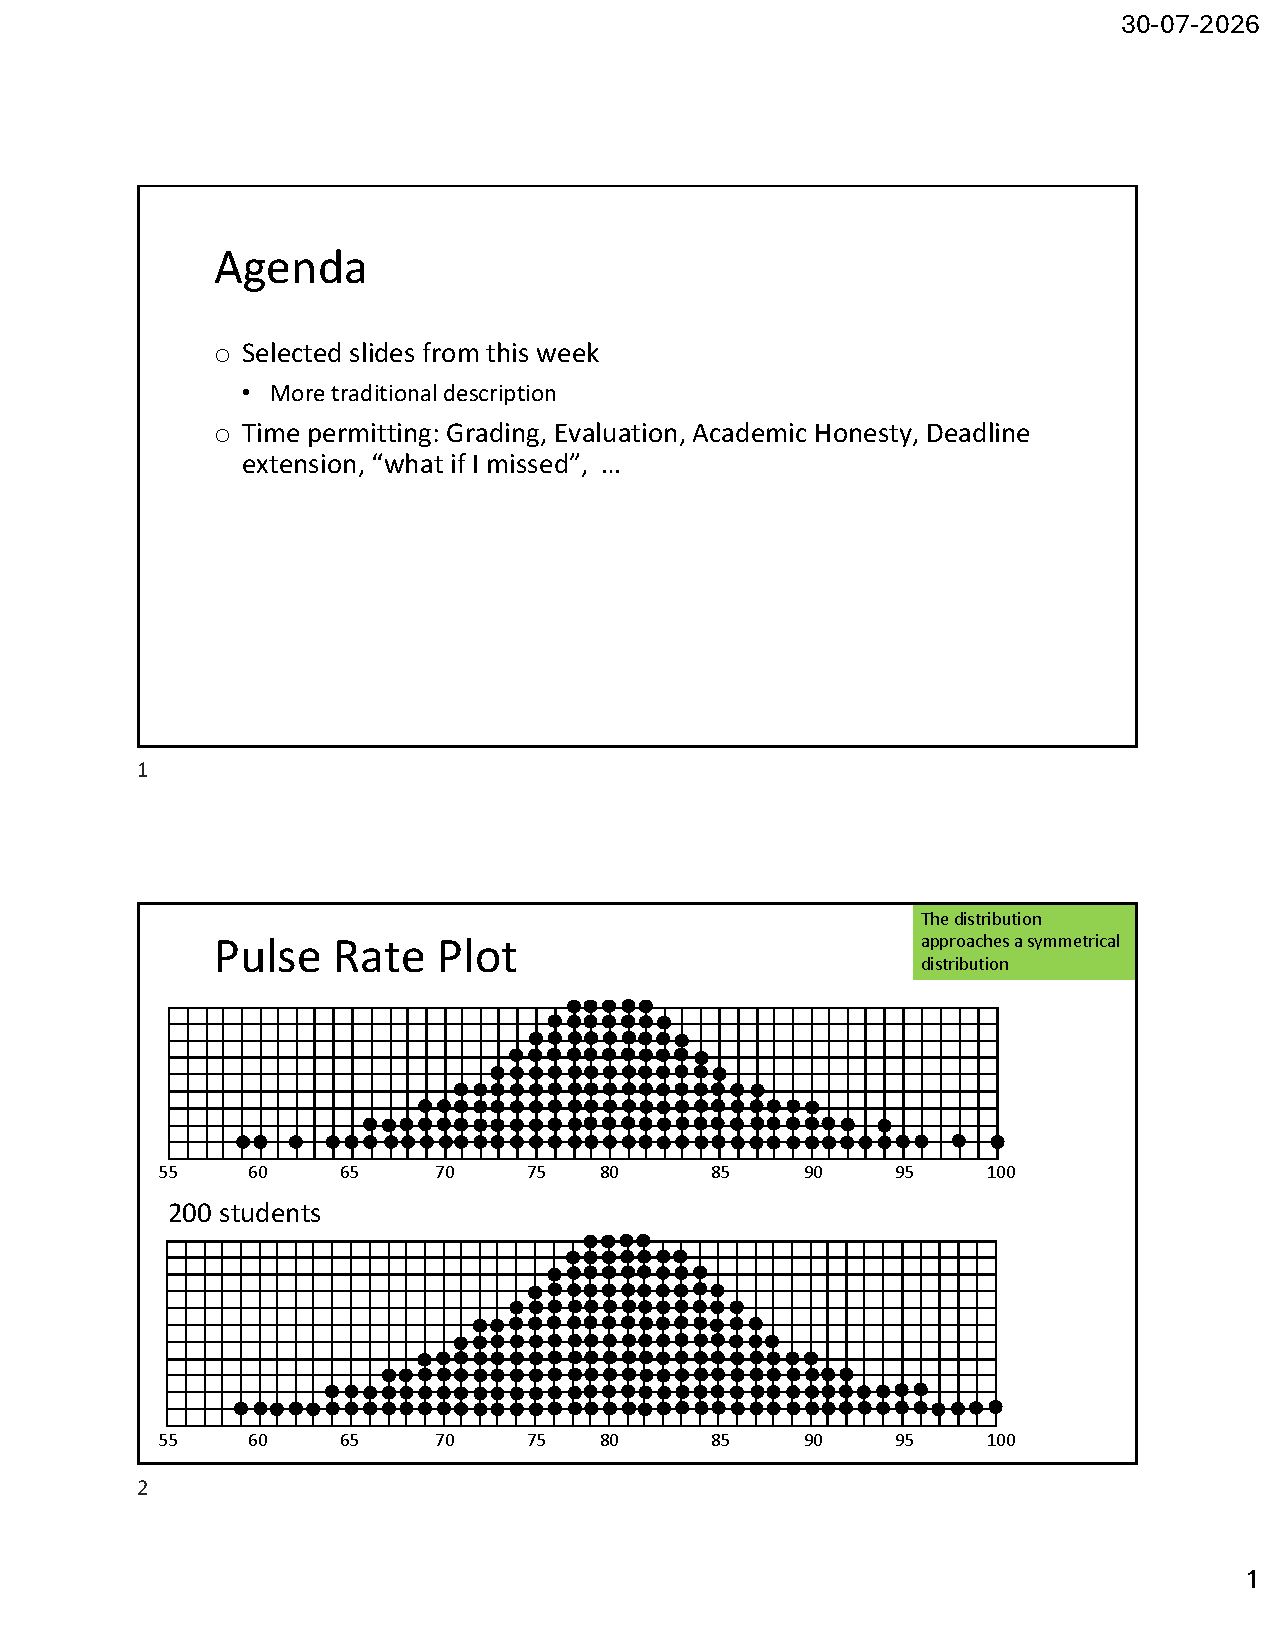
\includepdf[pages=-]{Lec03.pdf}
}

\subsection{Expectation and Variance of Random Variables}
{
\setbeamercolor{background canvas}{bg=} 
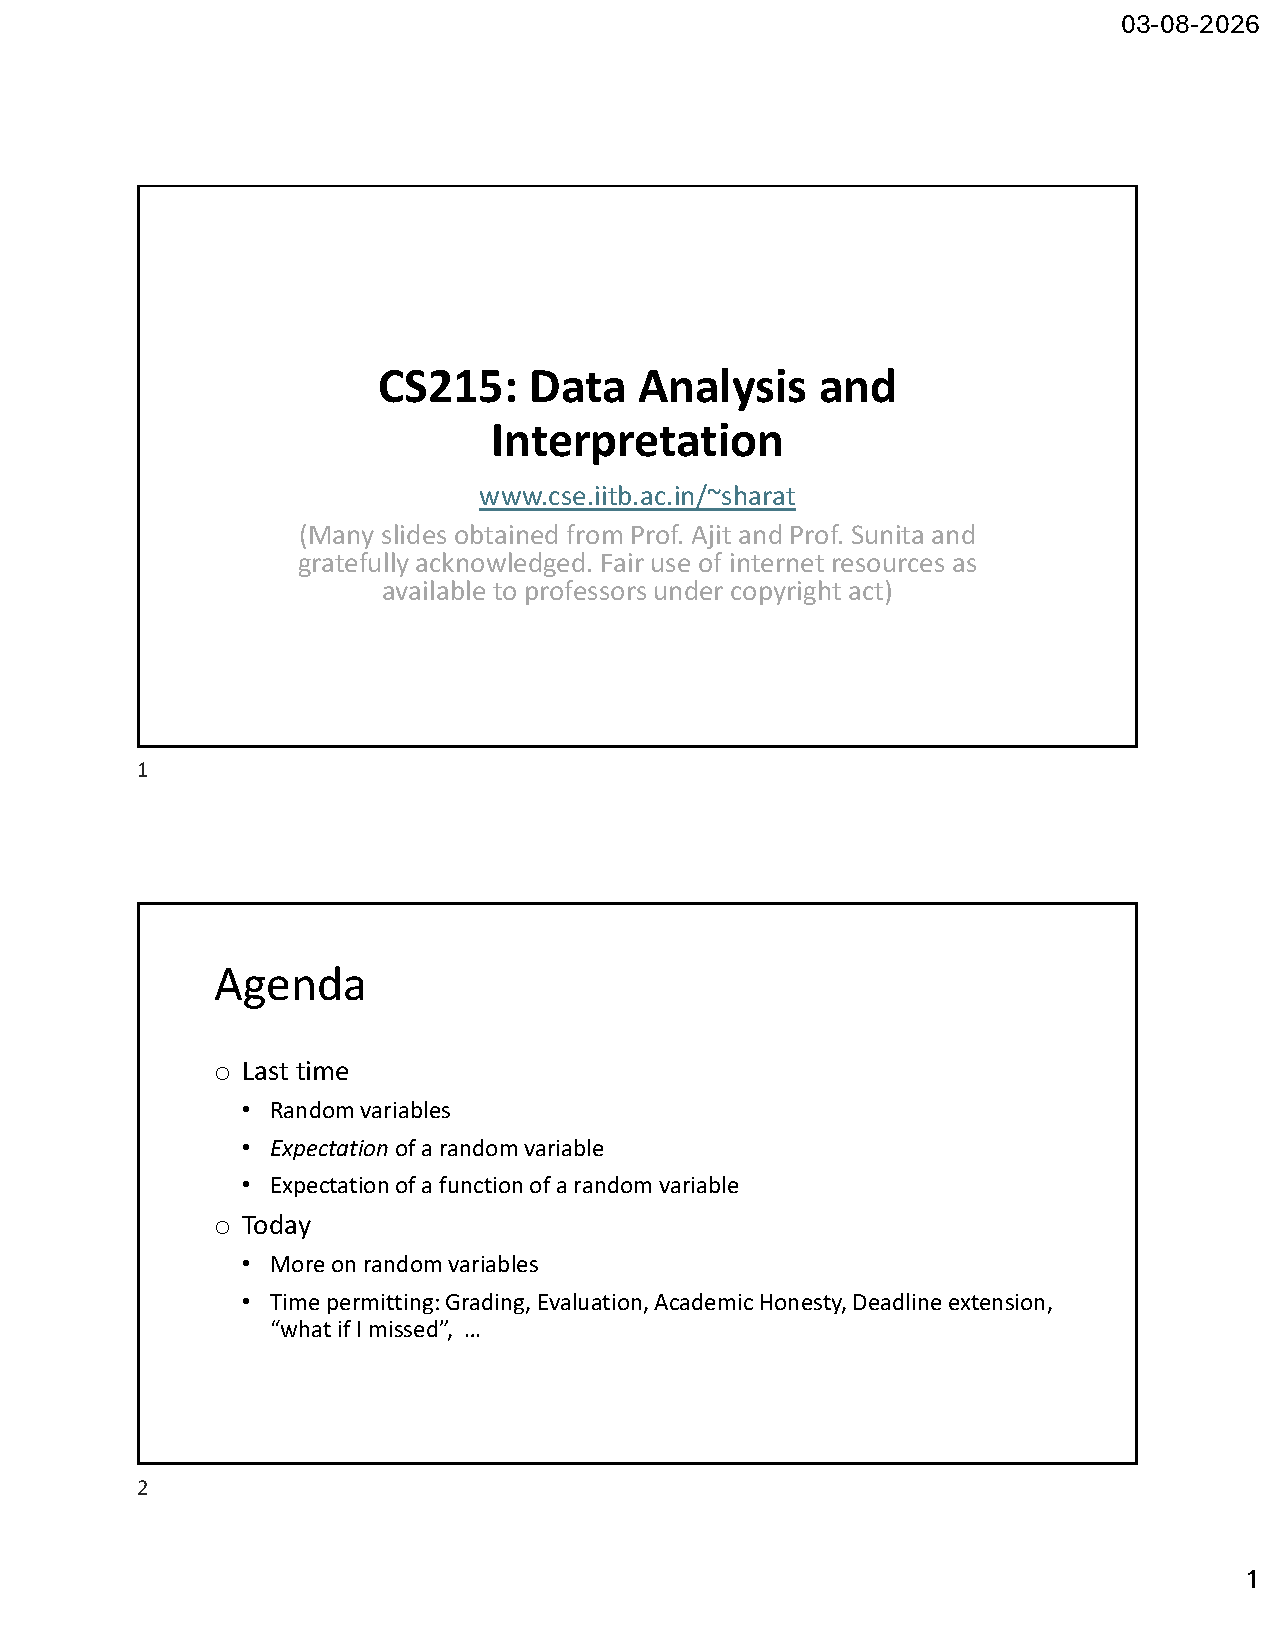
\includepdf[pages=-]{Lec04.pdf}
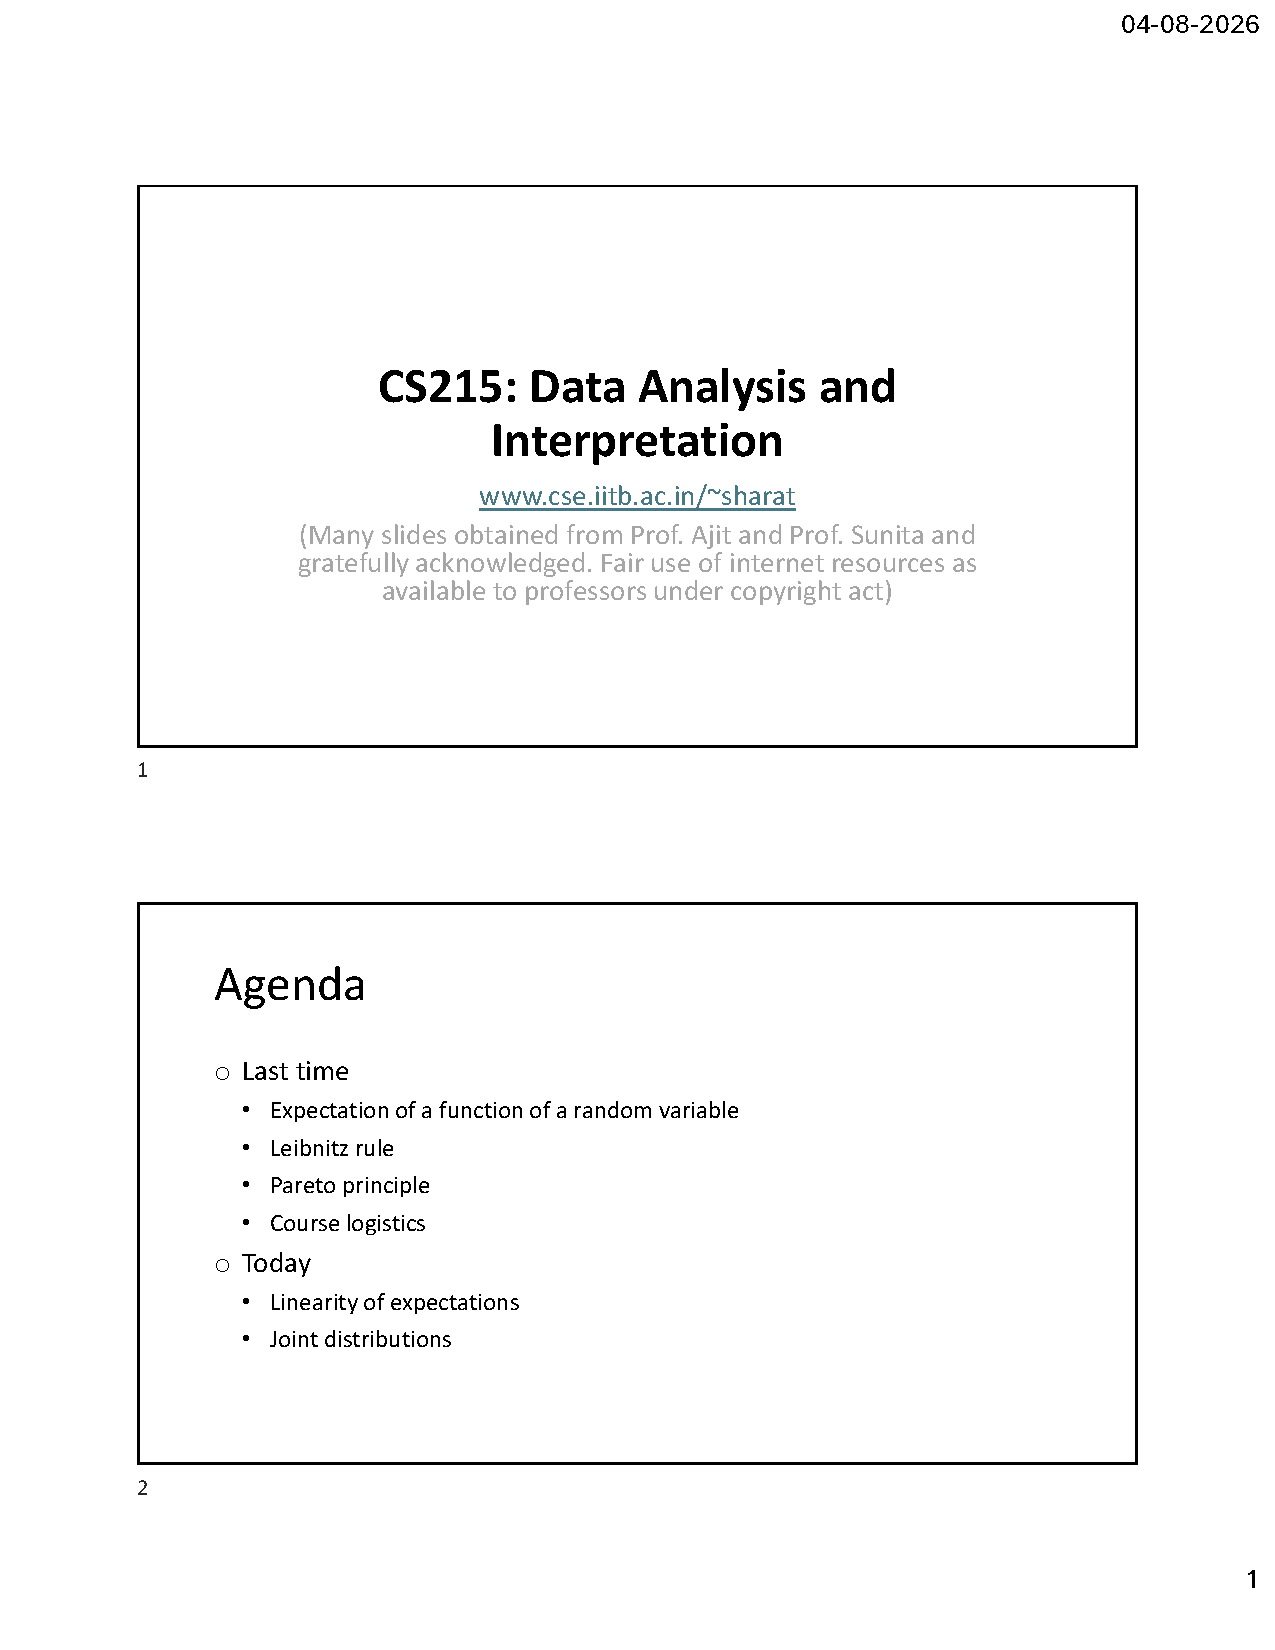
\includepdf[pages={1-6}]{Lec05.pdf}
}


\subsection{Joint Probability, Marginalization, Conditional Probability}
{
\setbeamercolor{background canvas}{bg=} 
\includepdf[pages={7-9}]{Lec05.pdf}
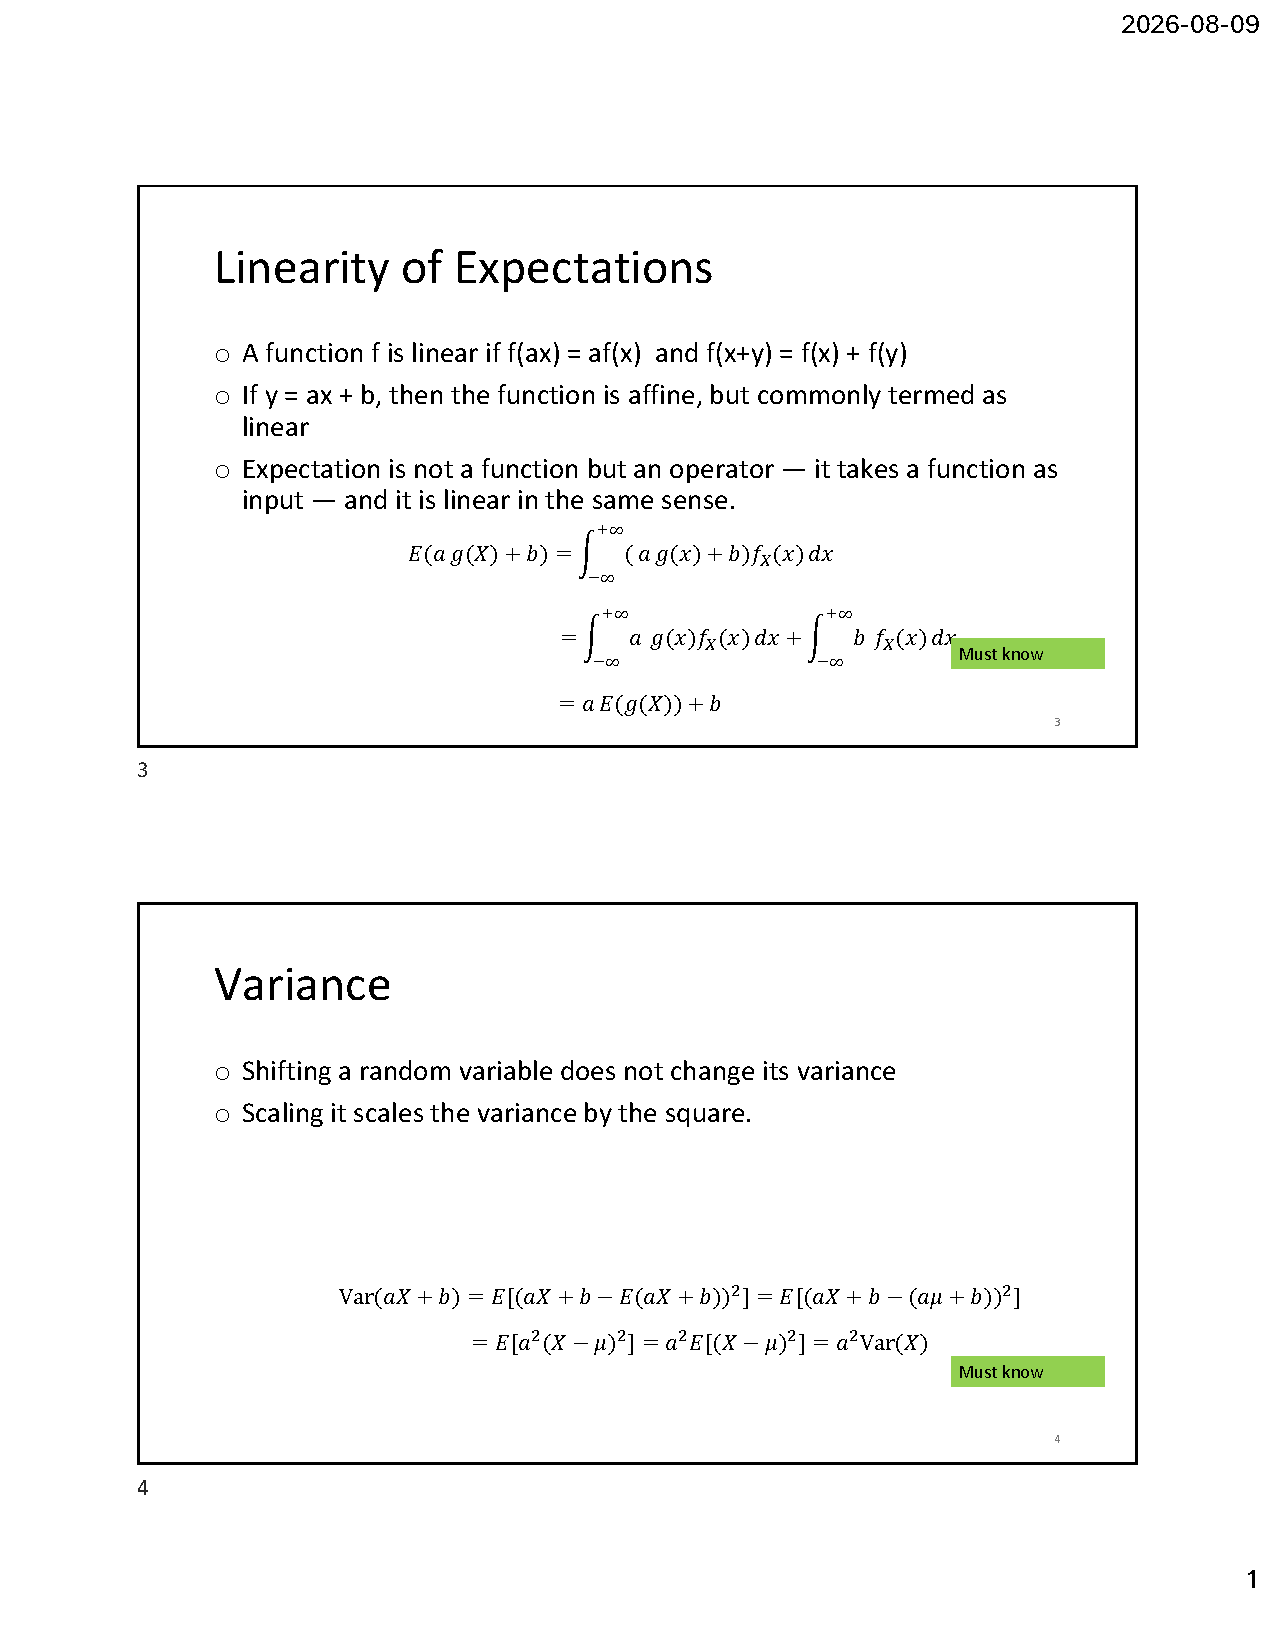
\includepdf[pages=-]{Lec06.pdf}
}

\subsection{Independence, Covariance}
{
\setbeamercolor{background canvas}{bg=} 
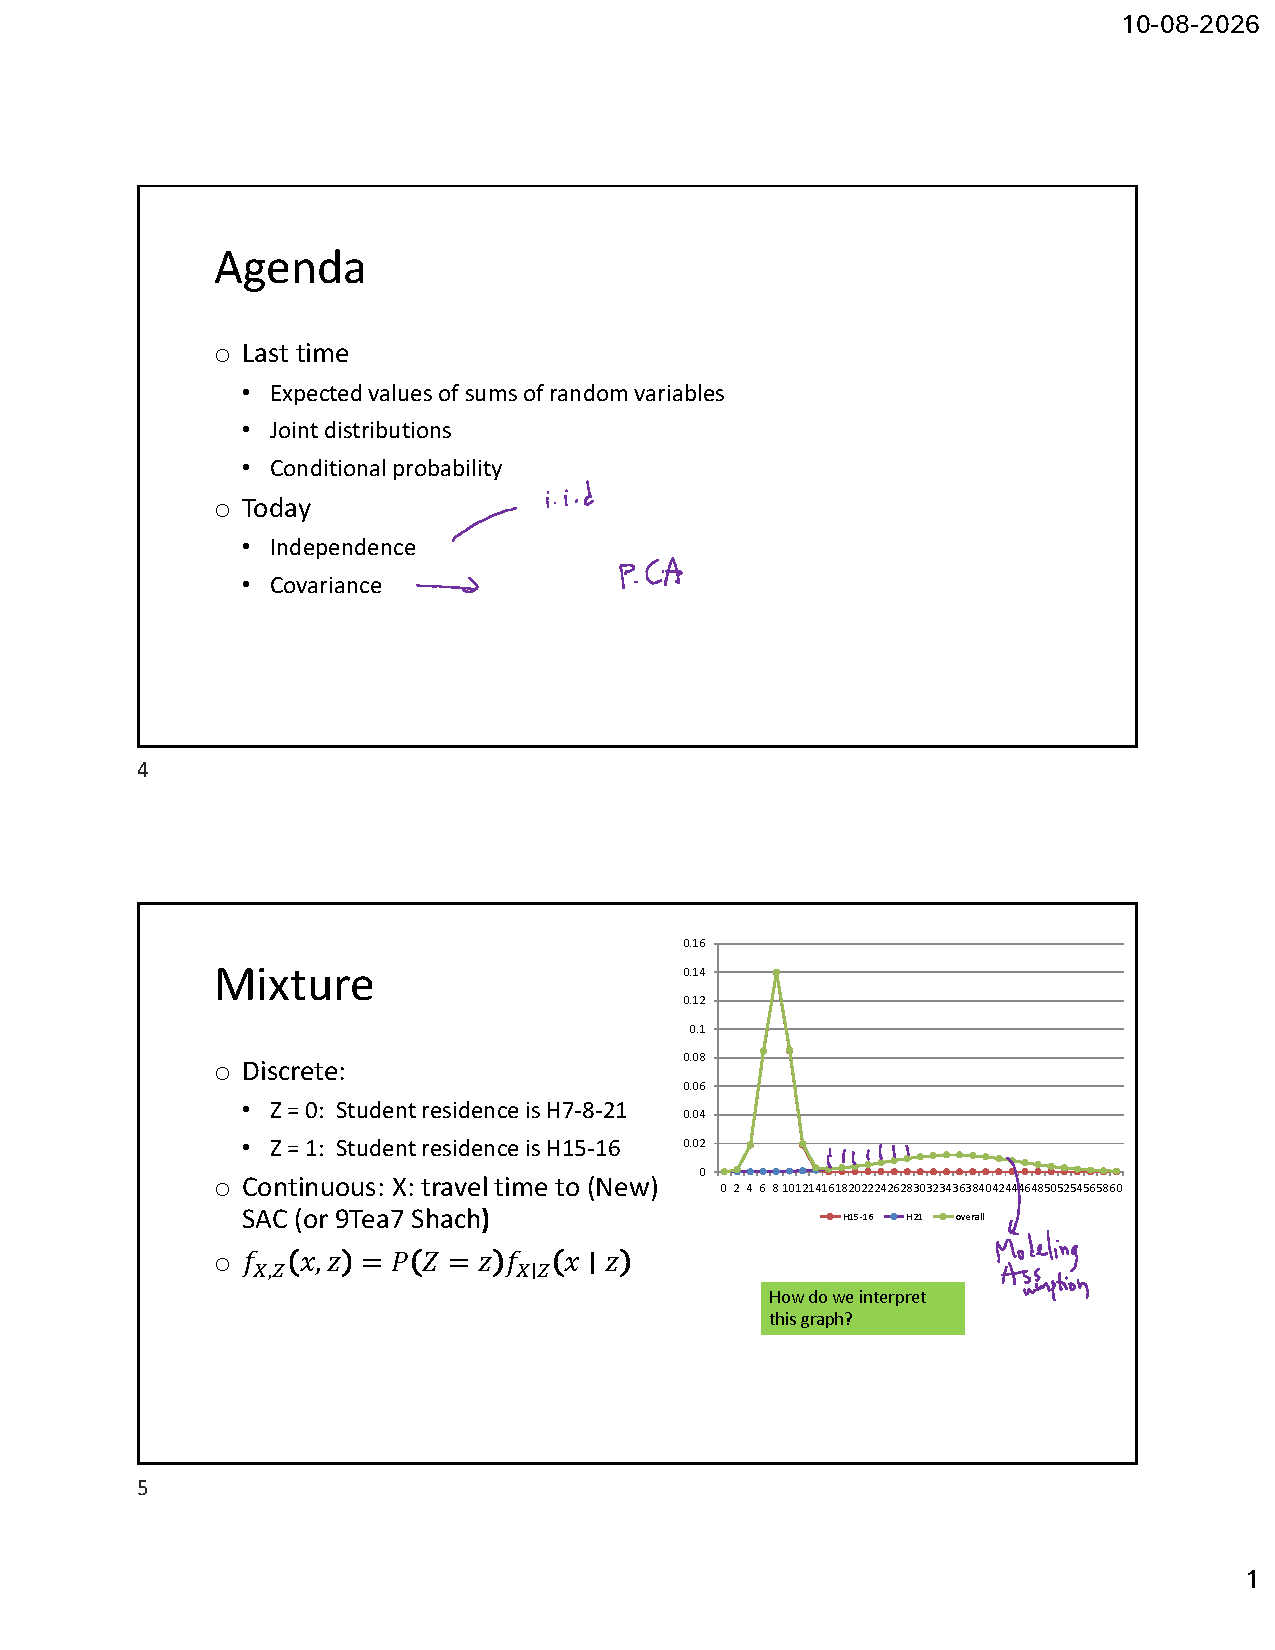
\includepdf[pages=-]{Lec07.pdf}
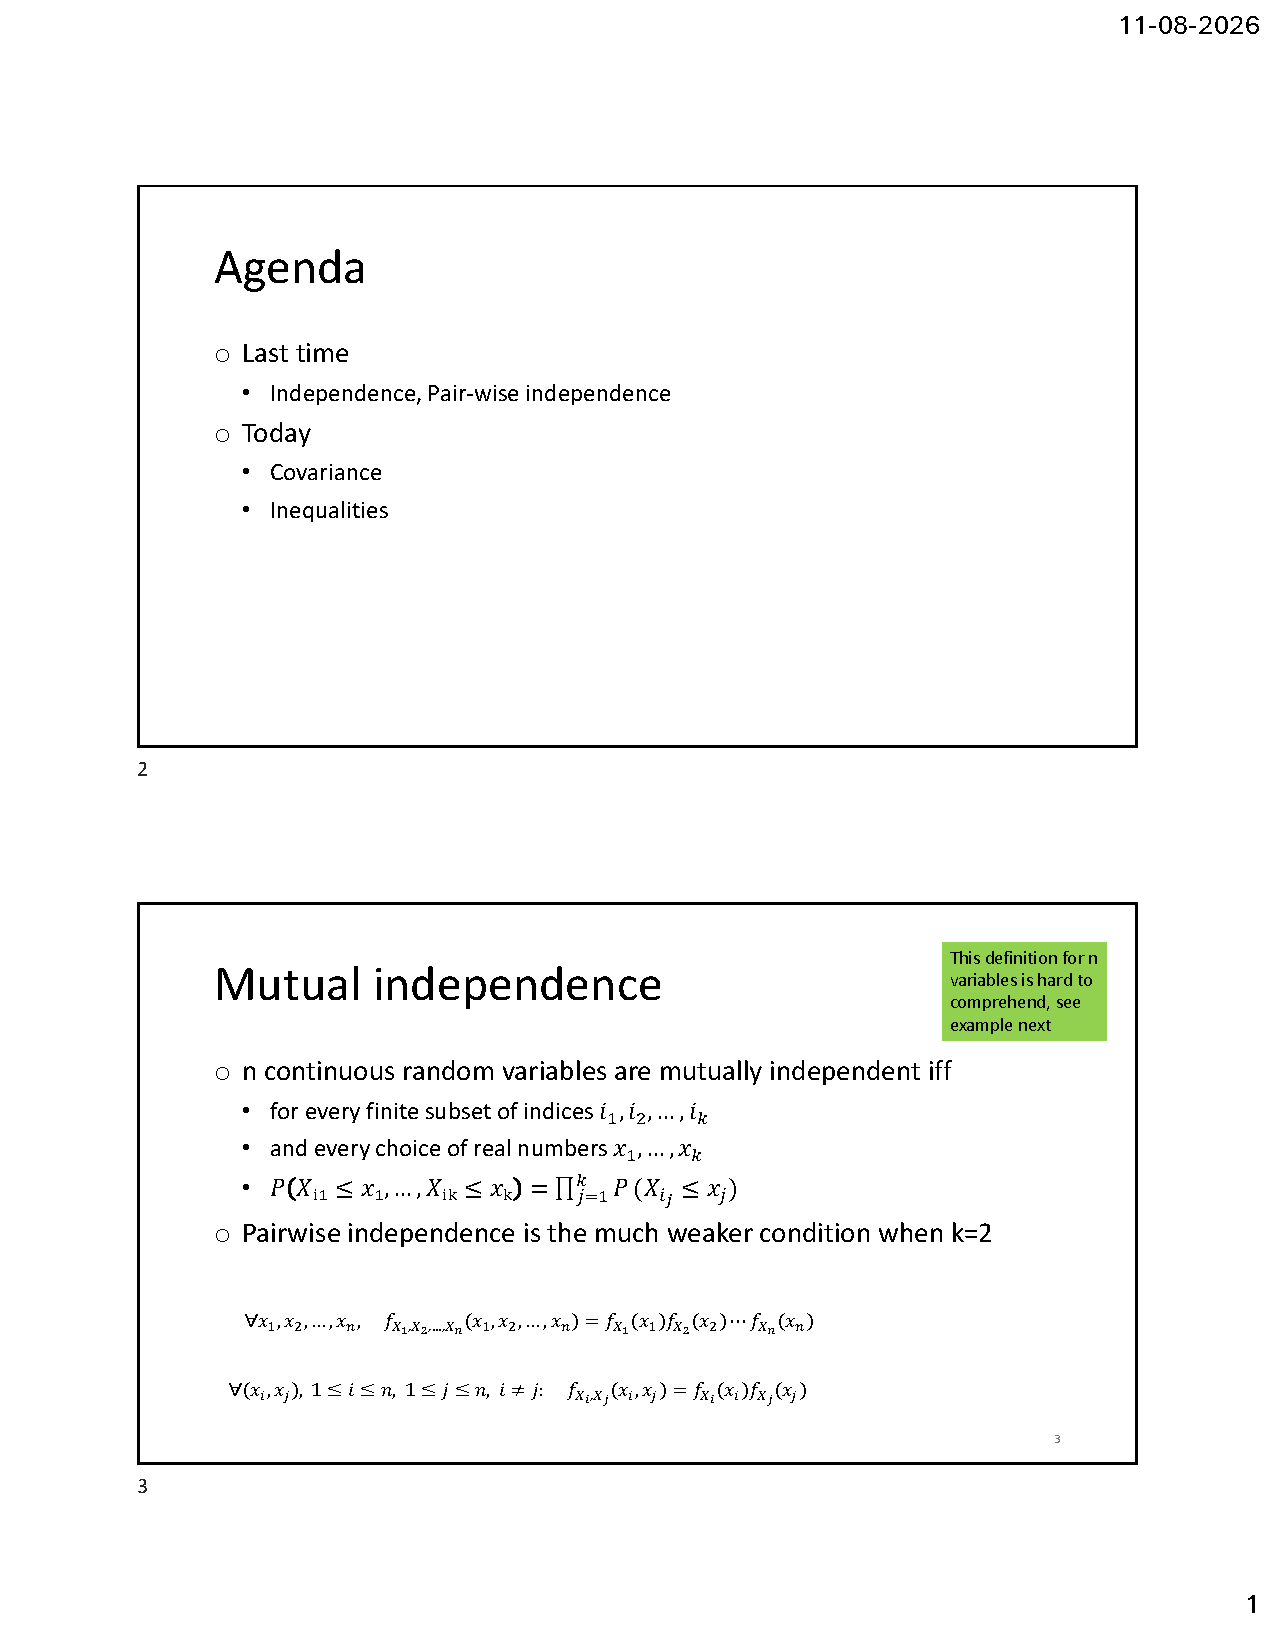
\includepdf[pages=-]{Lec08.pdf}
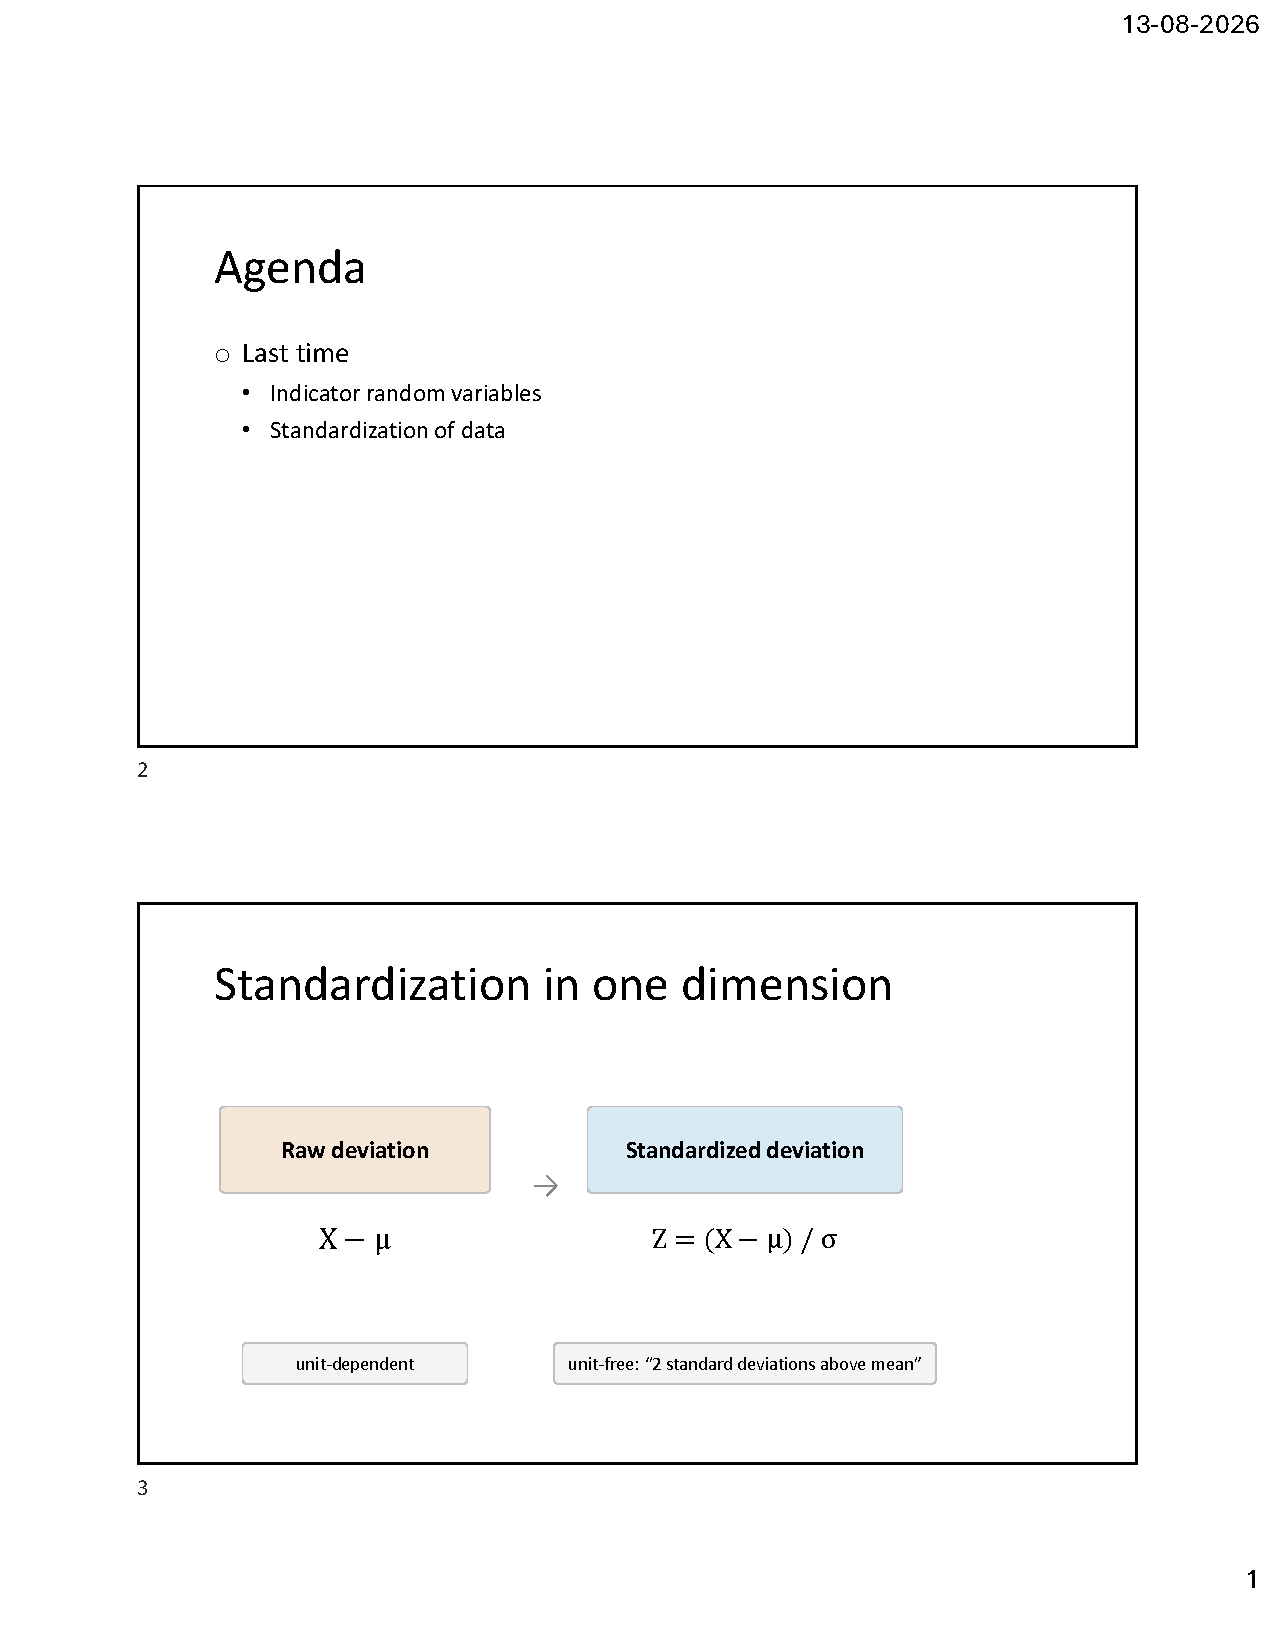
\includepdf[pages={1-3}]{Lec09.pdf}
}


\subsection{Inequalities}
{
\setbeamercolor{background canvas}{bg=} 
\includepdf[pages={4-9}]{Lec09.pdf}
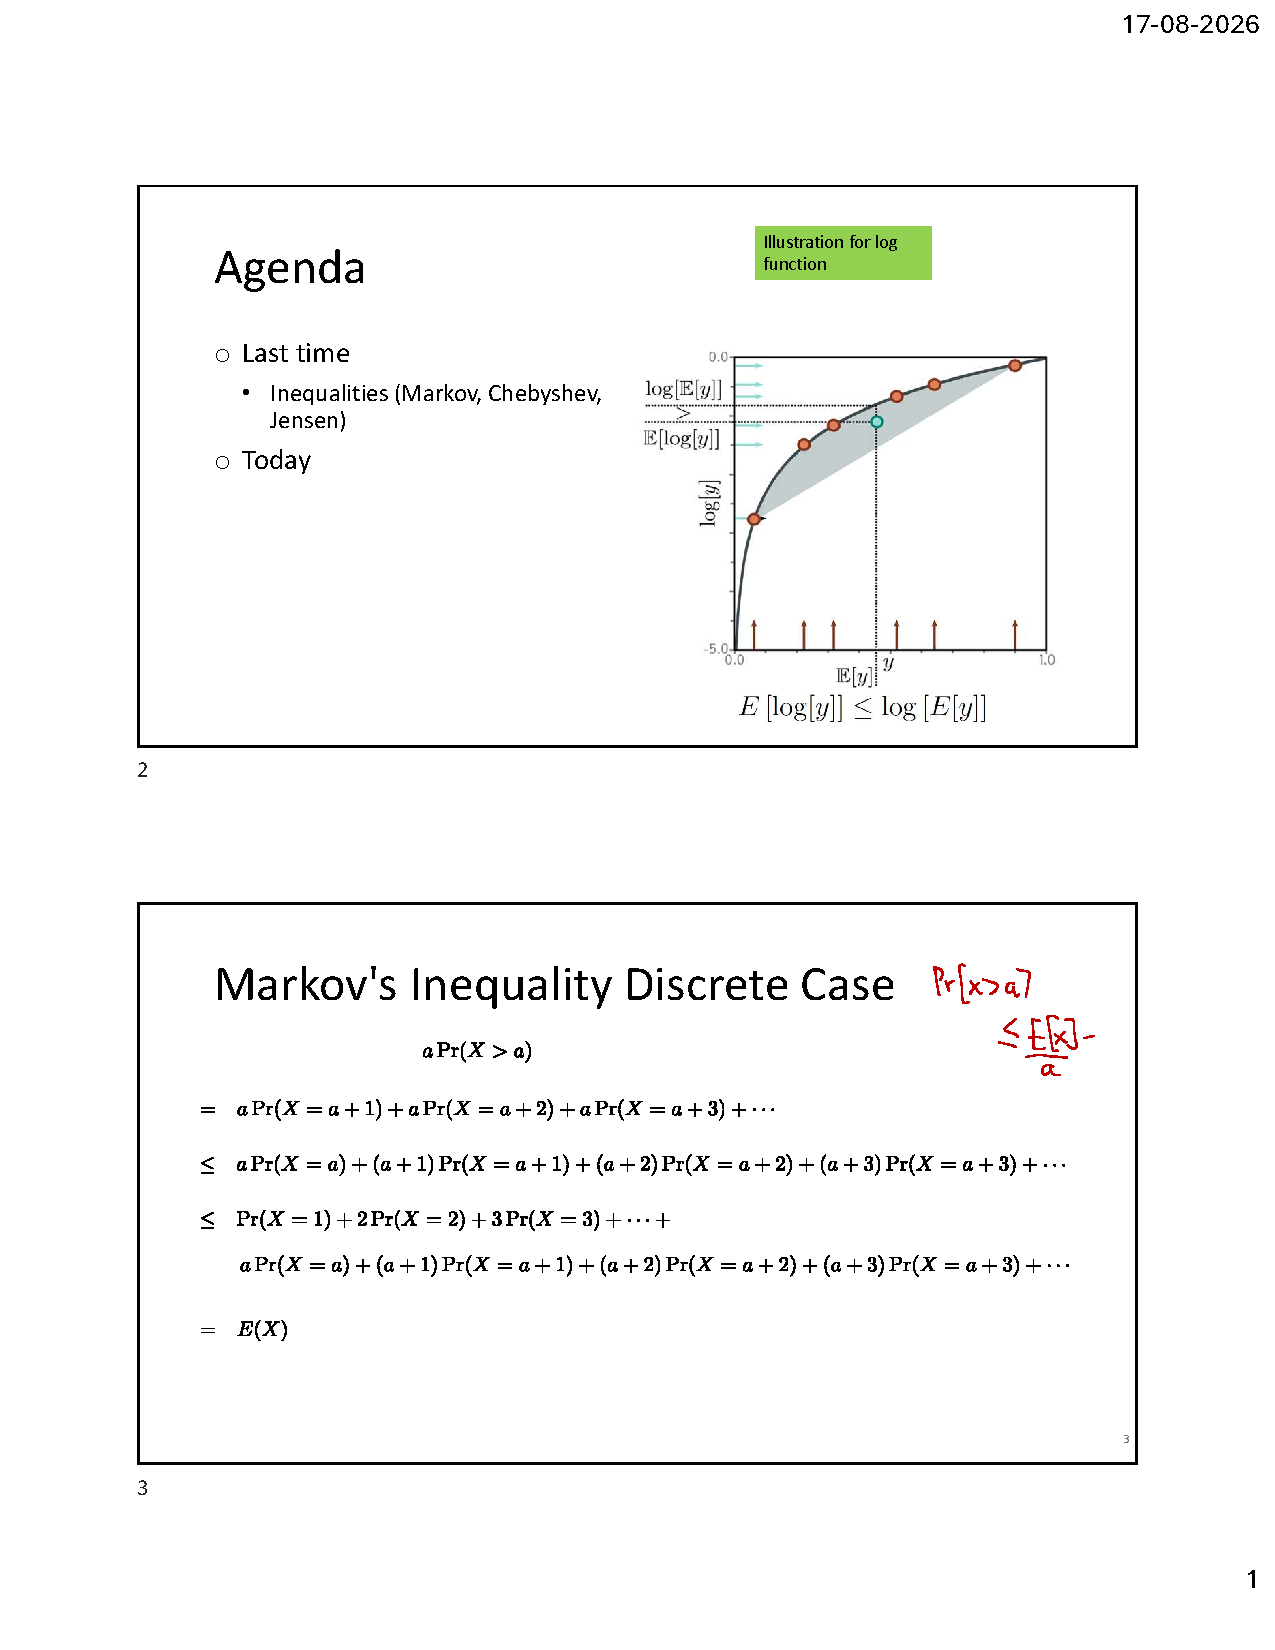
\includepdf[pages=-]{Lec10.pdf}
}

\section{Common Distributions}
\subsection{Binomial distribution, Urn Model}
{
\setbeamercolor{background canvas}{bg=} 
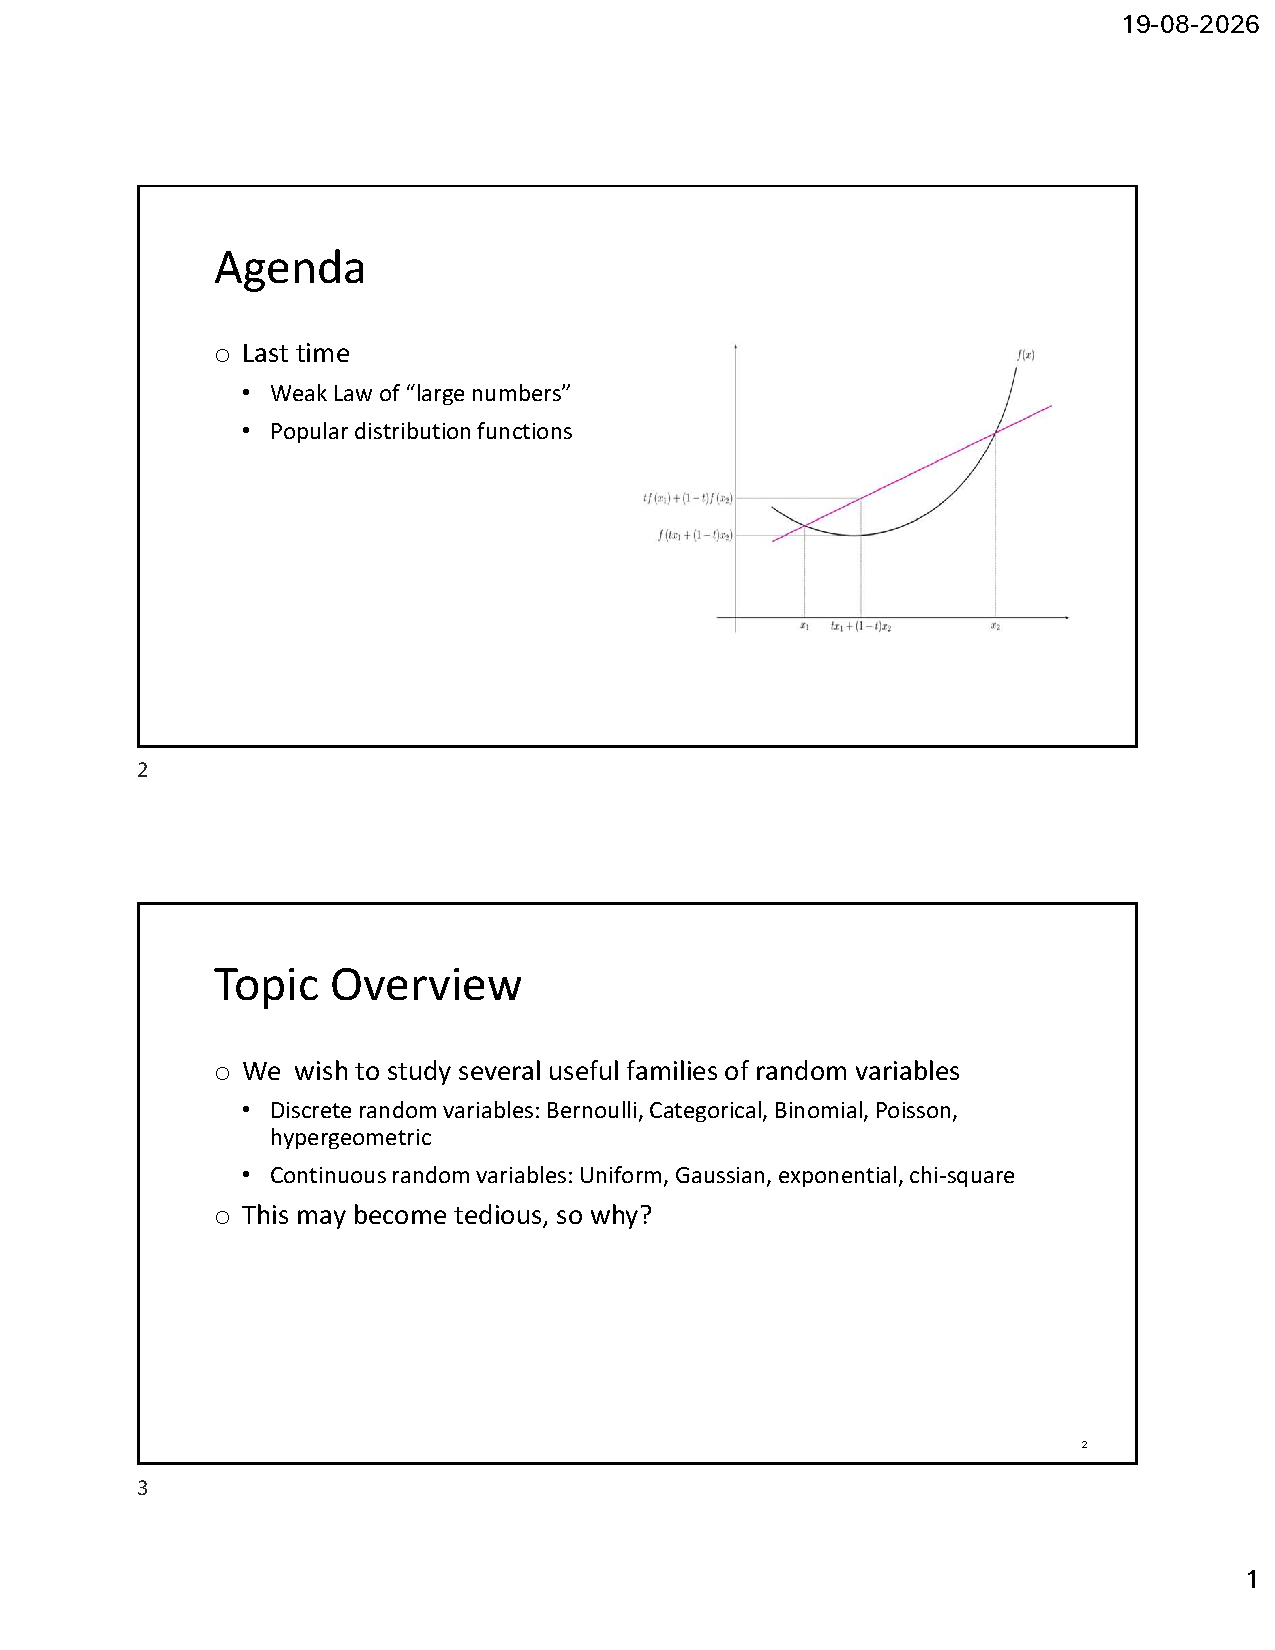
\includepdf[pages=-]{Lec11.pdf}
}

\subsection{Geometric Distribution, Mean and Variance using MGF}
{
\setbeamercolor{background canvas}{bg=} 
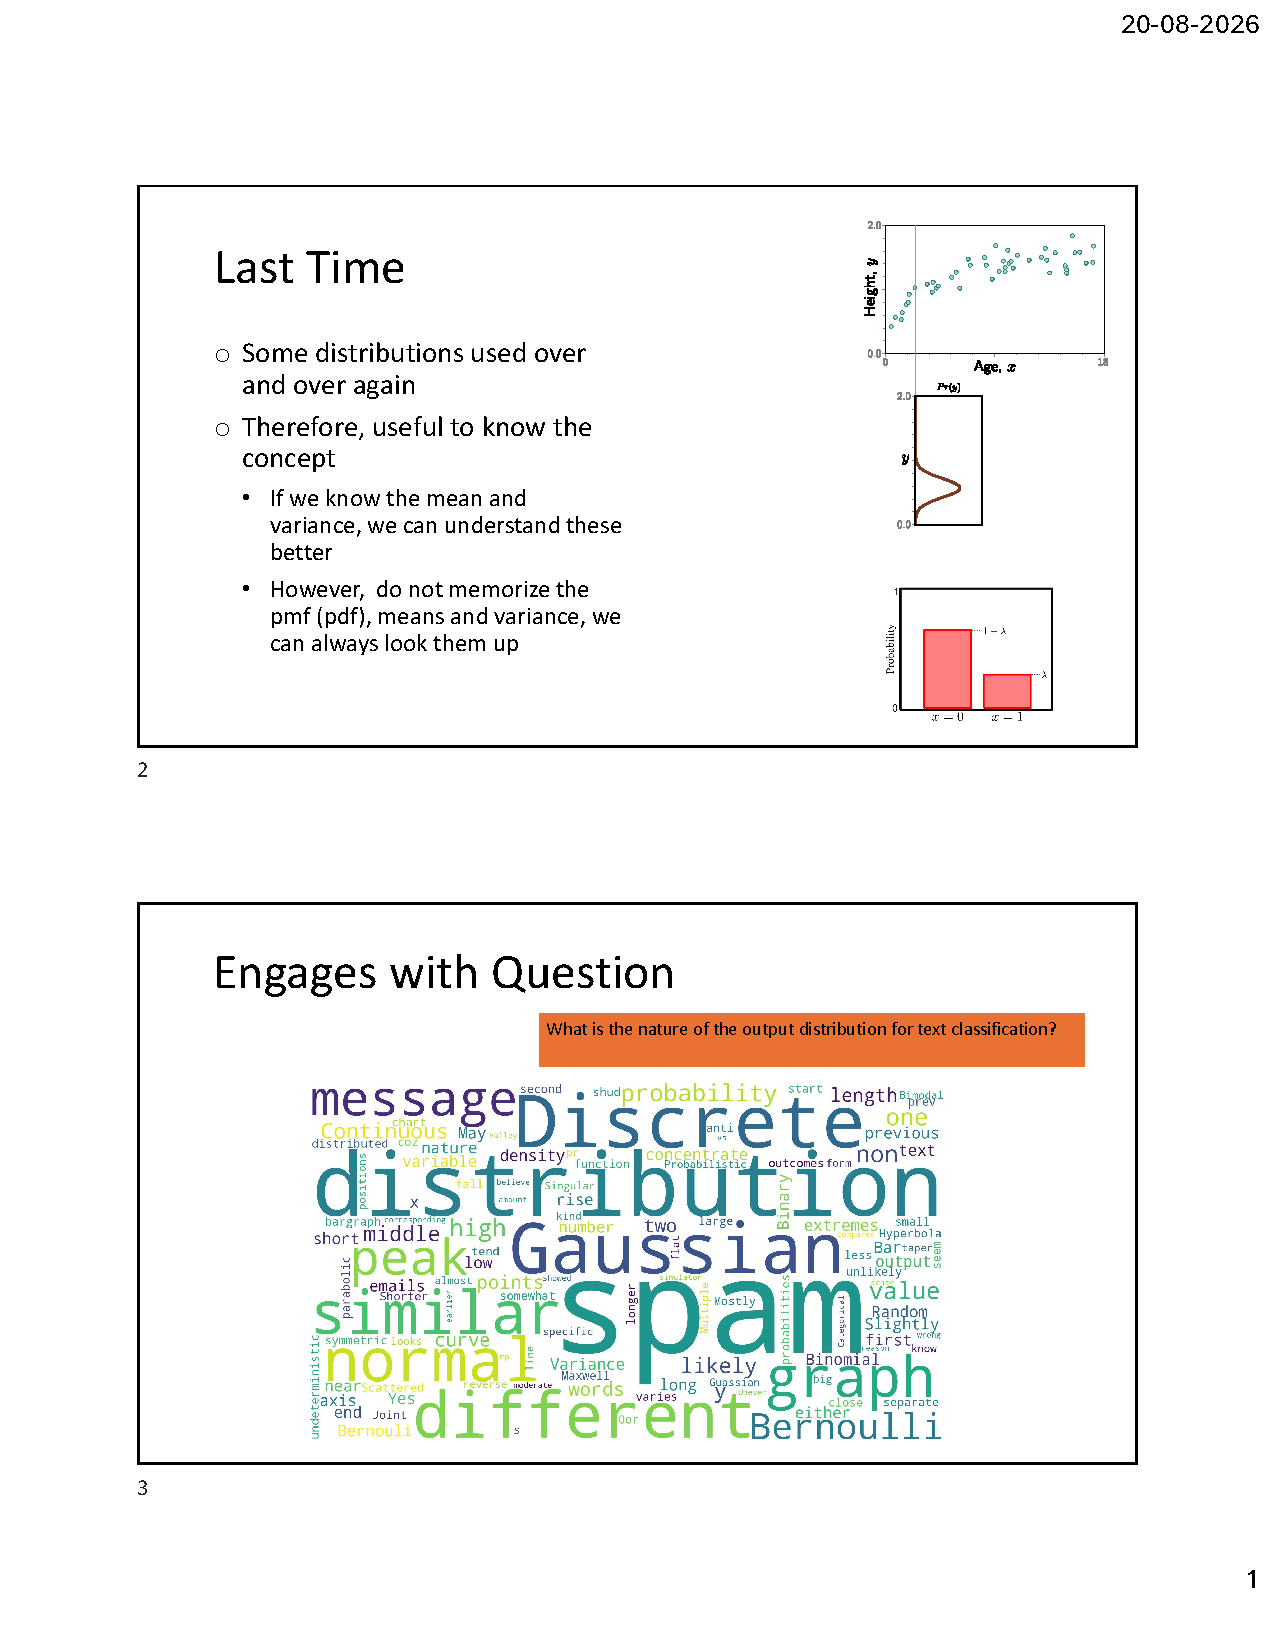
\includepdf[pages=-]{Lec12.pdf}
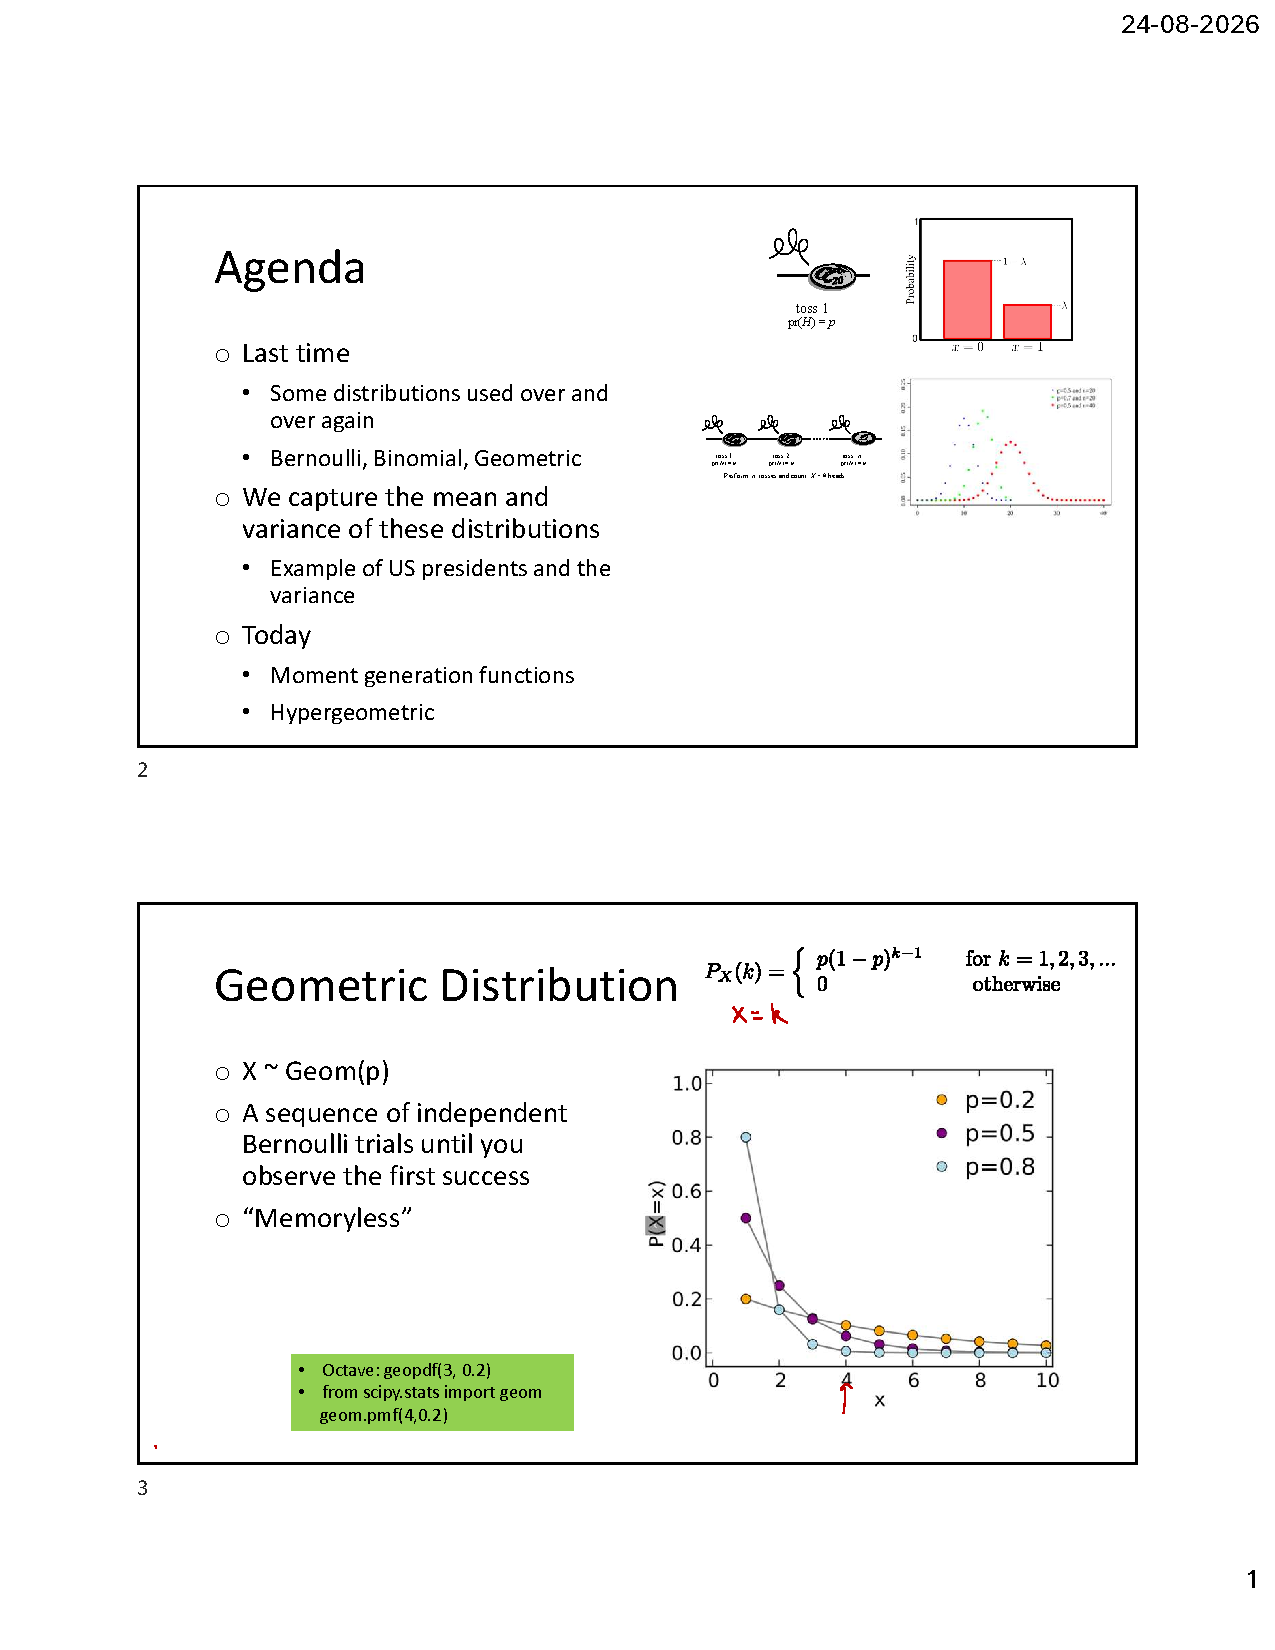
\includepdf[pages=-]{Lec13.pdf}
}

\subsection{Hypergeometric, Continuous Distribution}
{
\setbeamercolor{background canvas}{bg=} 
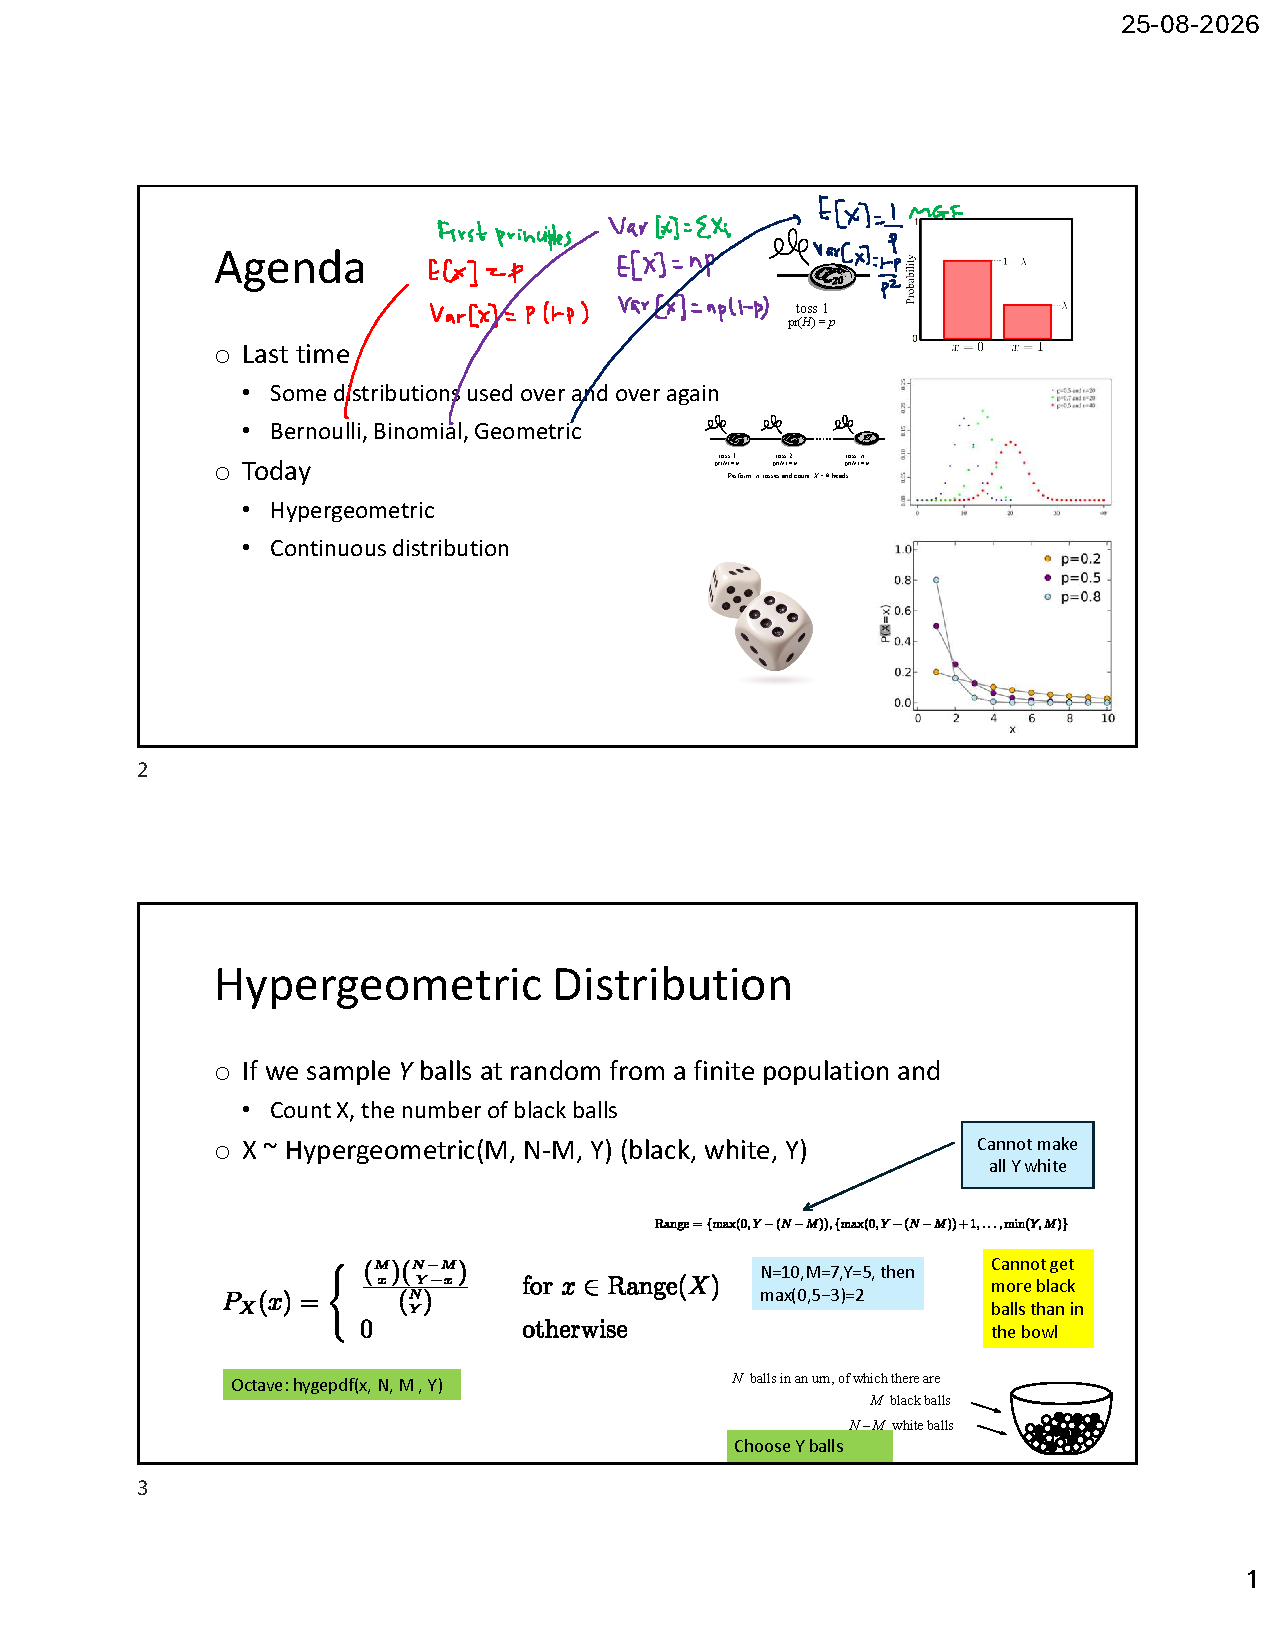
\includepdf[pages=-]{Lec14.pdf}
}

\subsection{PRNG, Random subset}
{
\setbeamercolor{background canvas}{bg=} 
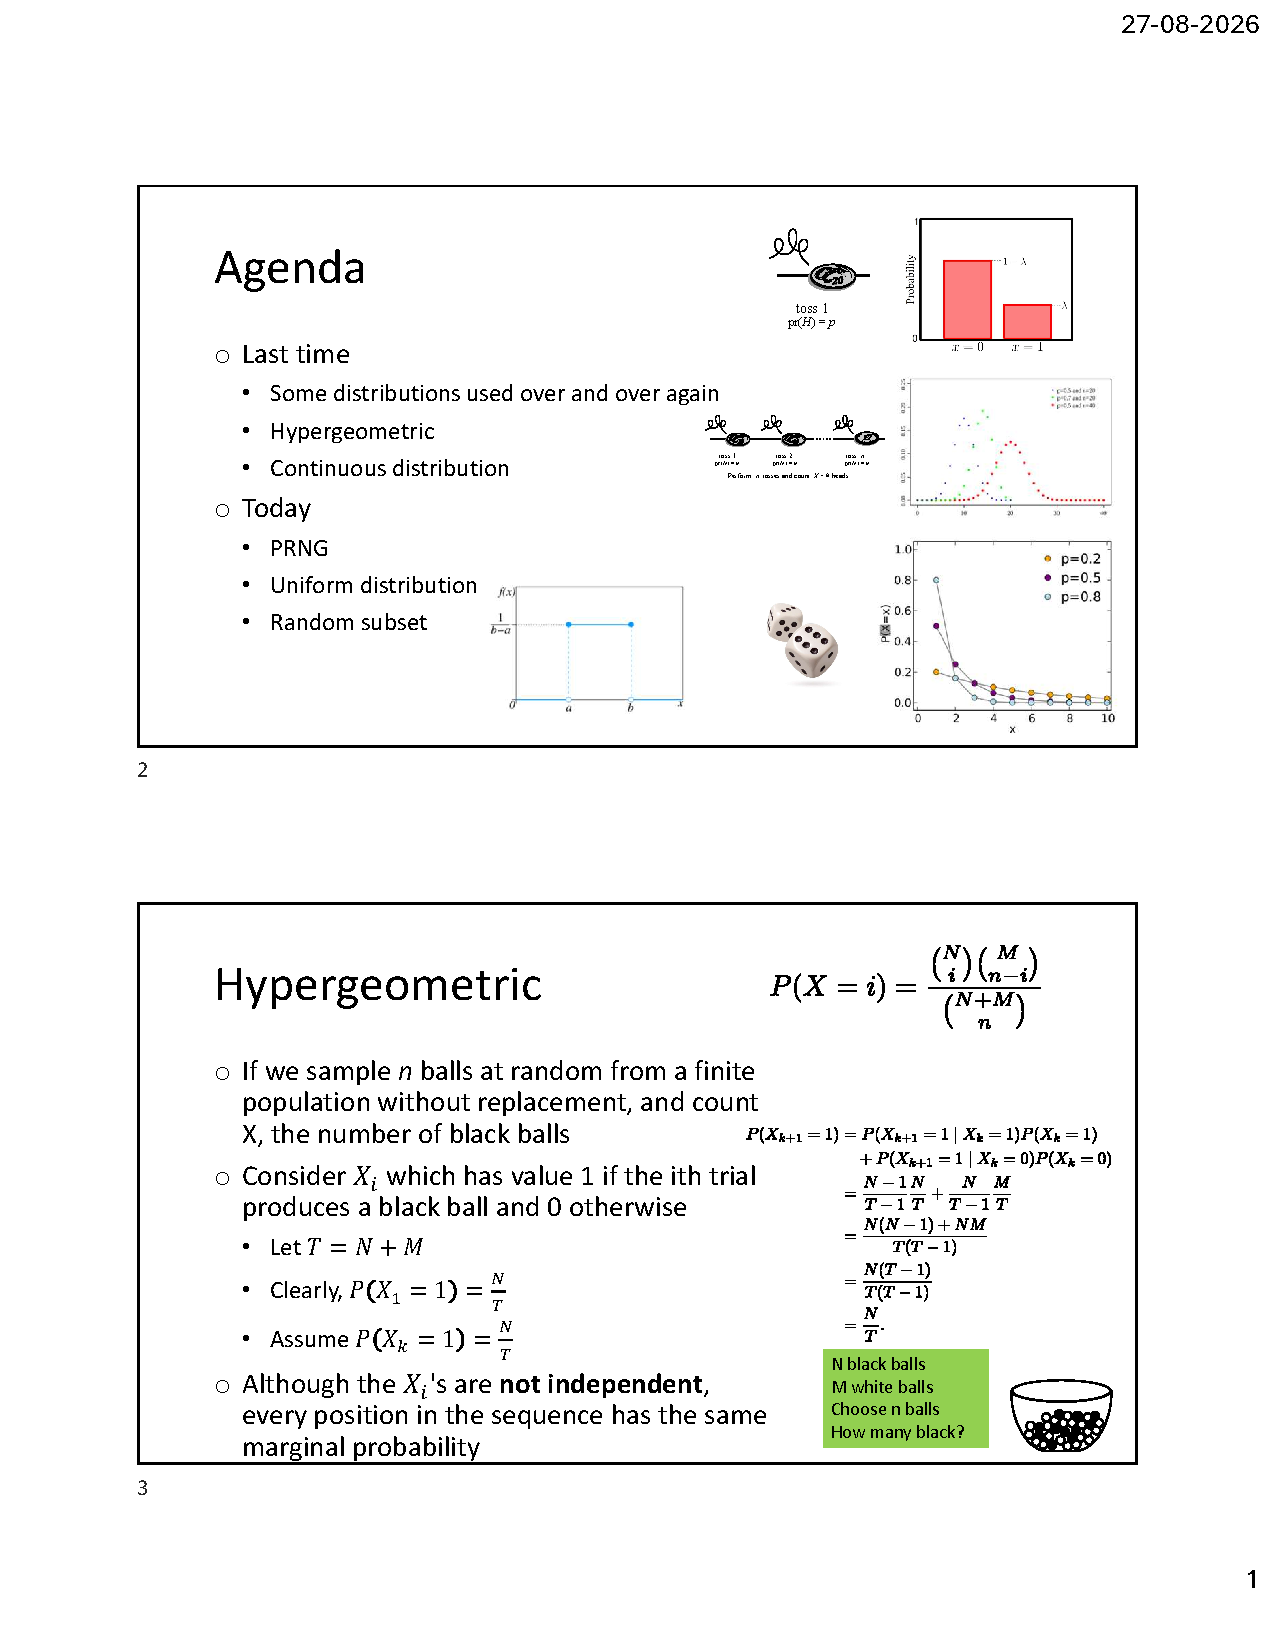
\includepdf[pages=-]{Lec15.pdf}
}

\subsection{Normal Distribution, p-Quantiles and z-Score}
{
\setbeamercolor{background canvas}{bg=} 
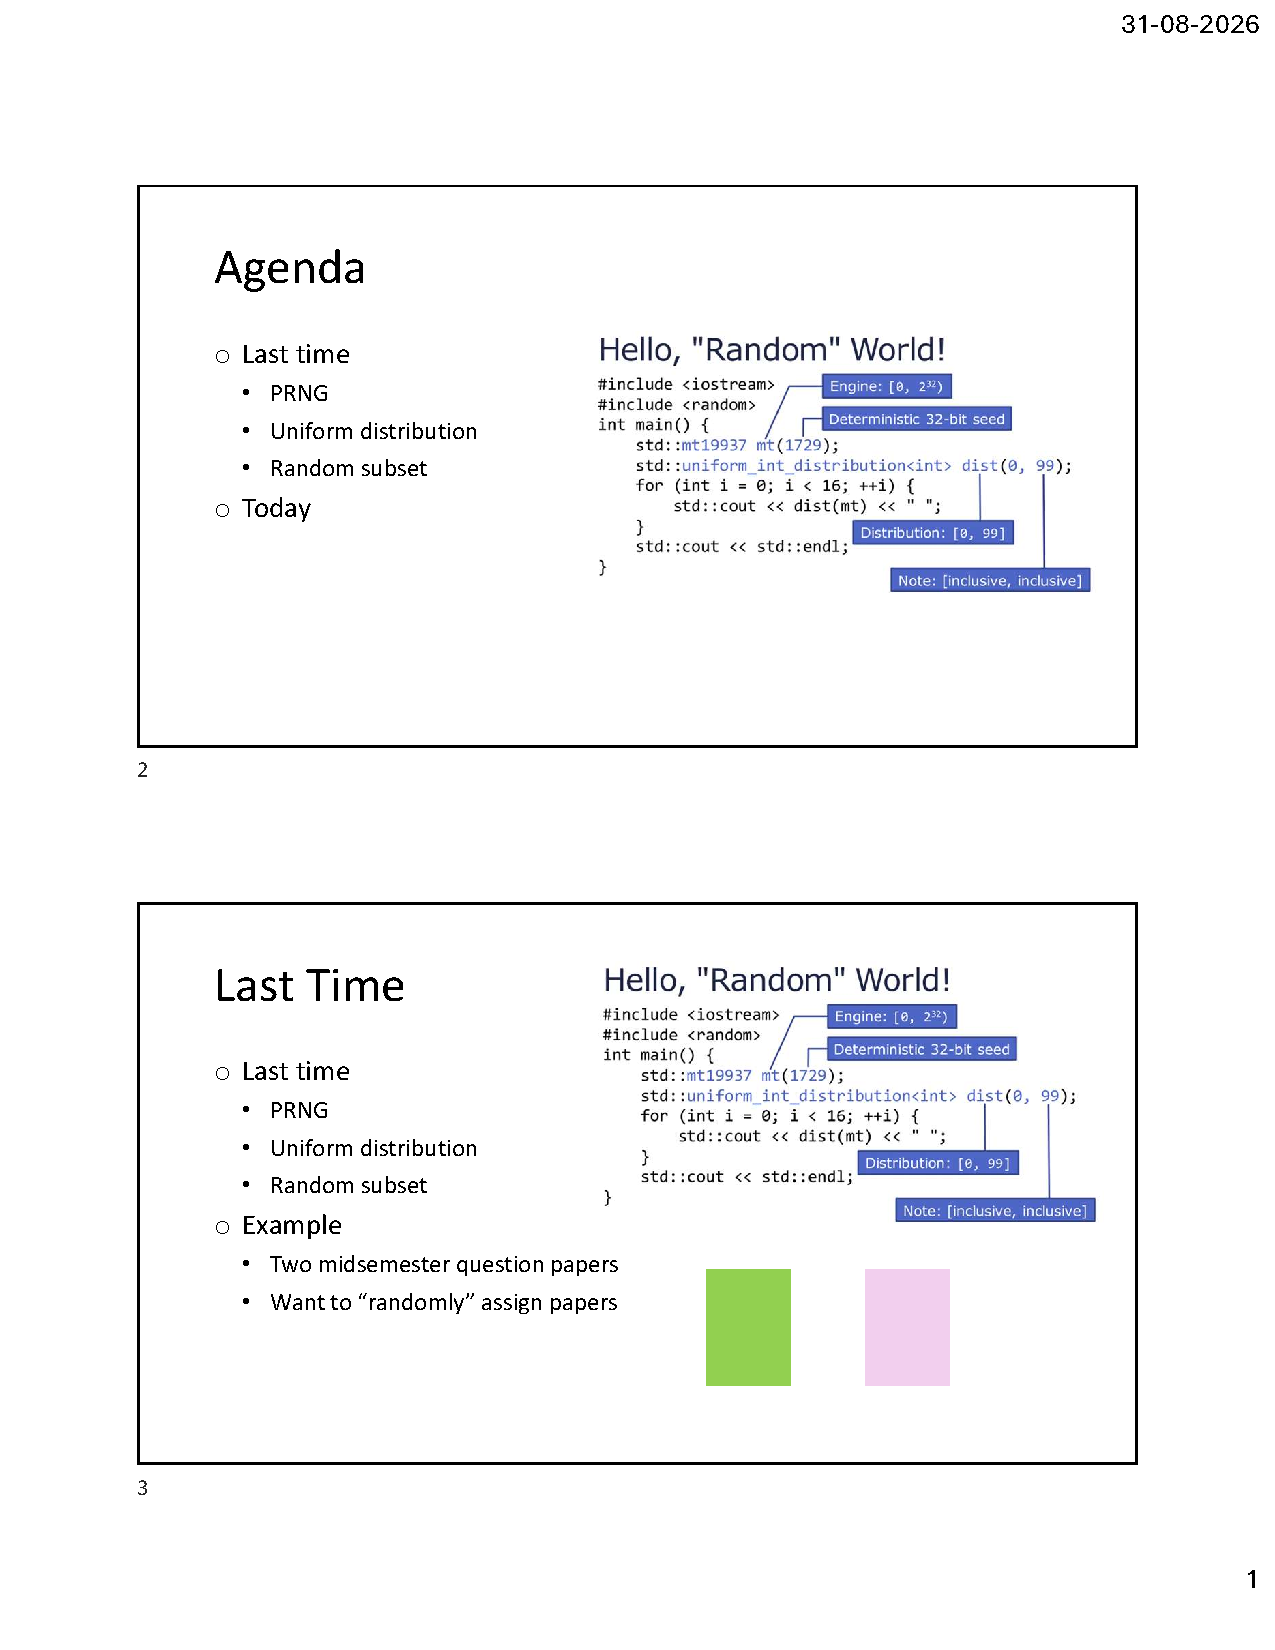
\includepdf[pages=-]{Lec16.pdf}
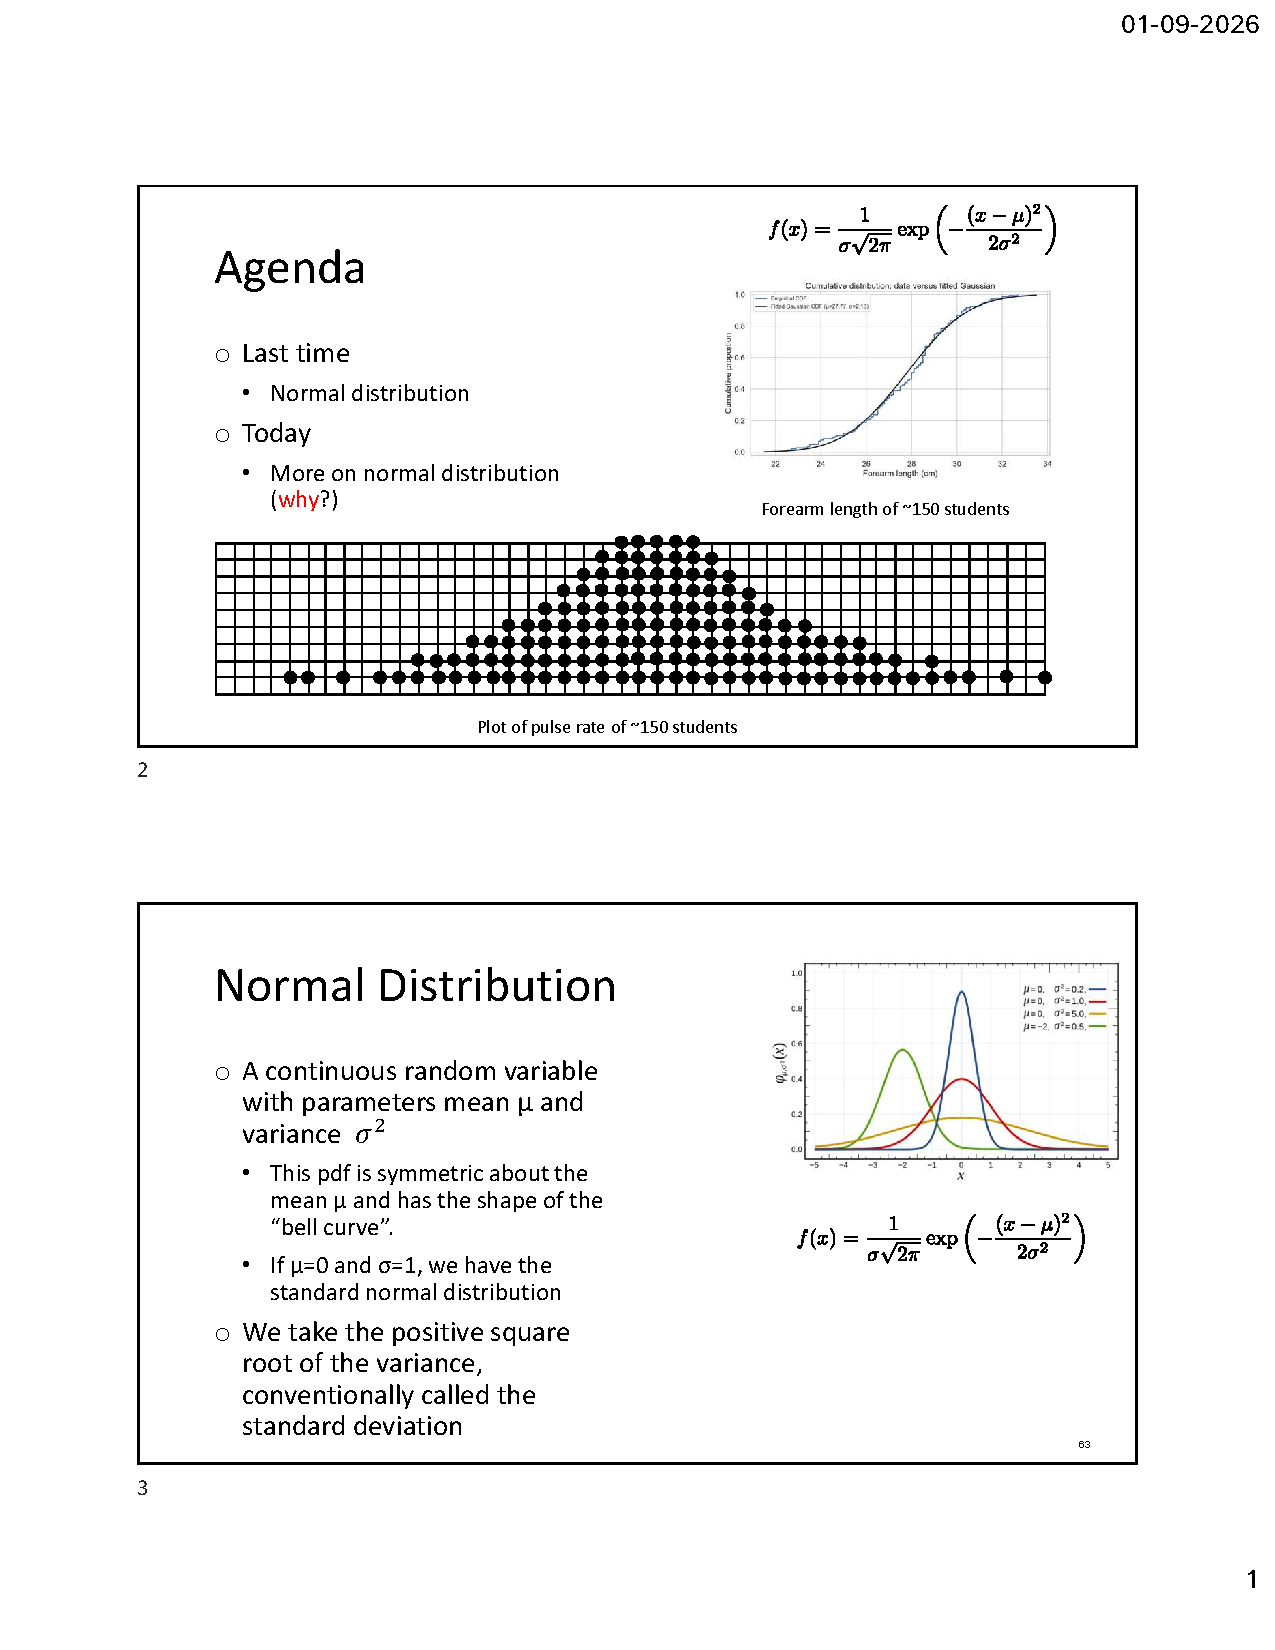
\includepdf[pages=-]{Lec17.pdf}
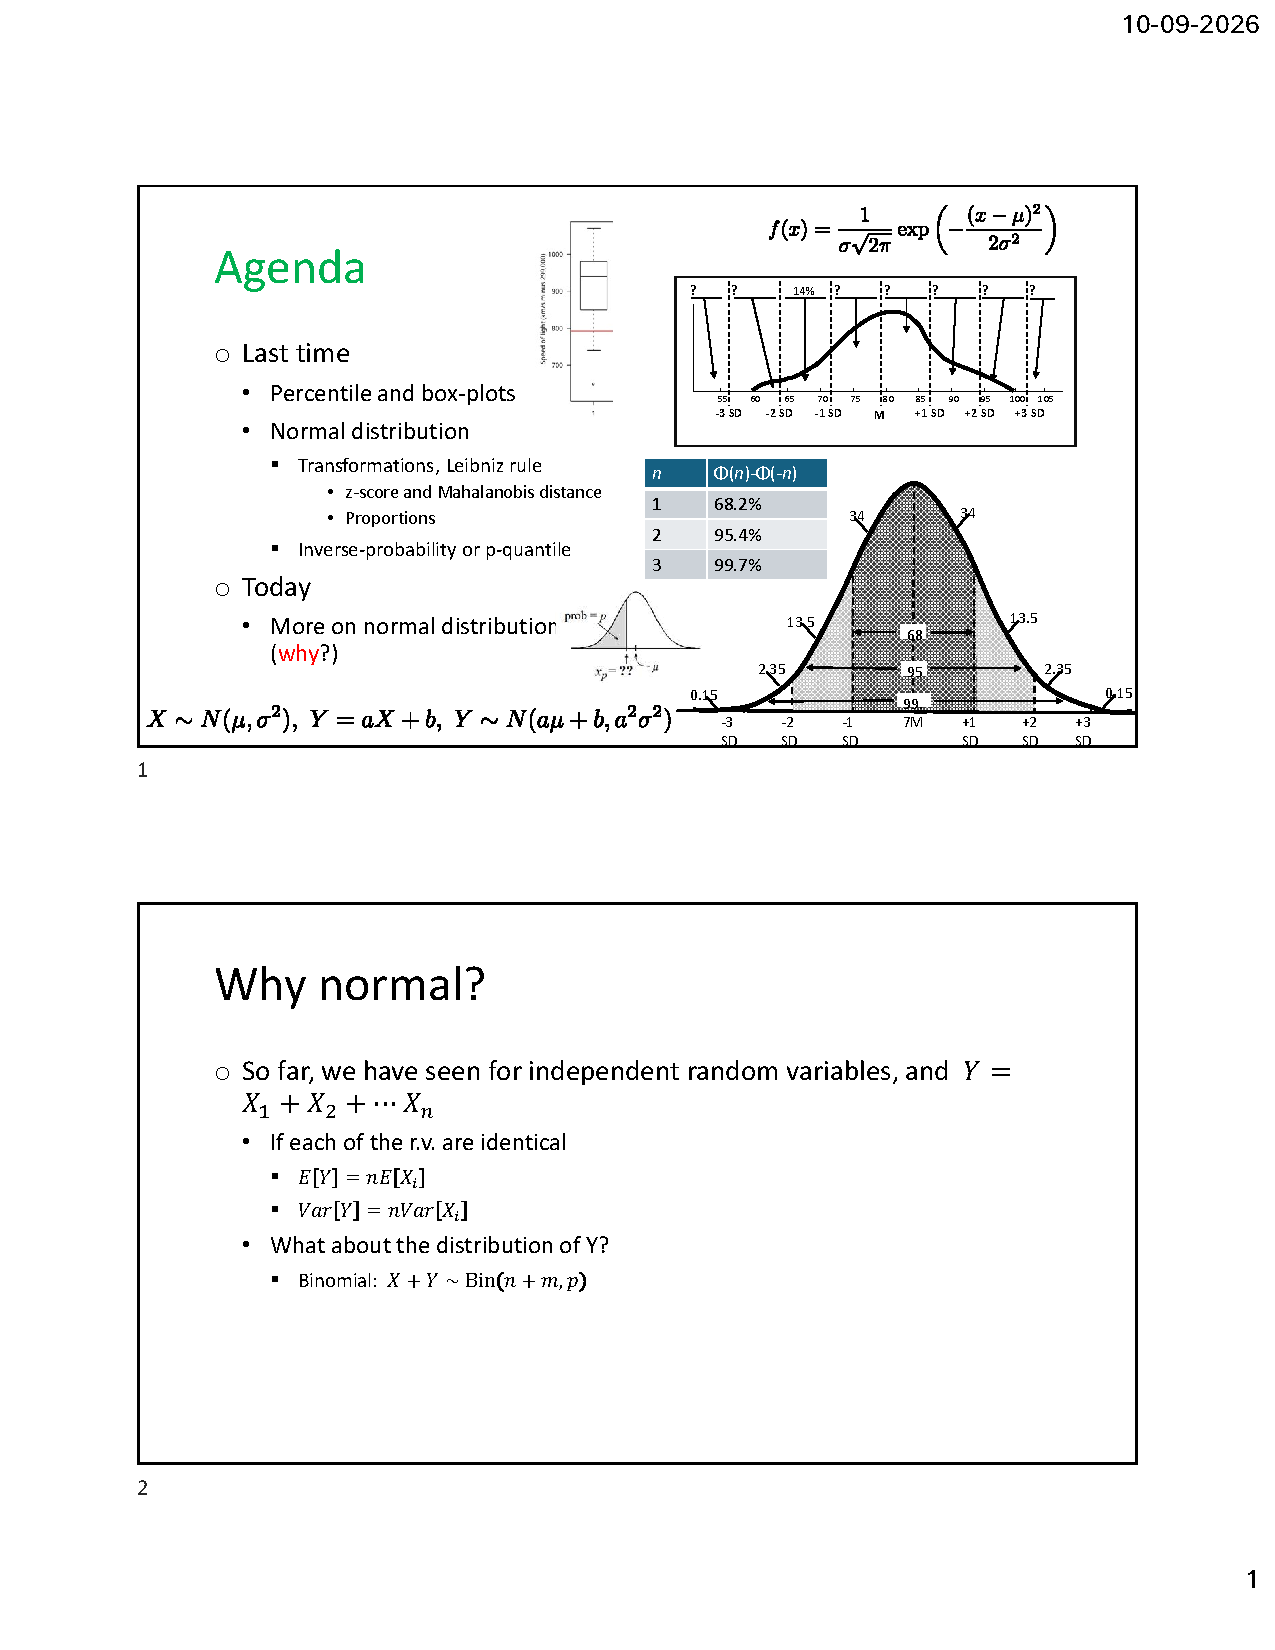
\includepdf[pages=-]{Lec18.pdf}
}


\section{CLT and Sample mean estimators}
\subsection{CLT}
{
\setbeamercolor{background canvas}{bg=} 
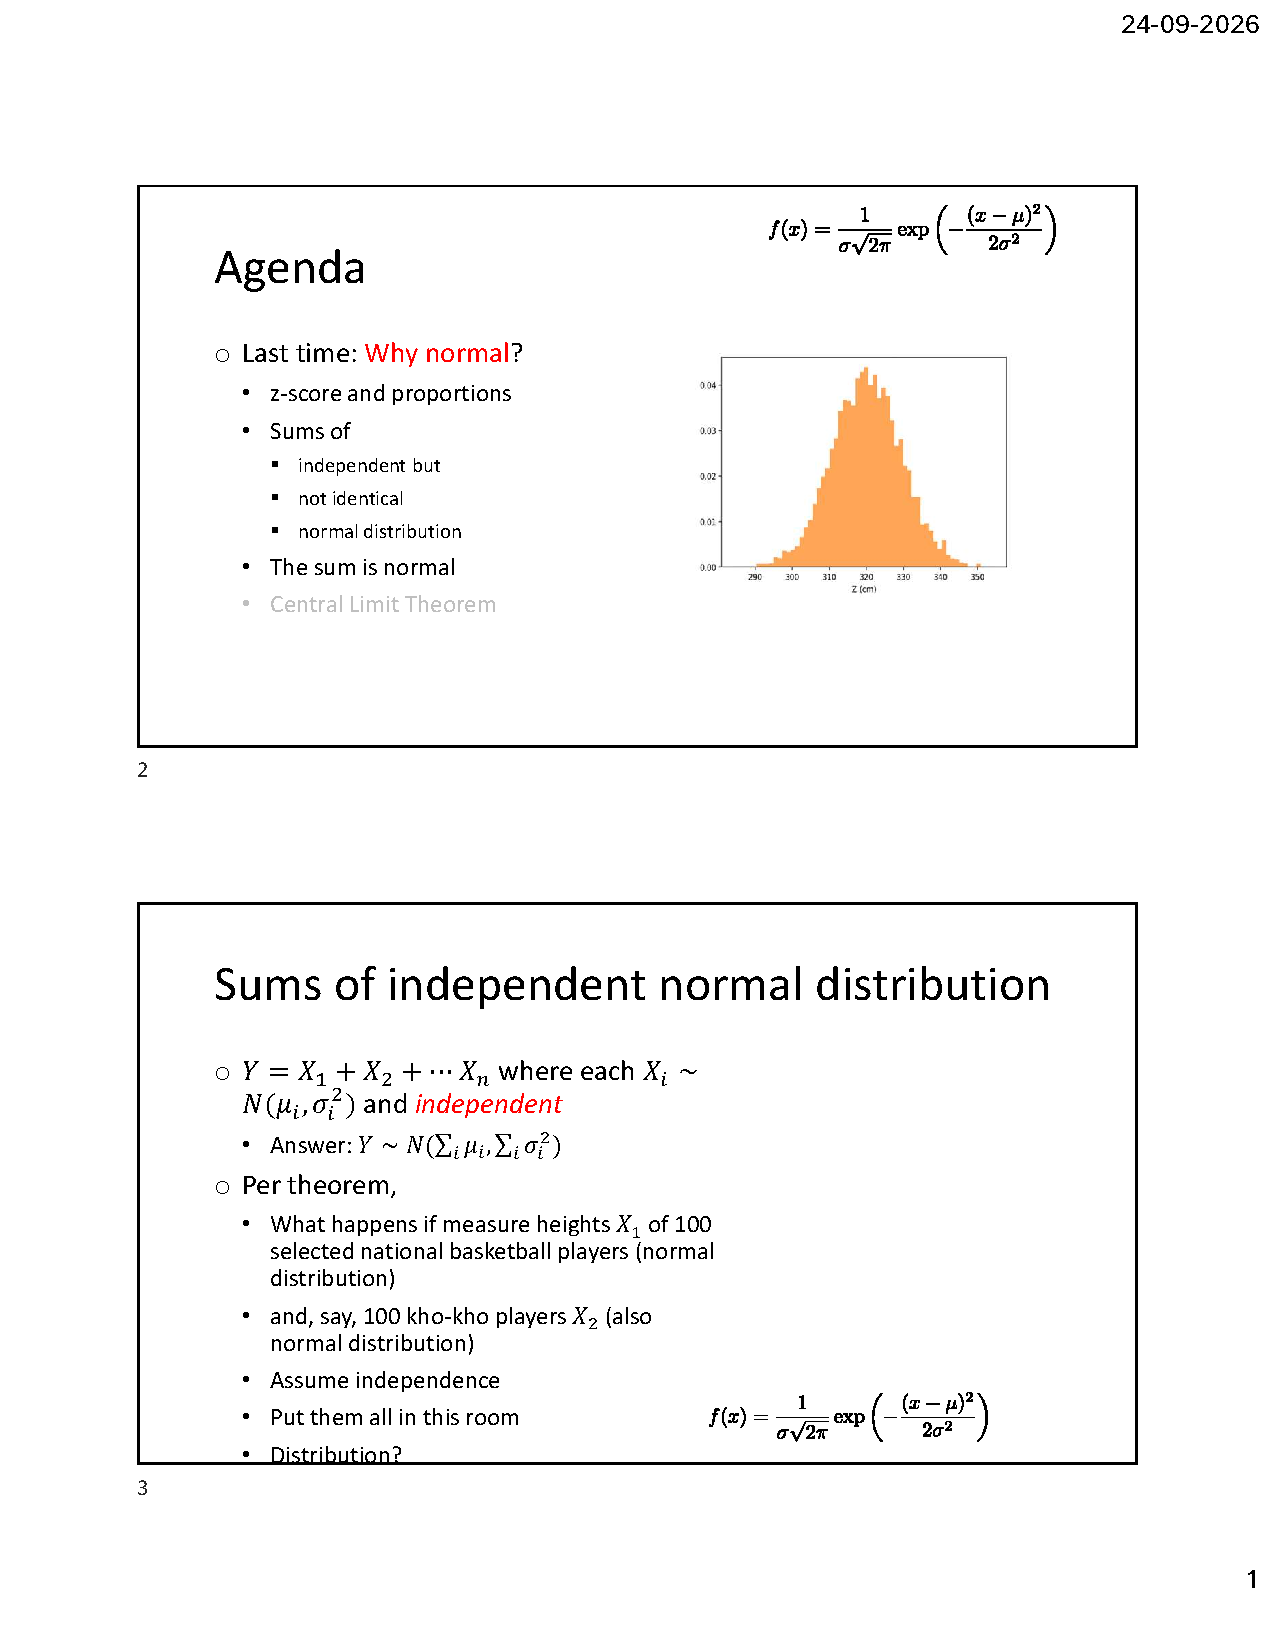
\includepdf[pages=-]{Lec19.pdf}
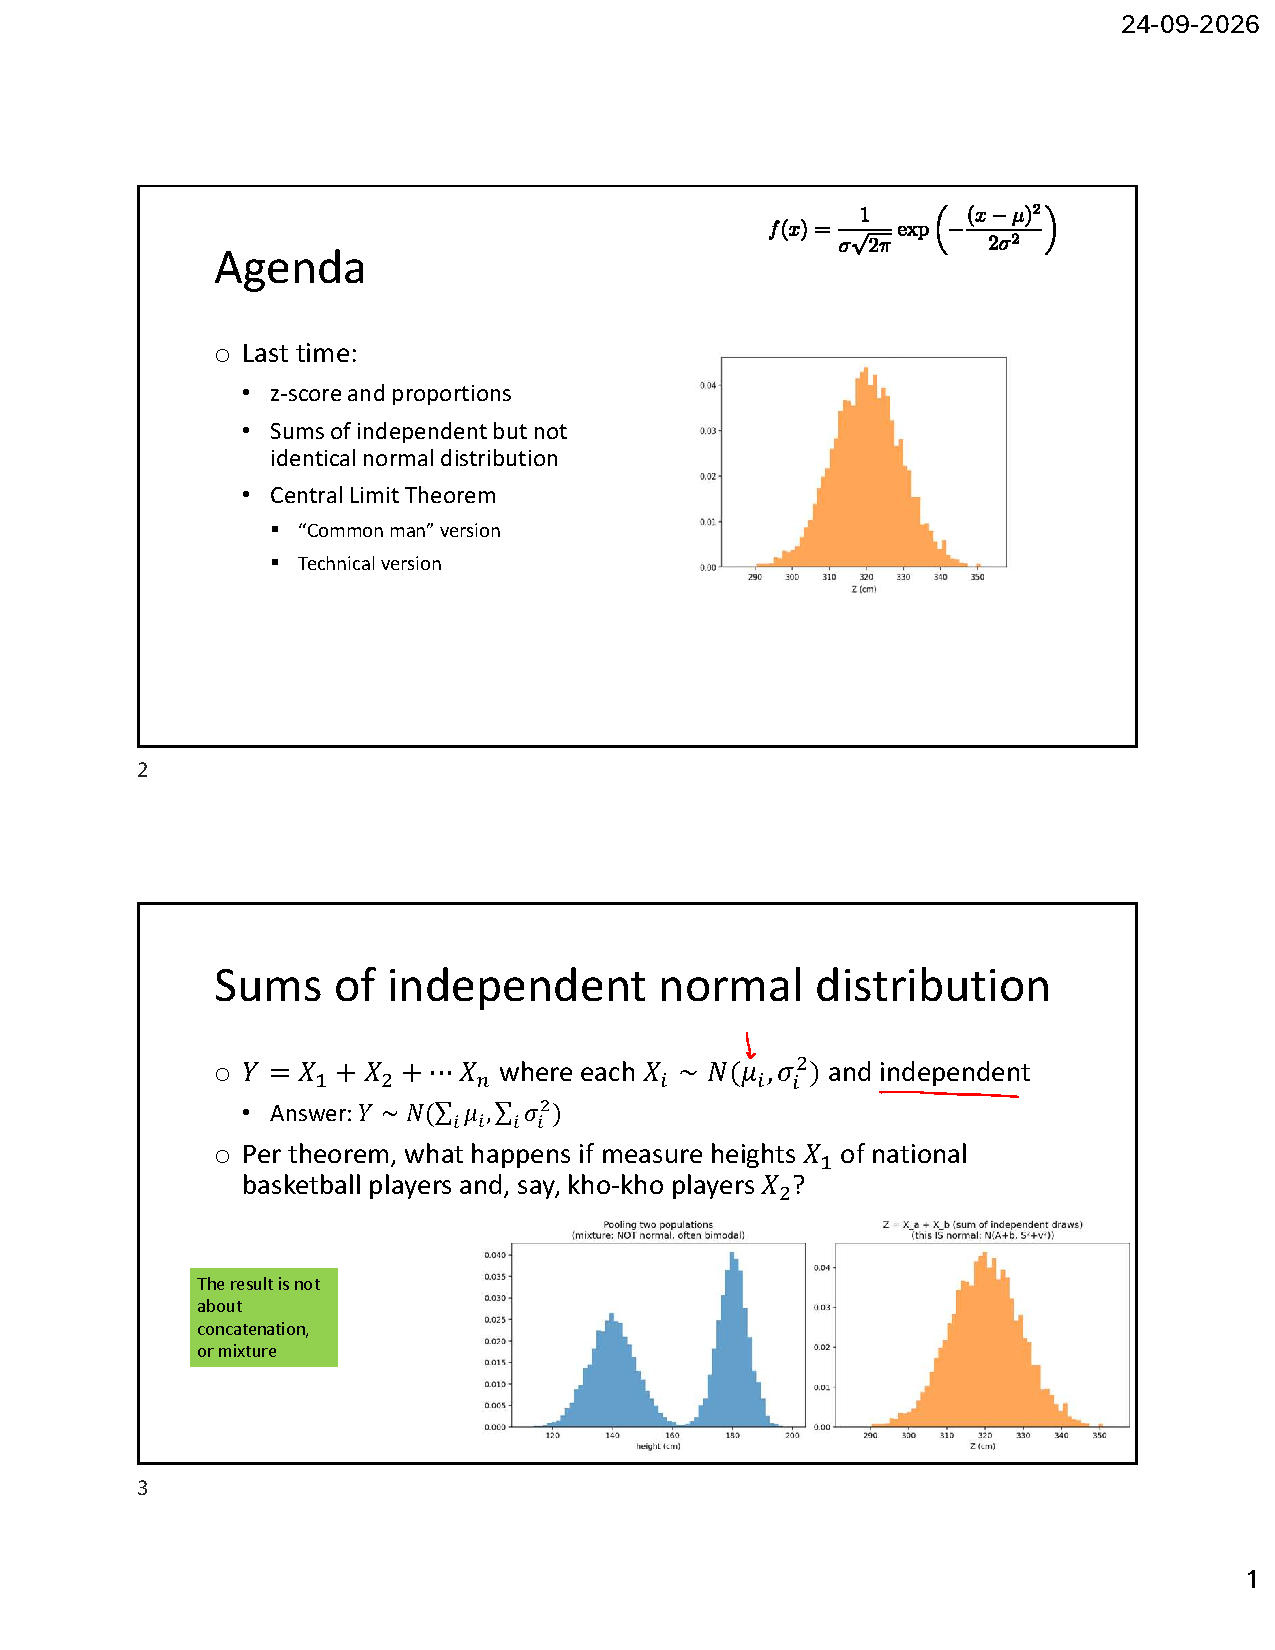
\includepdf[pages=-]{Lec21.pdf}
}




\subsection{Estimators, Distribution of sample mean, CLT for proportion}
{
\setbeamercolor{background canvas}{bg=} 
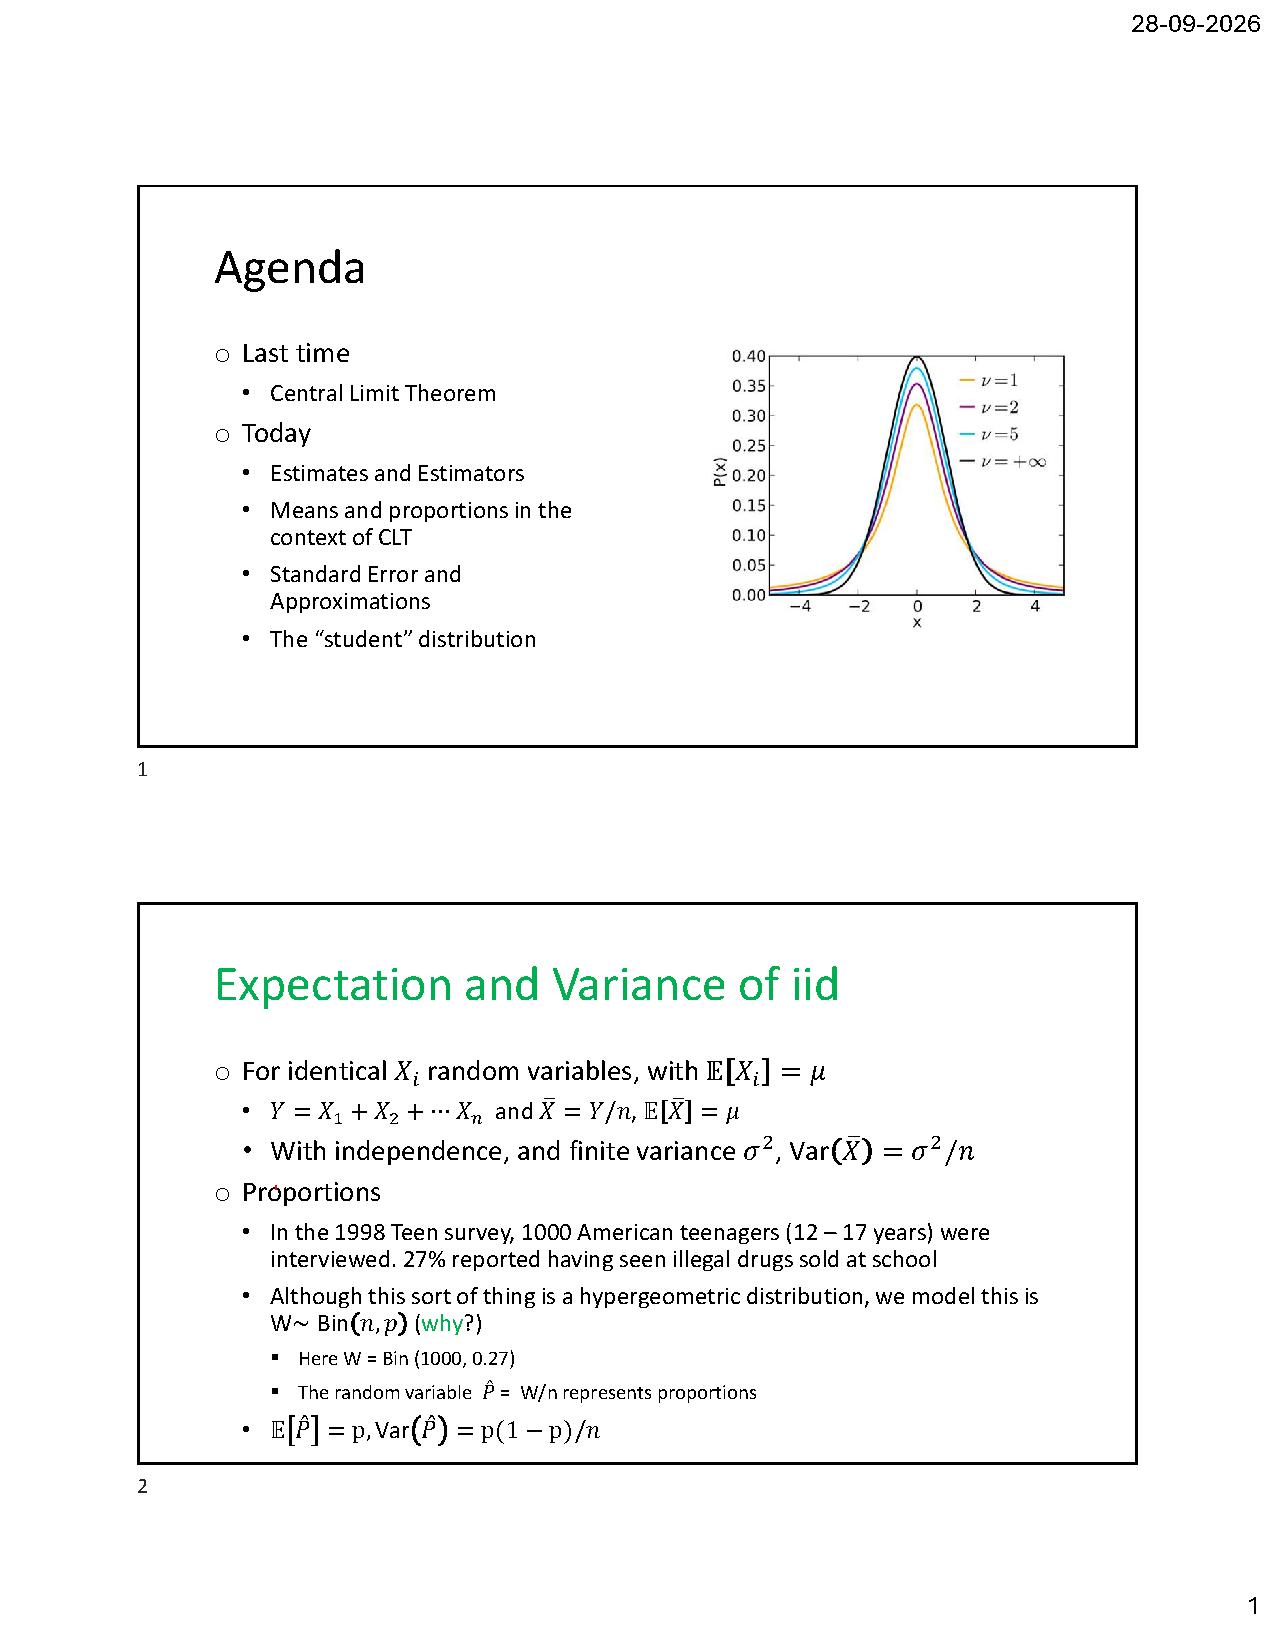
\includepdf[pages=-]{Lec28.pdf}
}

\subsection{Student's t distribution, Chi-square distribution}
{
\setbeamercolor{background canvas}{bg=} 
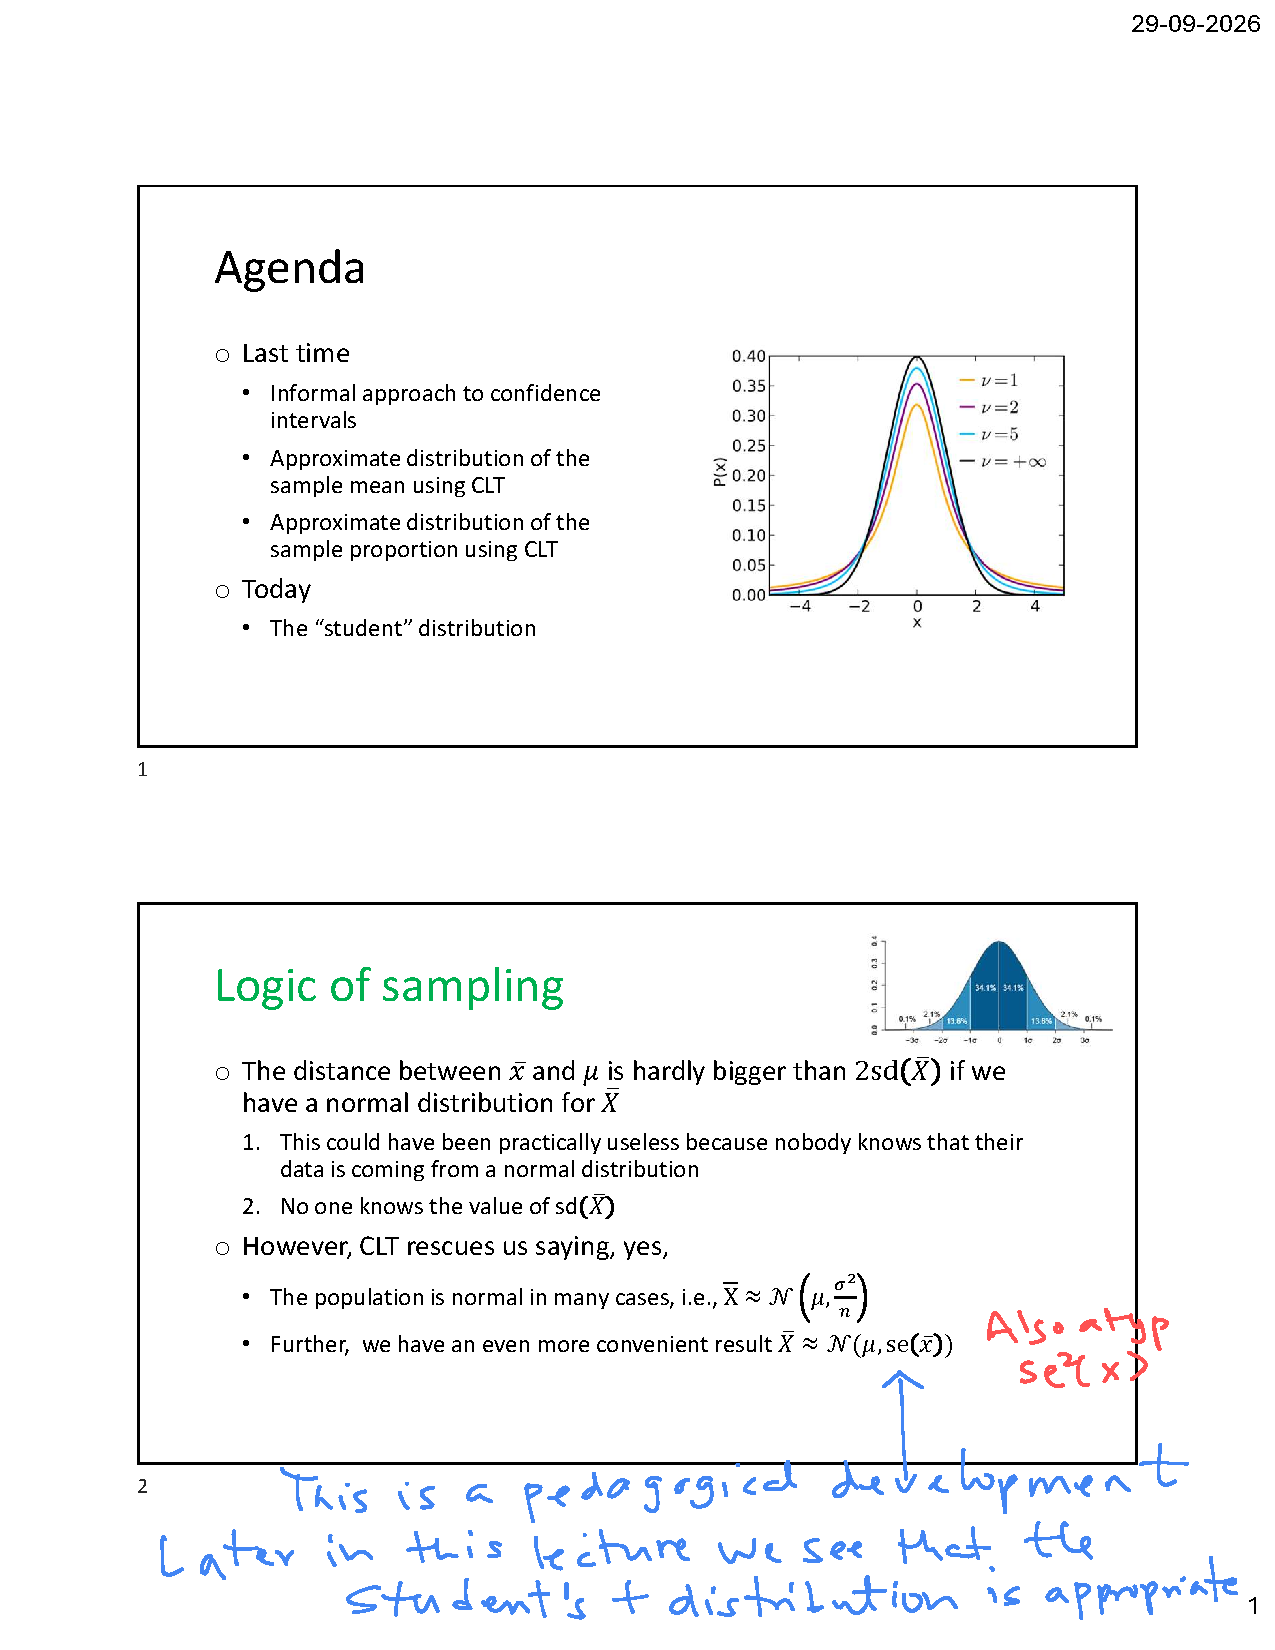
\includepdf[pages=-]{Lec29.pdf}
}
\section{Testing Confidence, Likelihood and Regression}
\subsection{Confidence intervals, Intro to Bias and Precision}
{
\setbeamercolor{background canvas}{bg=} 
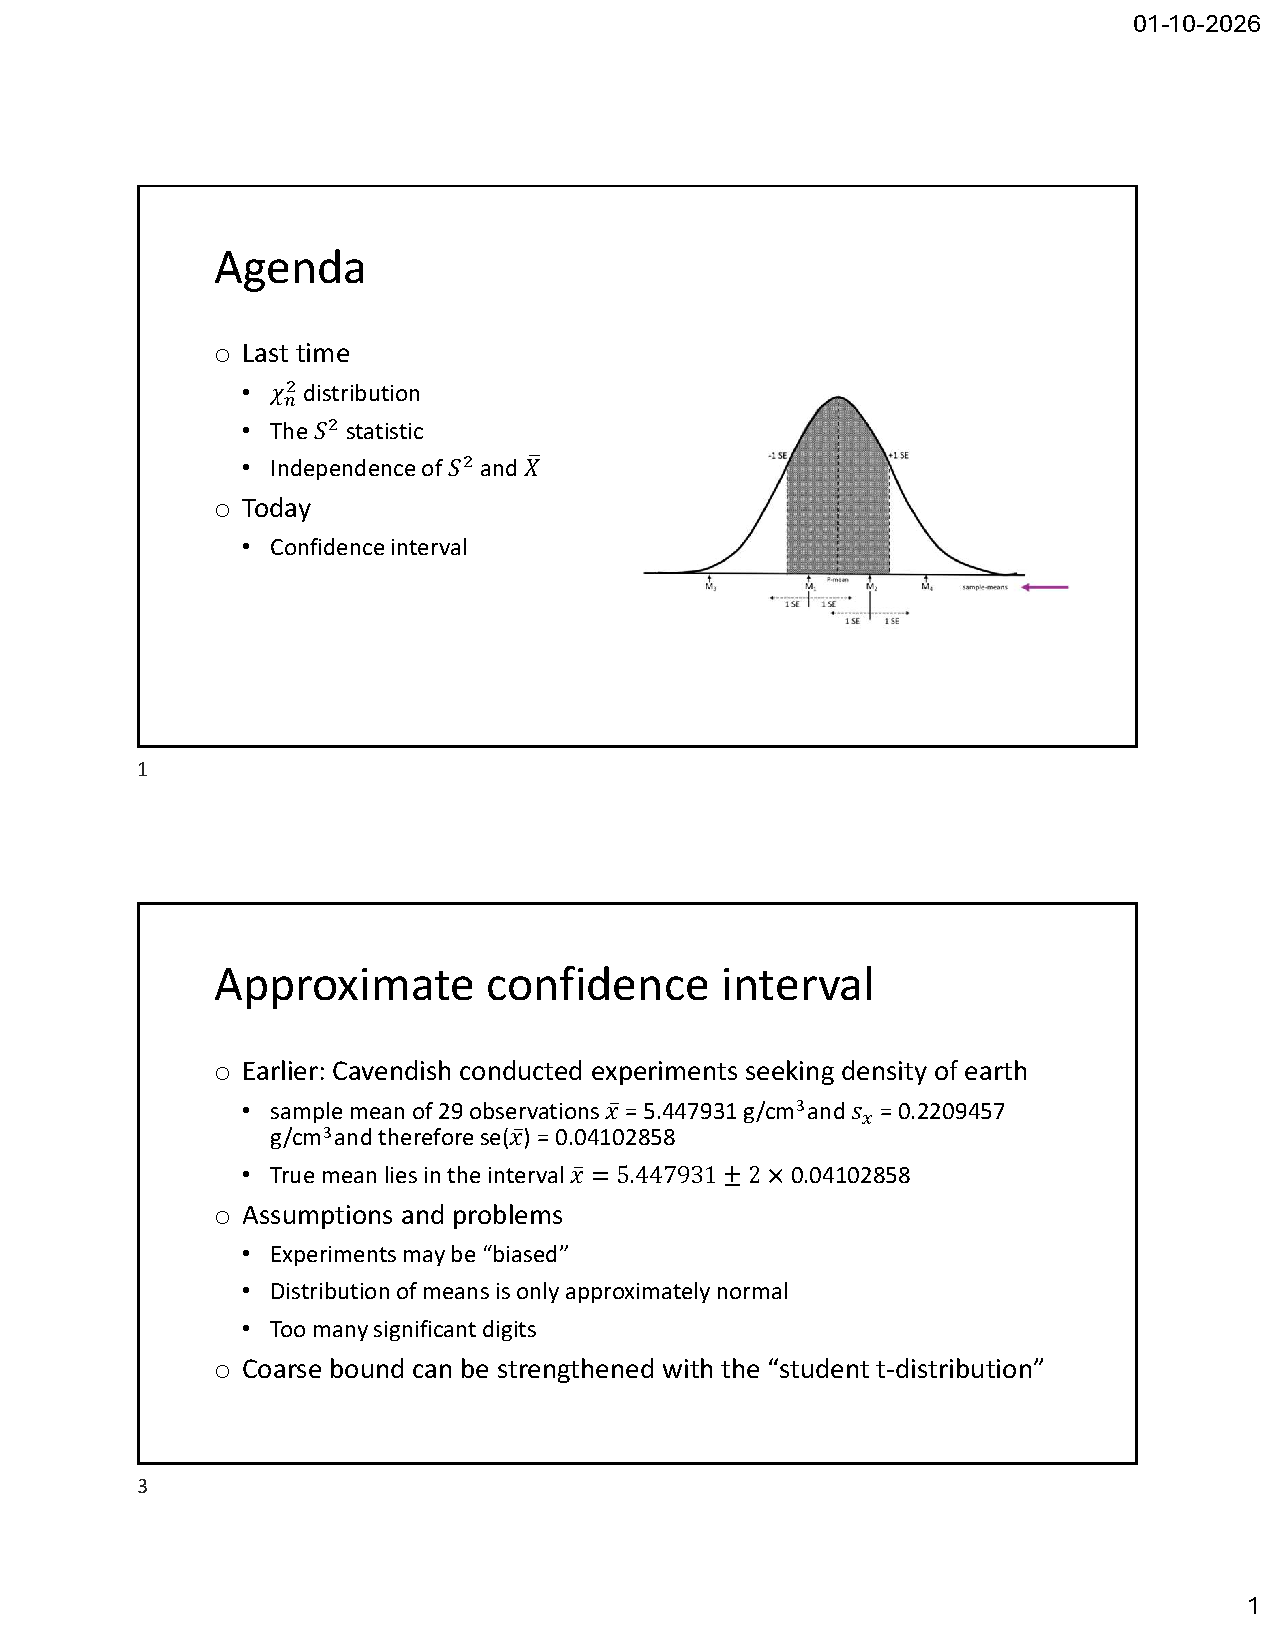
\includepdf[pages=-]{Lec30.pdf}
}

\subsection{Hypothesis Testing}
{
\setbeamercolor{background canvas}{bg=} 
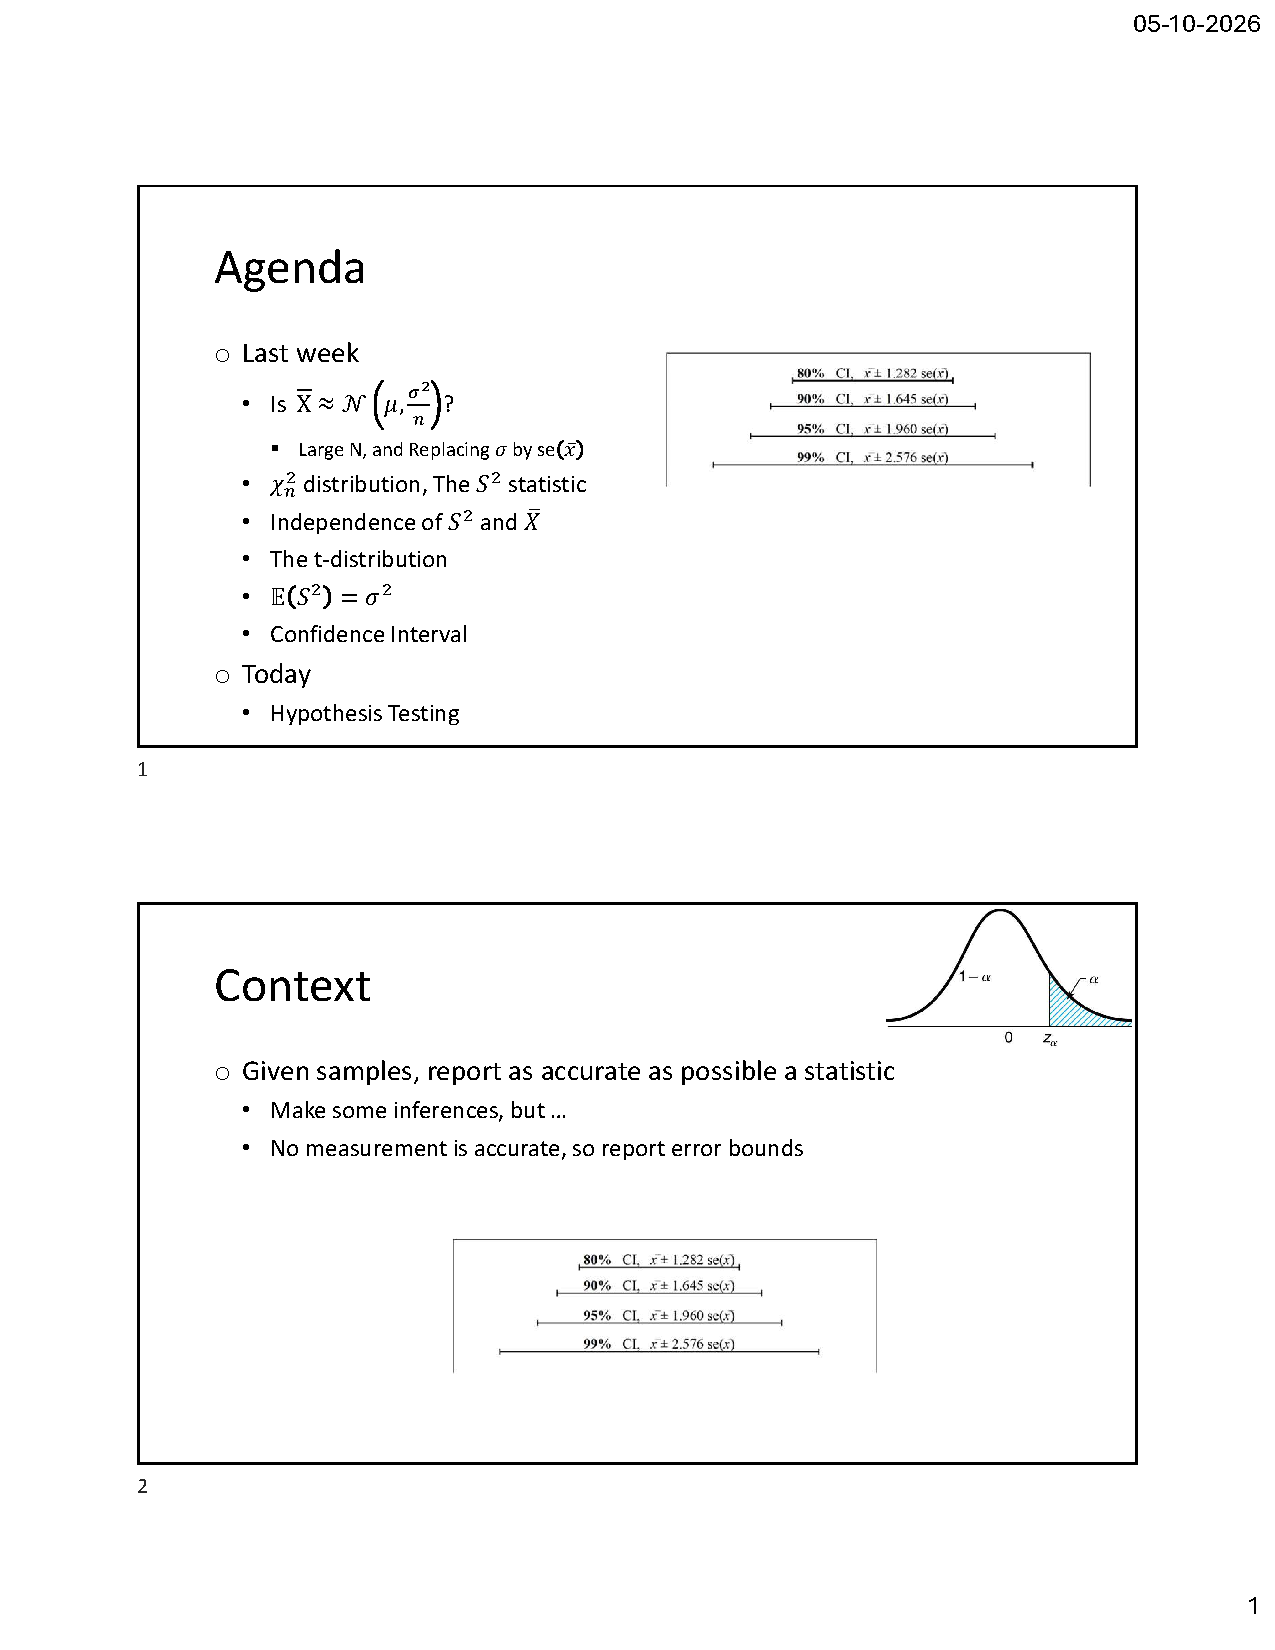
\includepdf[pages=-]{Lec31.pdf}
}

\subsection{Parameter Estimation, MLE}
{
\setbeamercolor{background canvas}{bg=} 
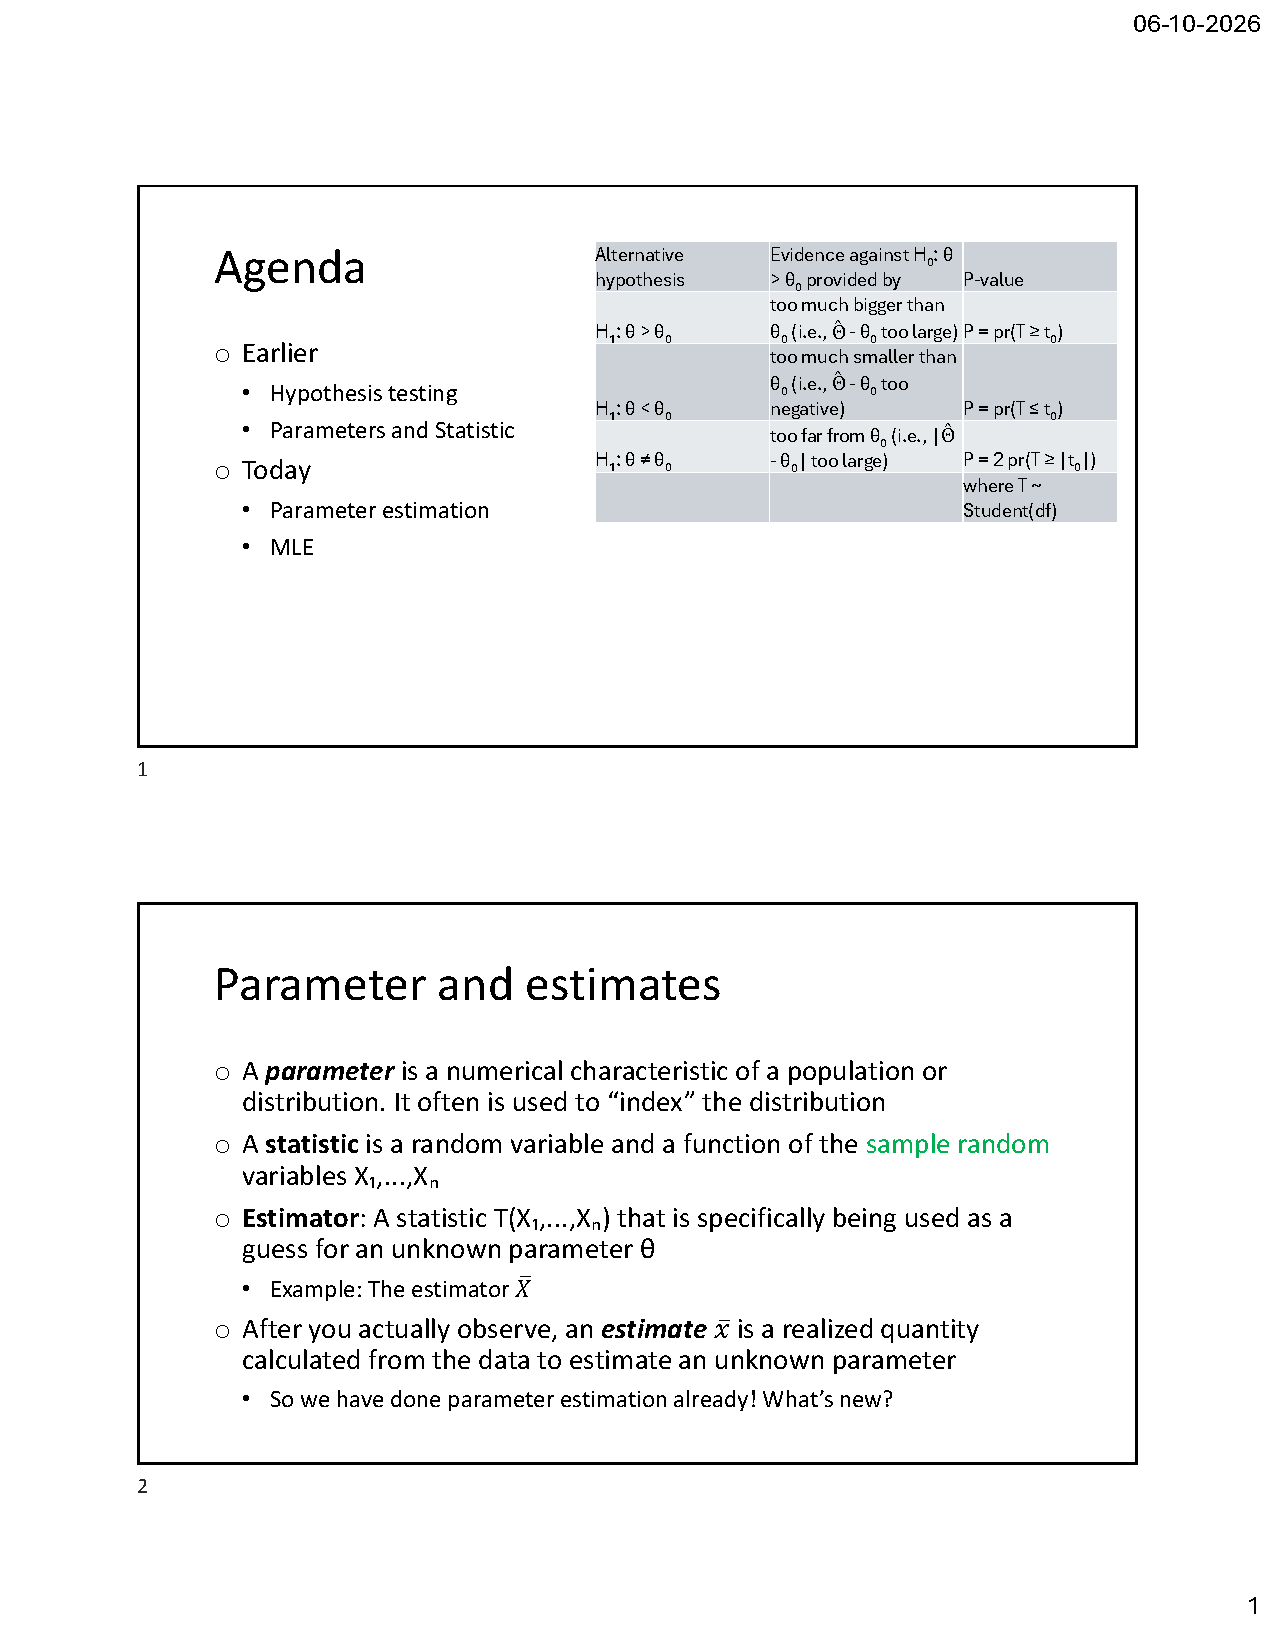
\includepdf[pages=-]{Lec32.pdf}
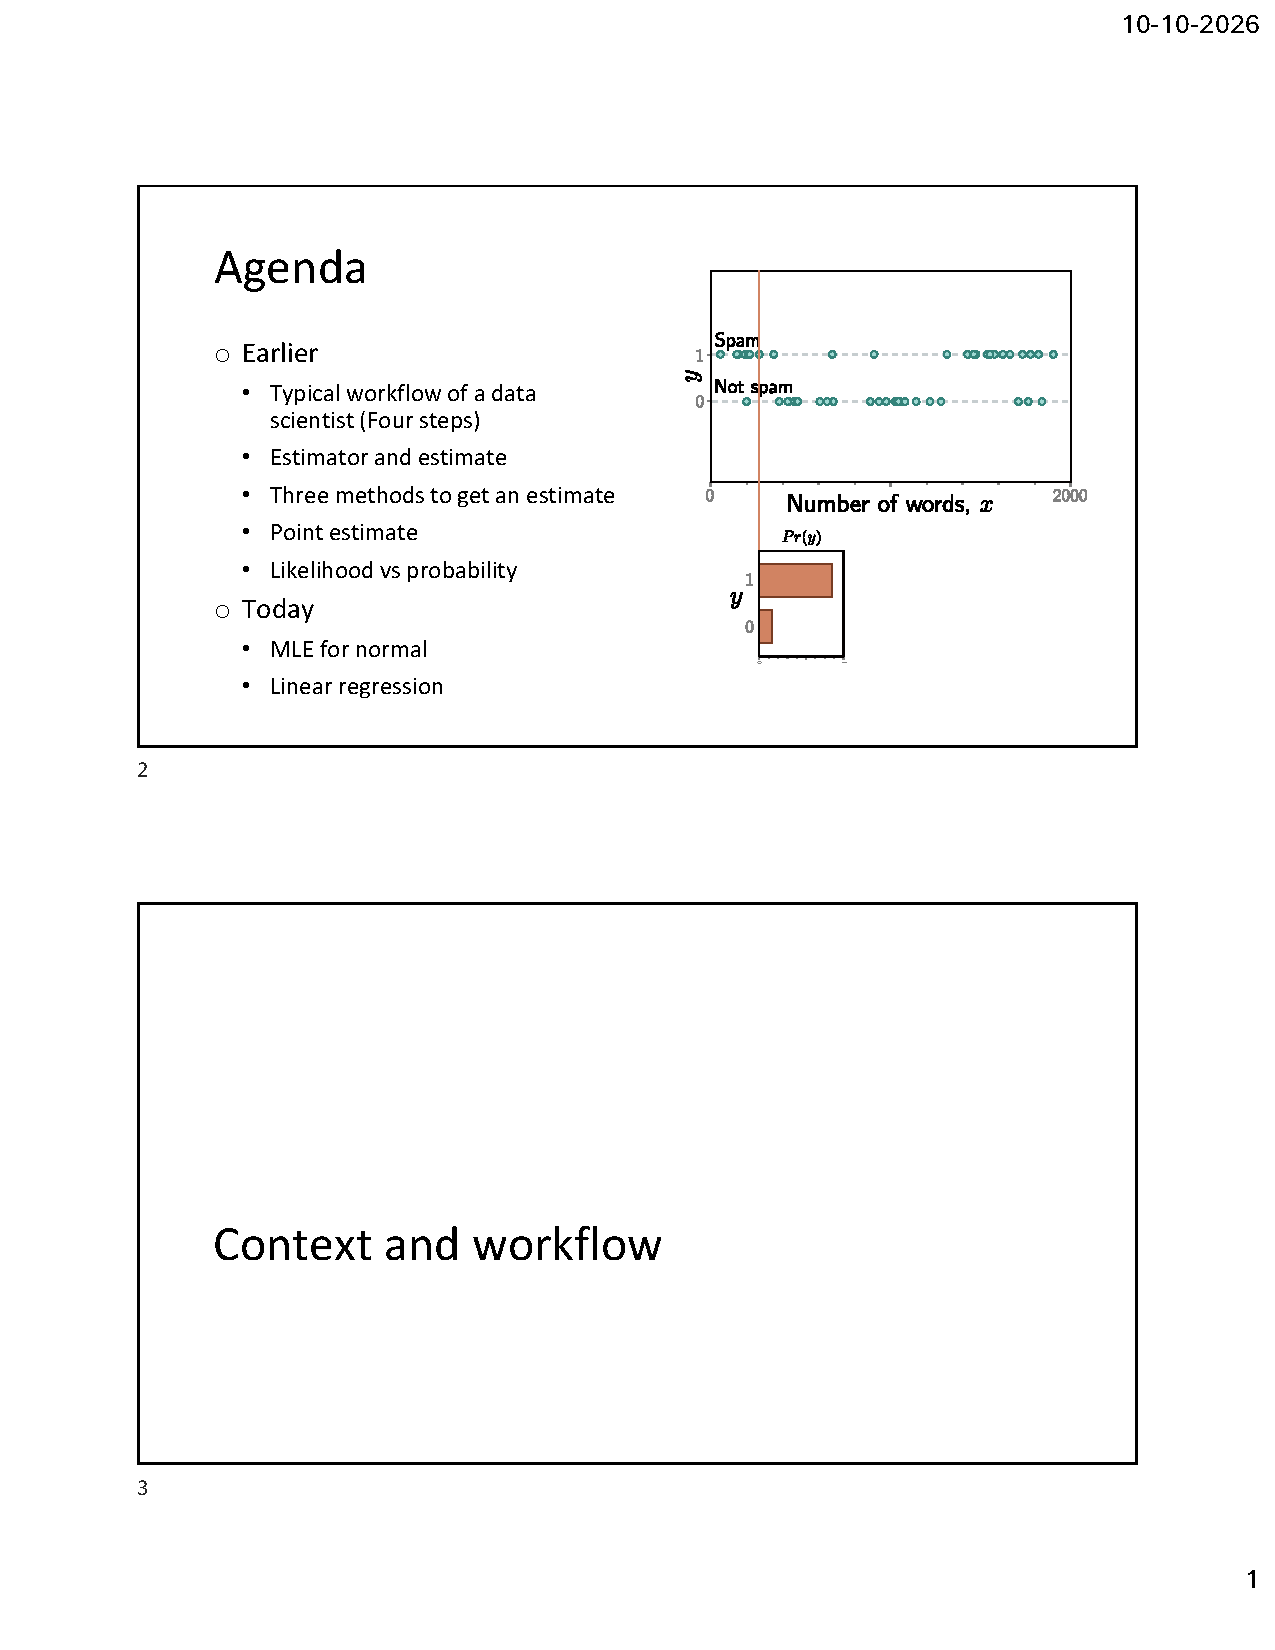
\includepdf[pages={1-6}]{Lec33.pdf}
}

\subsection{Linear Regression and Distribution of Estimators, Bias and Variance}
{
\setbeamercolor{background canvas}{bg=} 
\includepdf[pages={7-8}]{Lec33.pdf}
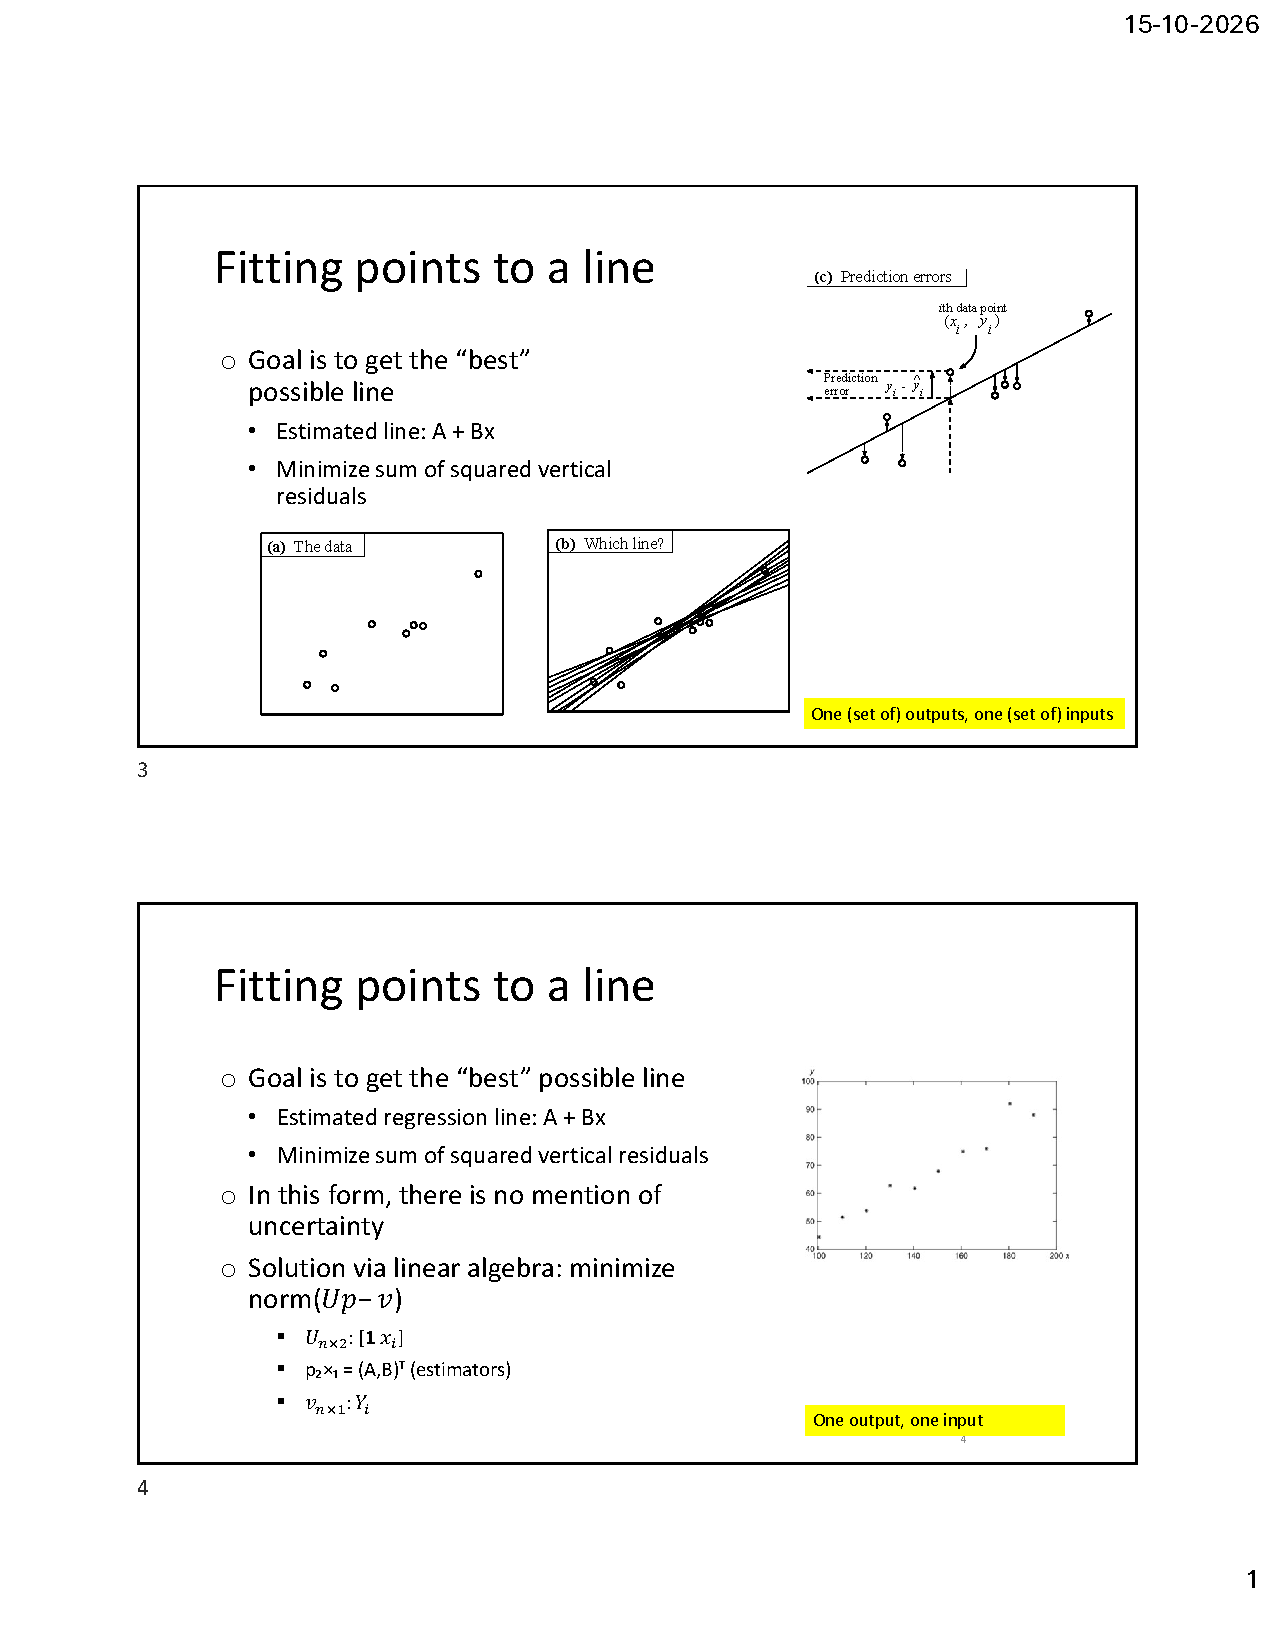
\includepdf[pages=-]{Lec34.pdf}
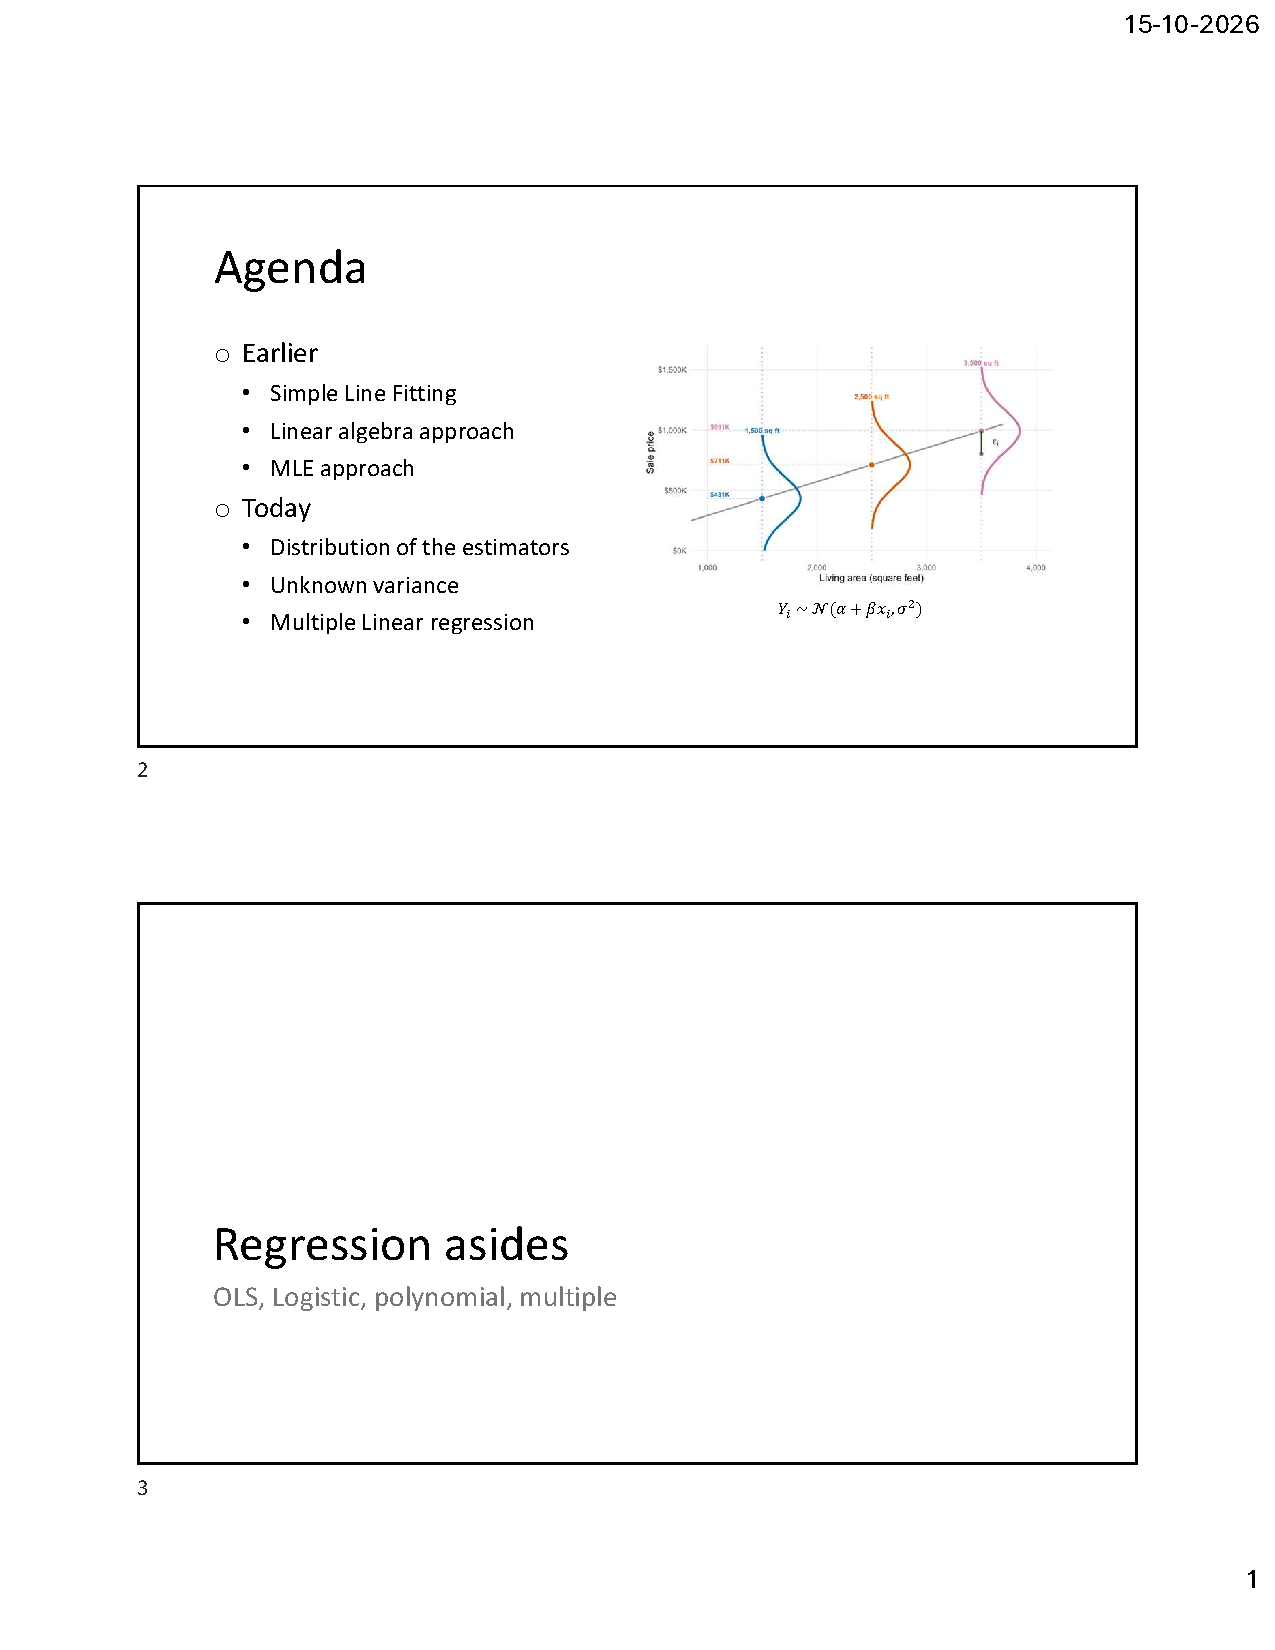
\includepdf[pages=-]{Lec35.pdf}
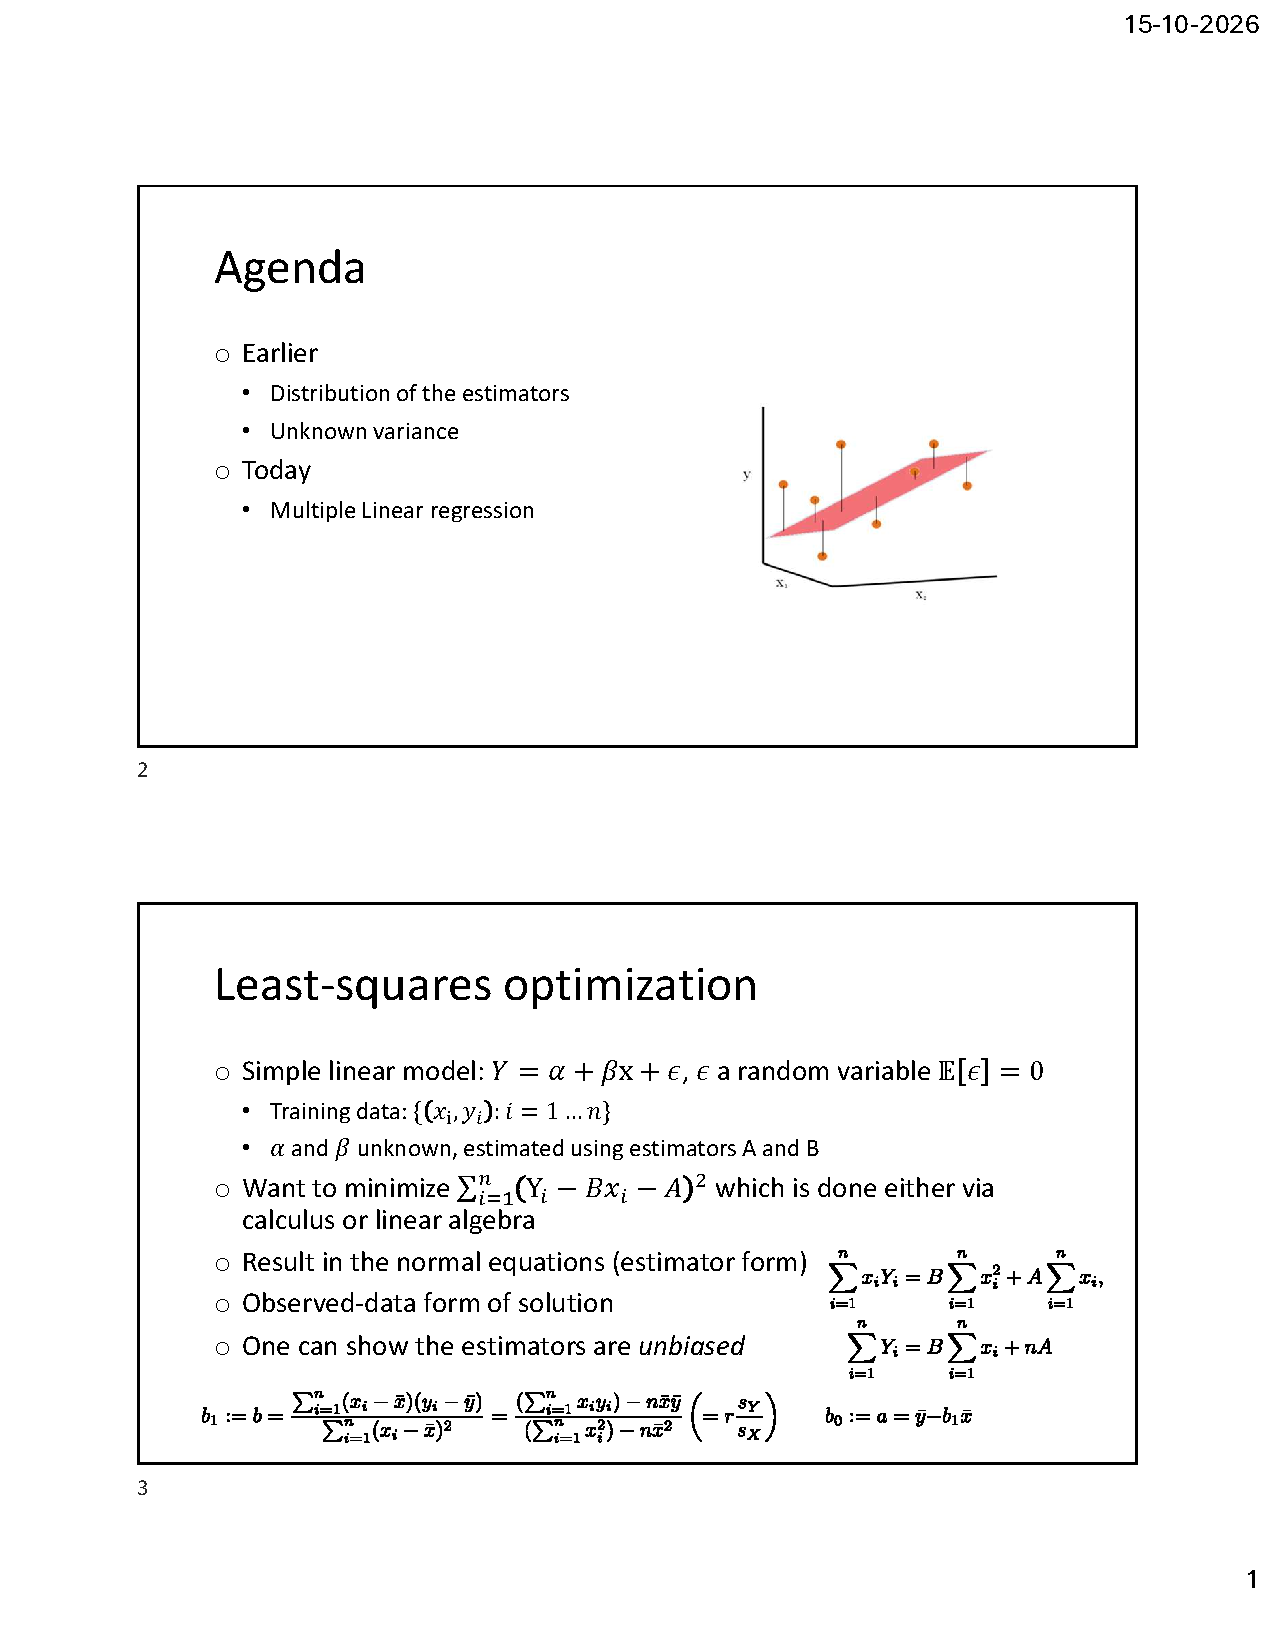
\includepdf[pages=-]{Lec36.pdf}
}


\subsection{Confidence Intervals and Multi-population comparison}
{
\setbeamercolor{background canvas}{bg=} 
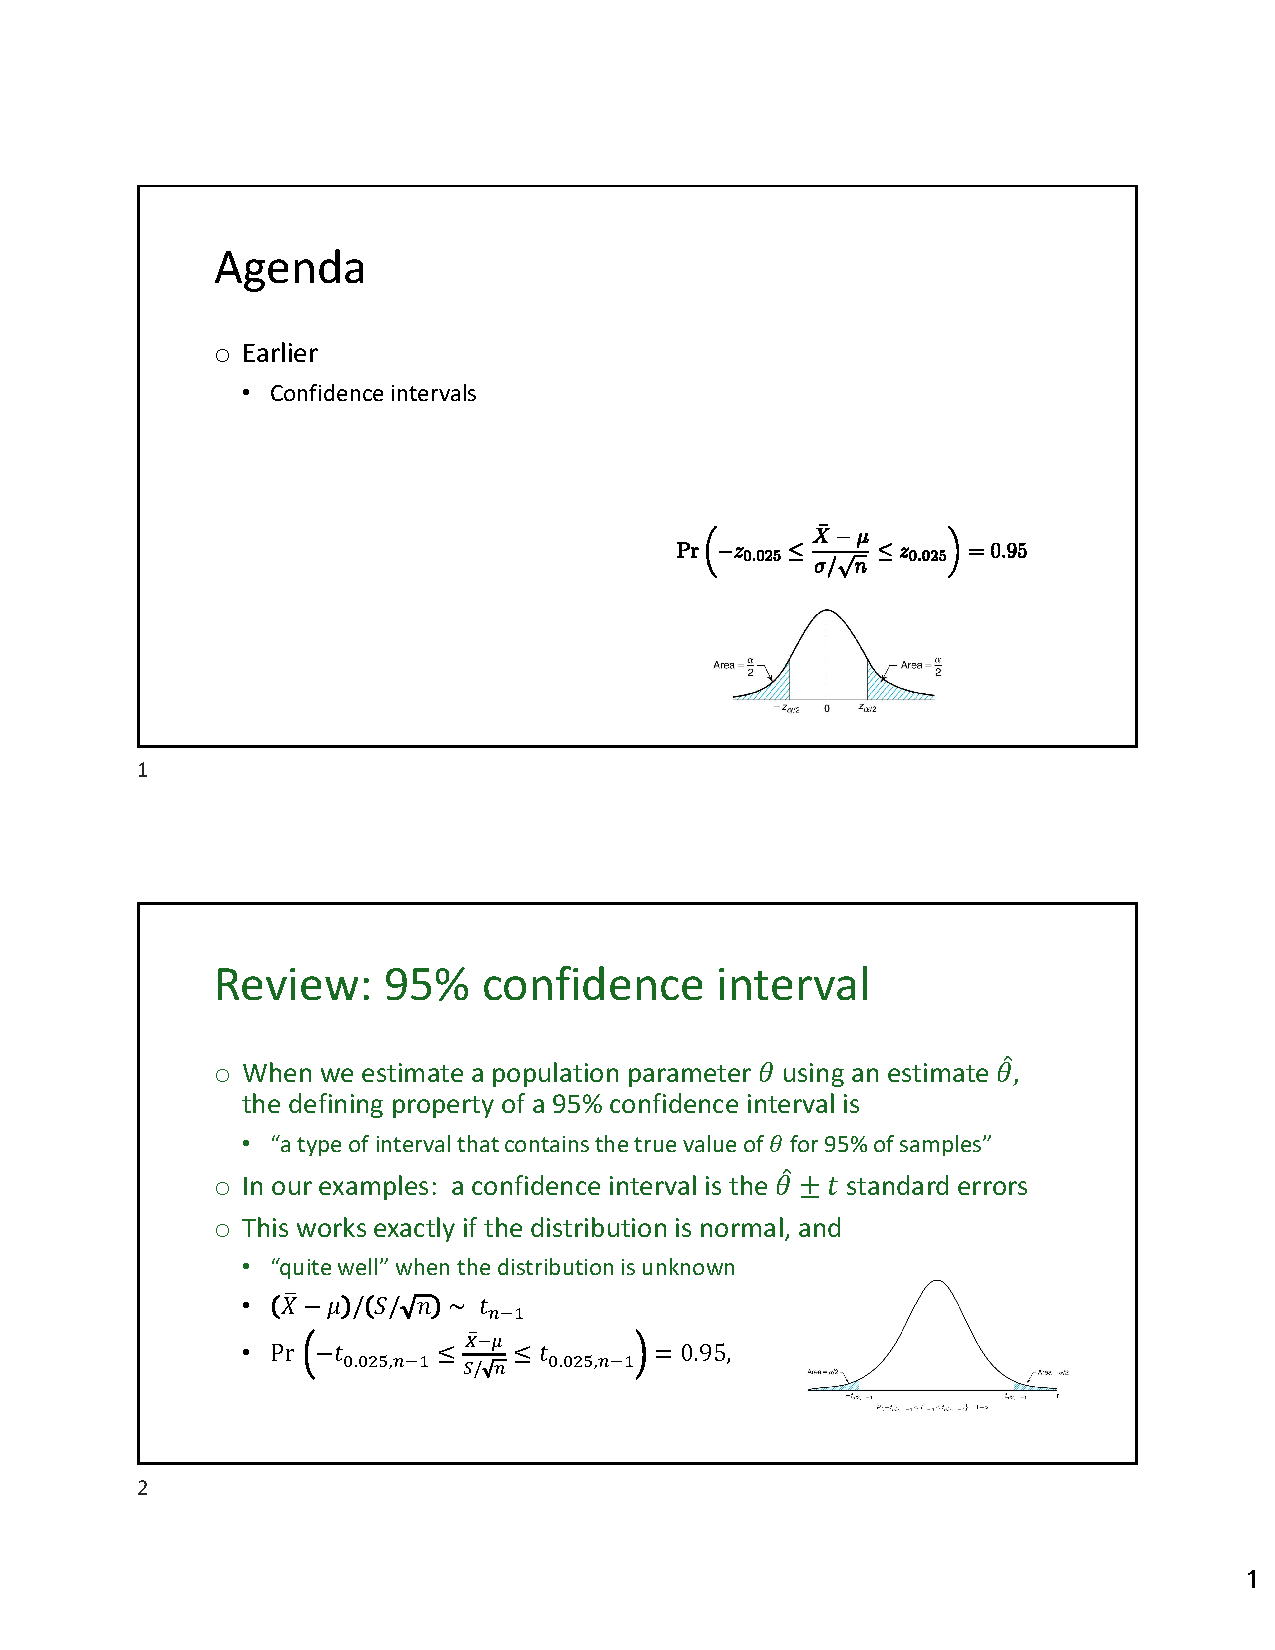
\includepdf[pages=-]{Lec37.pdf}
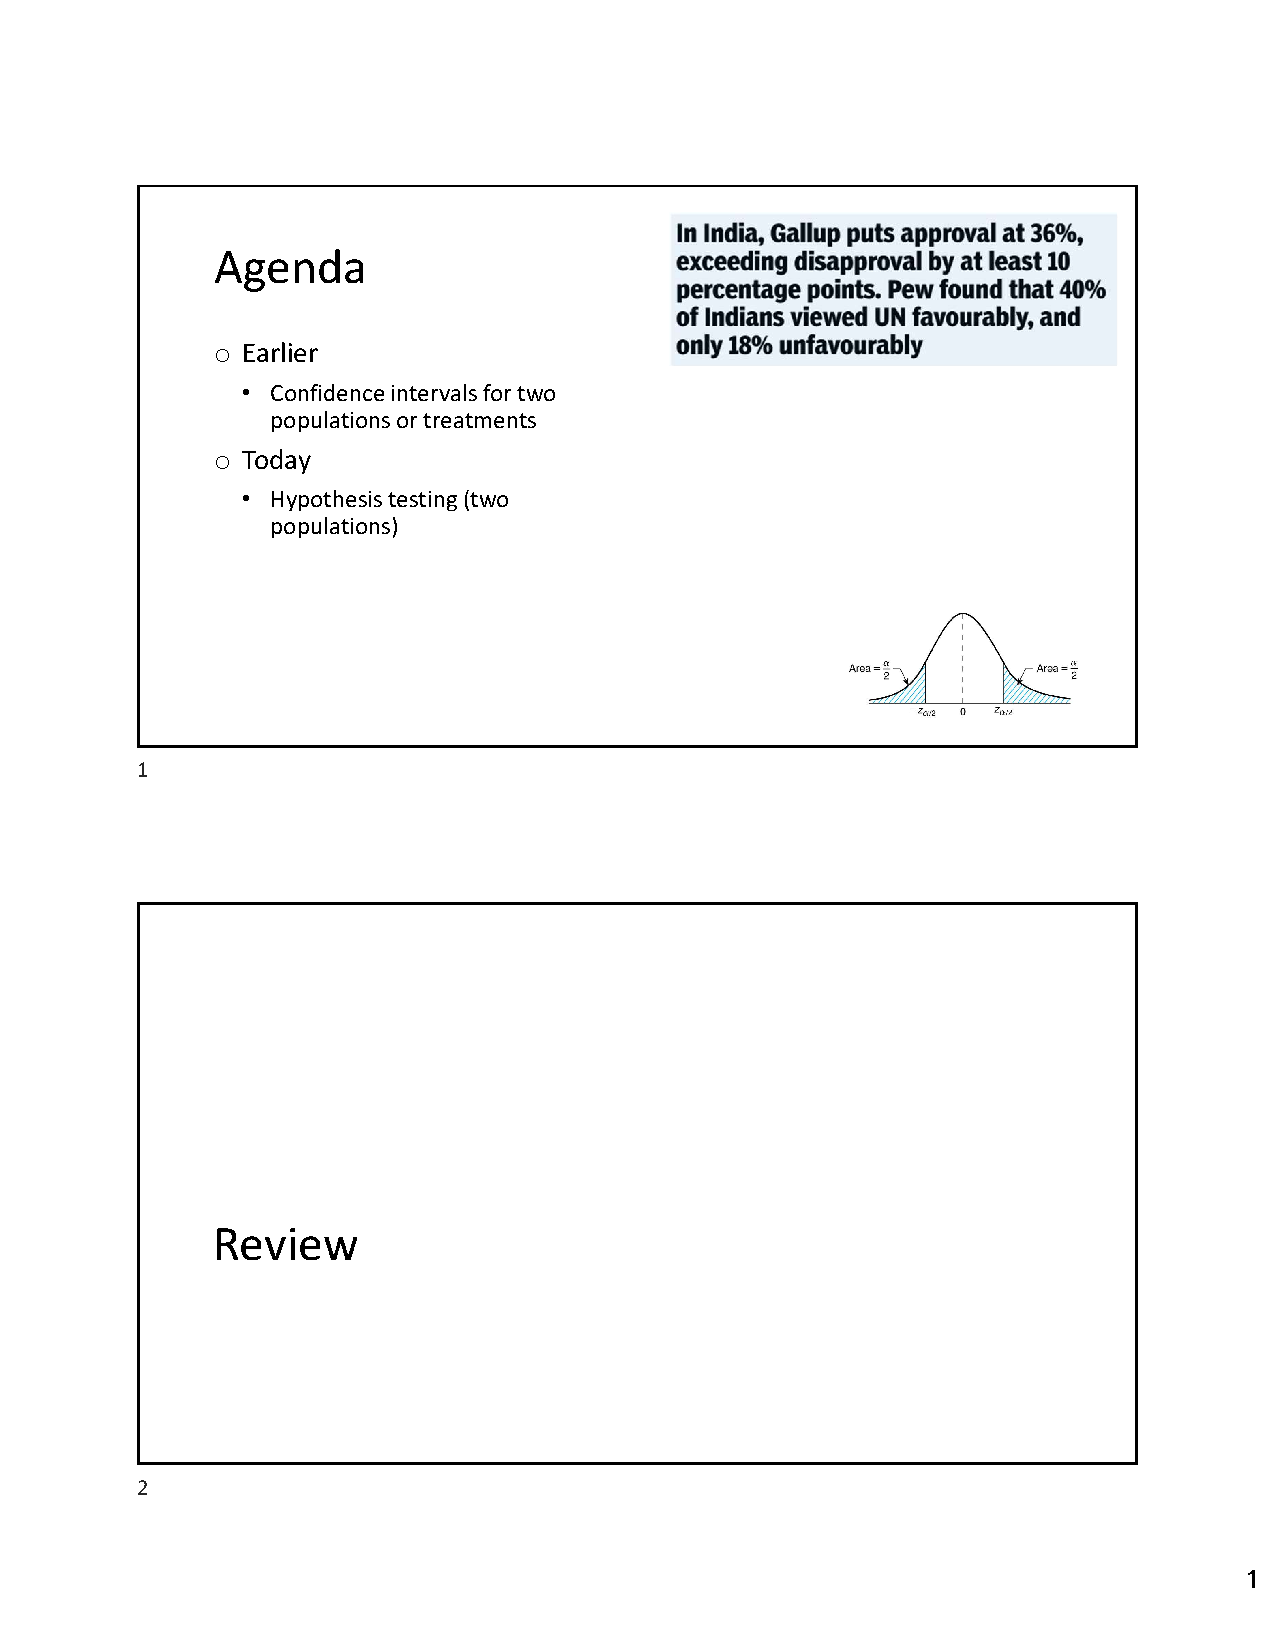
\includepdf[pages=-]{Lec39.pdf}
}


\subsection{Hypothesis Testing, Type1 and Type2 Error}
{
\setbeamercolor{background canvas}{bg=} 
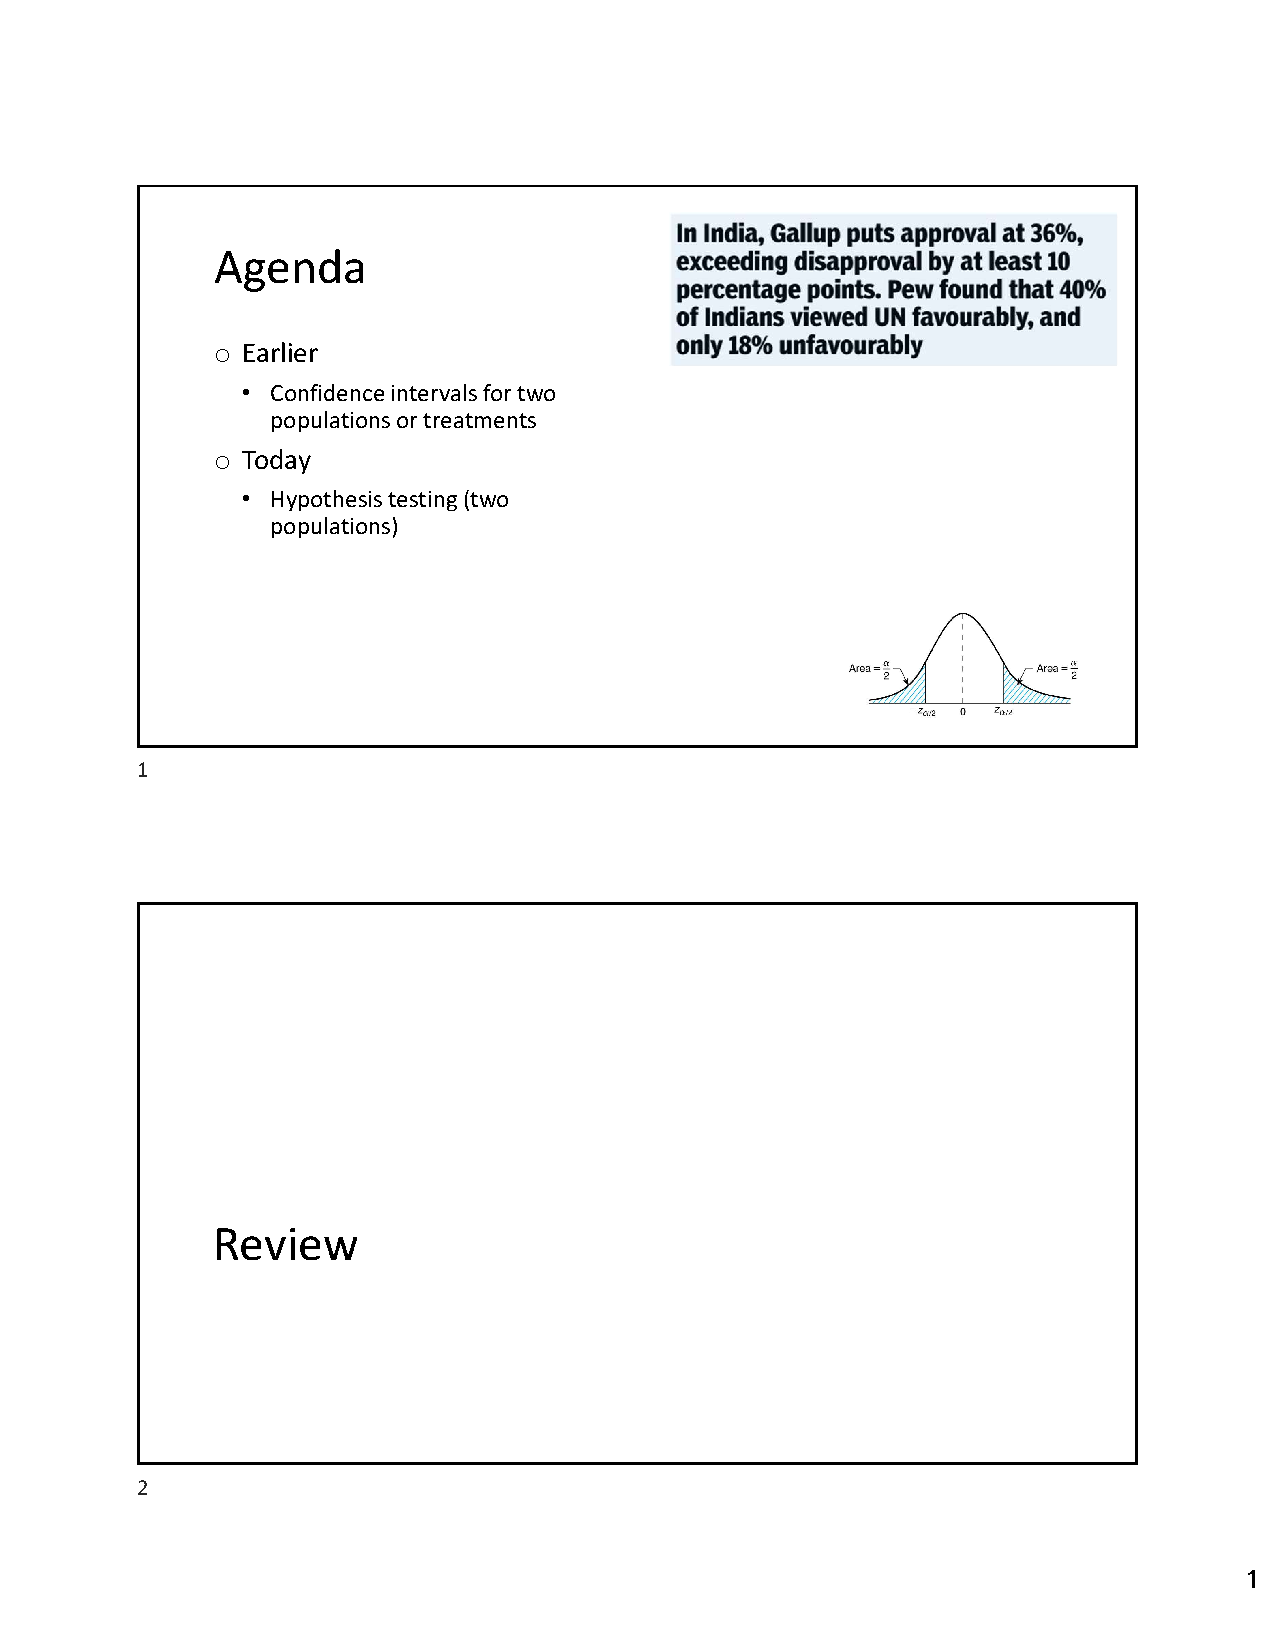
\includepdf[pages=-]{Lec40.pdf}
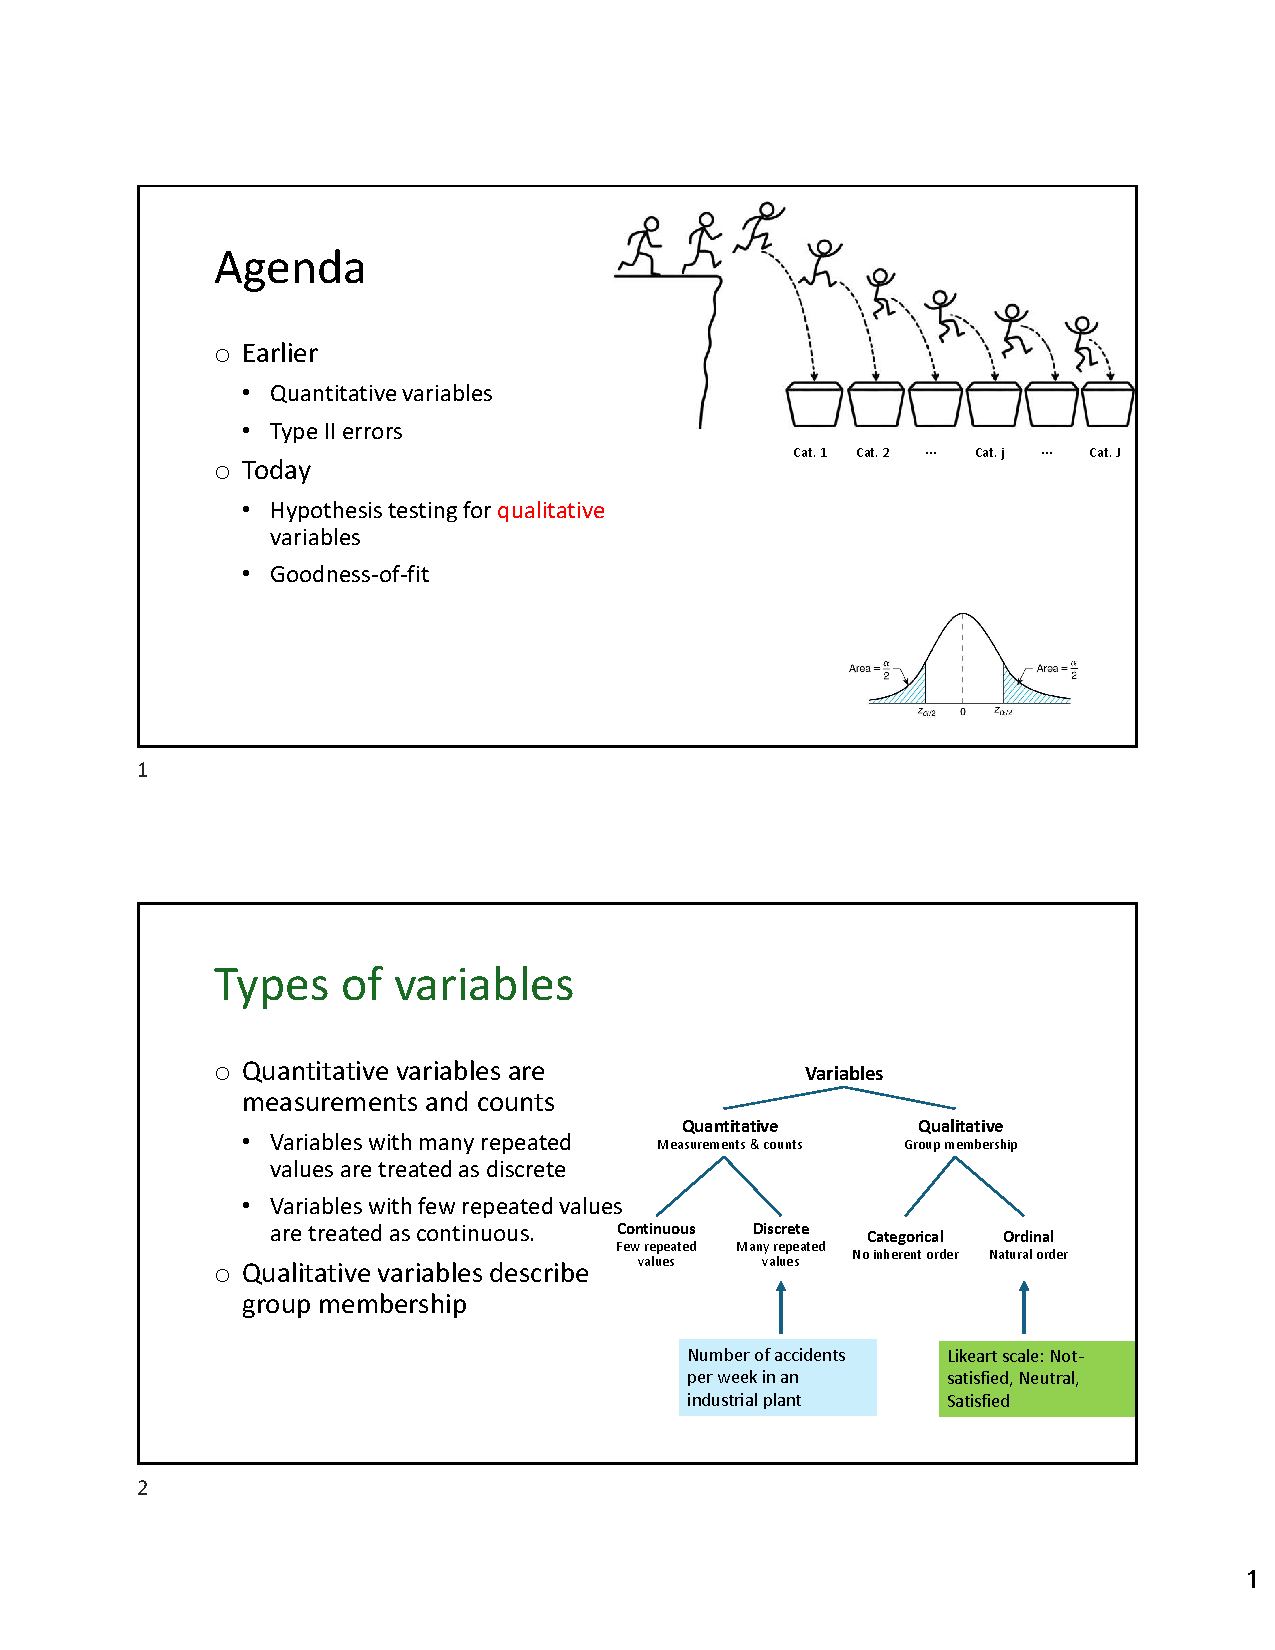
\includepdf[pages=-]{Lec41.pdf}
}


\subsection{Goodness of Fit}
{
\setbeamercolor{background canvas}{bg=} 
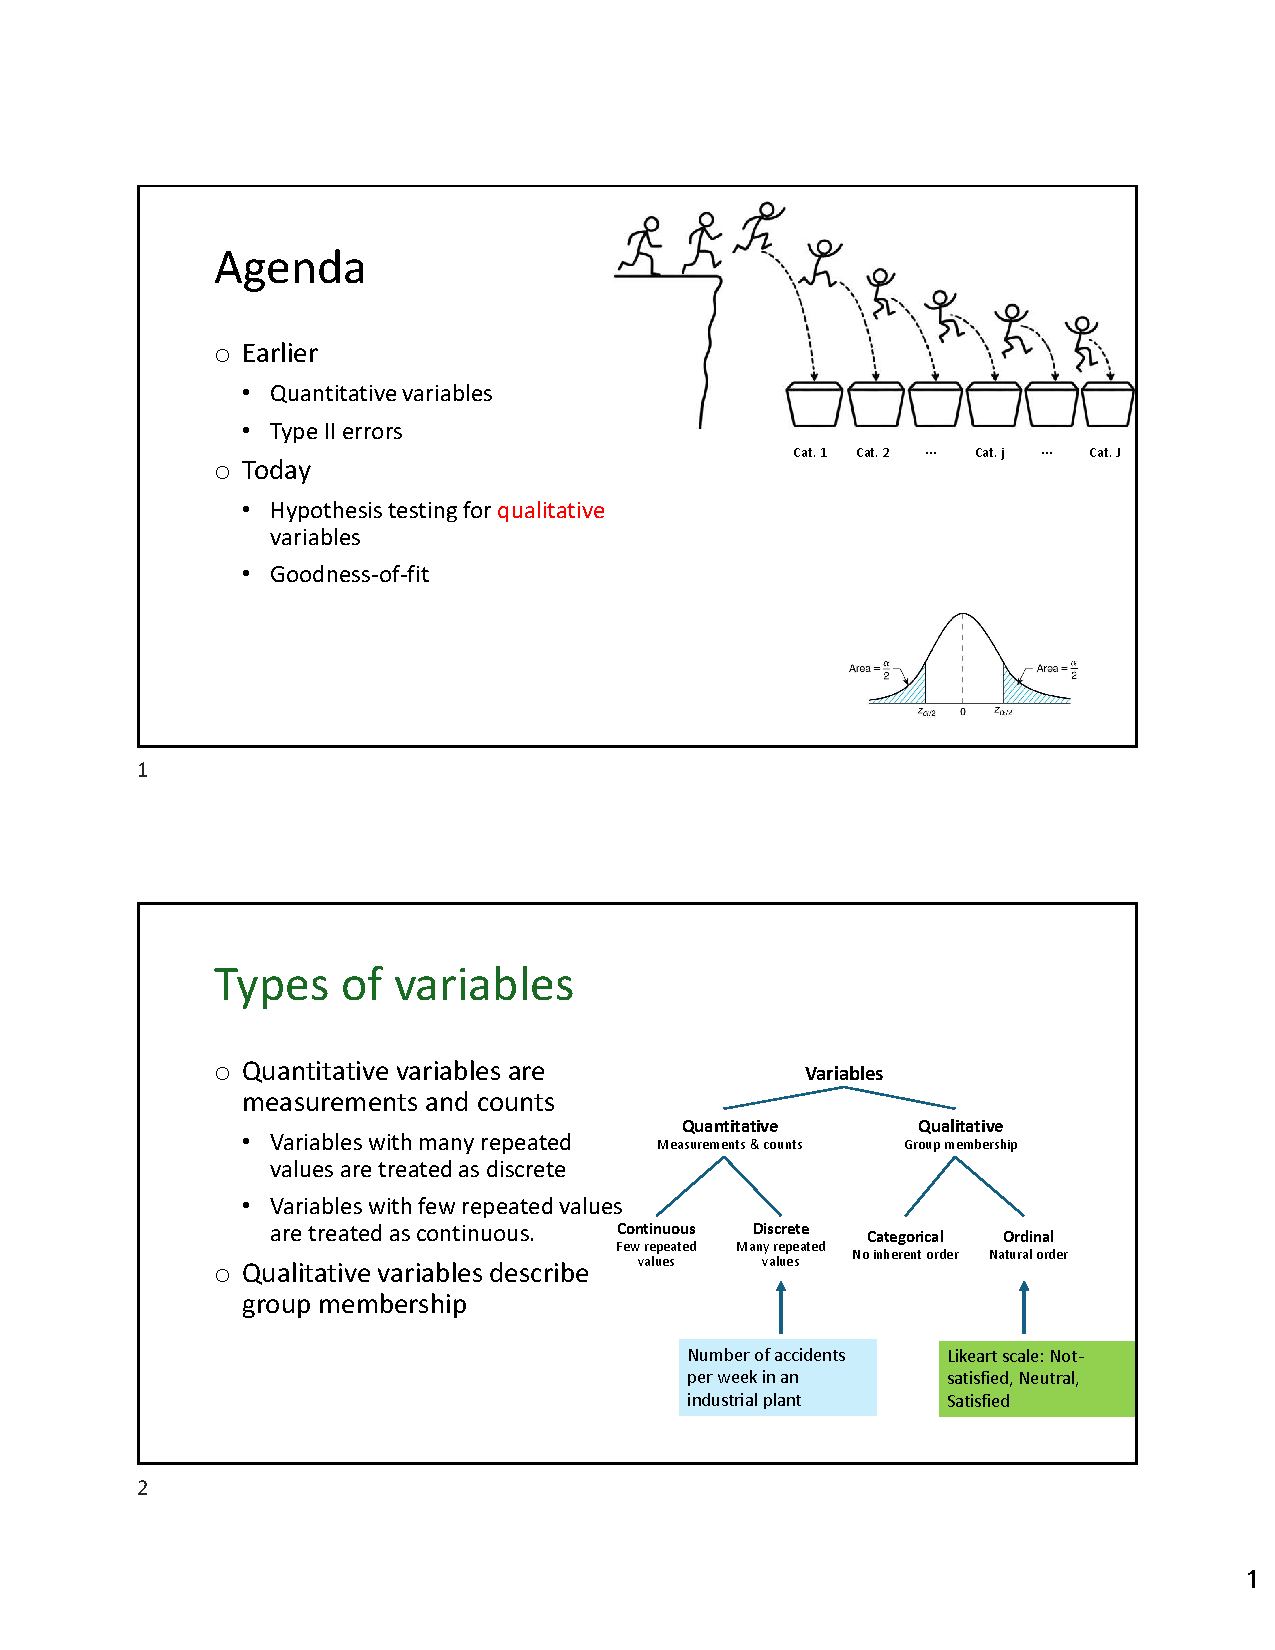
\includepdf[pages=-]{Lec42.pdf}
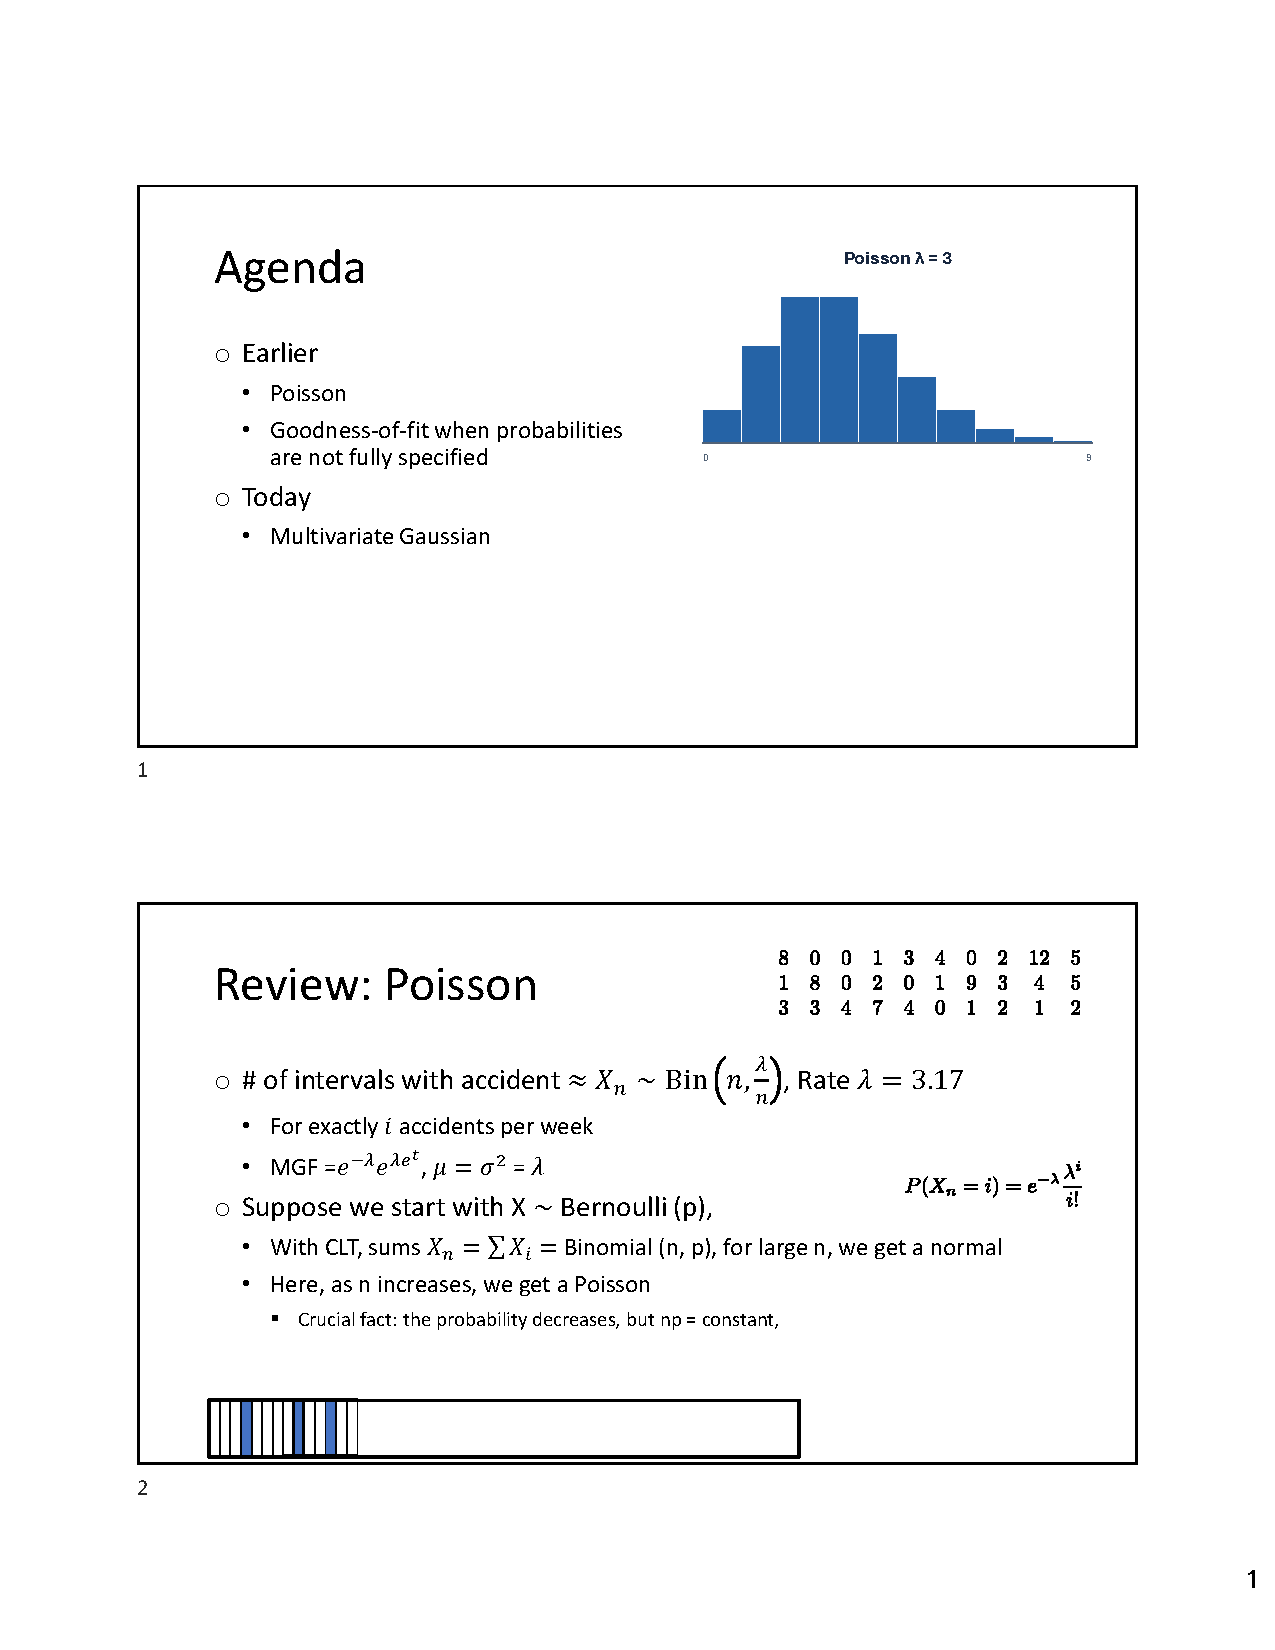
\includepdf[pages=-]{Lec43.pdf}
}
\section{More for ML Course}
\subsection{Multivariate gaussian}
{
\setbeamercolor{background canvas}{bg=} 
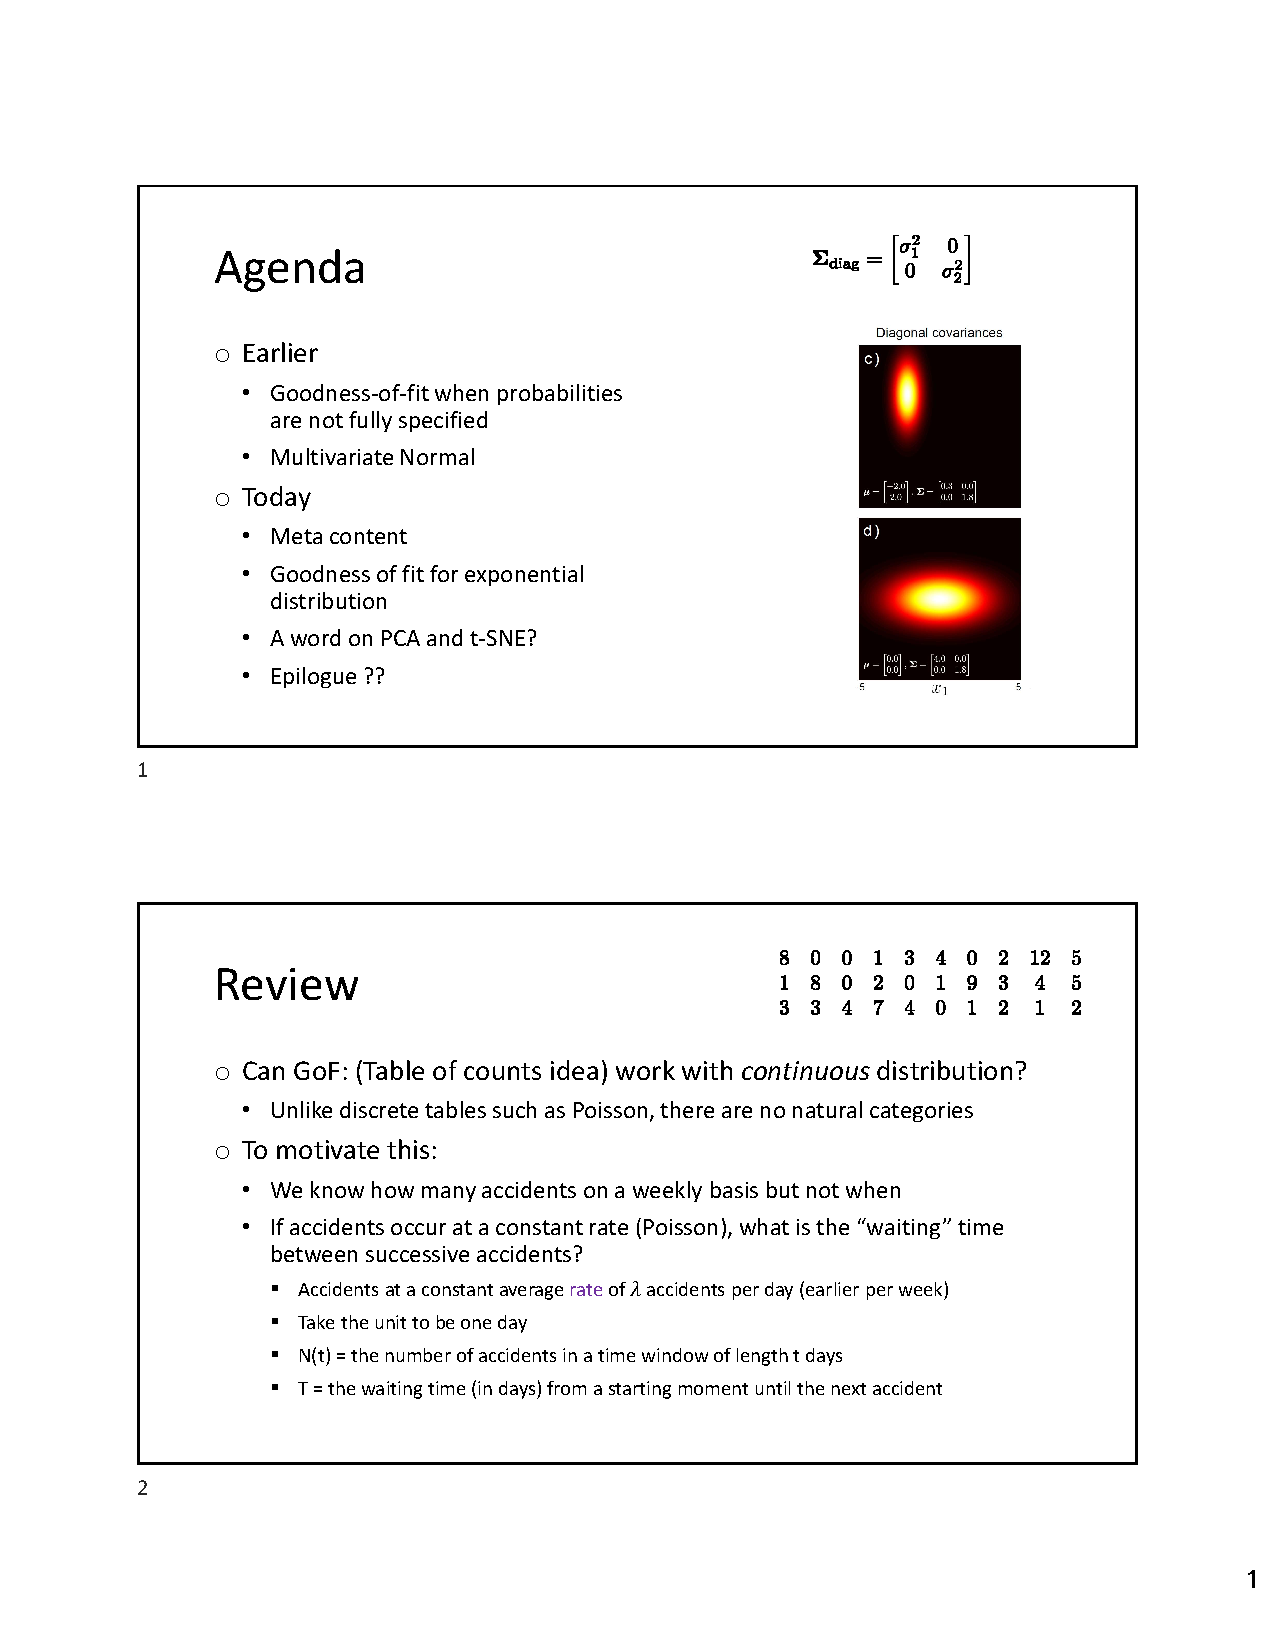
\includepdf[pages=-]{Lec44.pdf}
}

\subsection{PCA; t-SNE}
{
\setbeamercolor{background canvas}{bg=} 
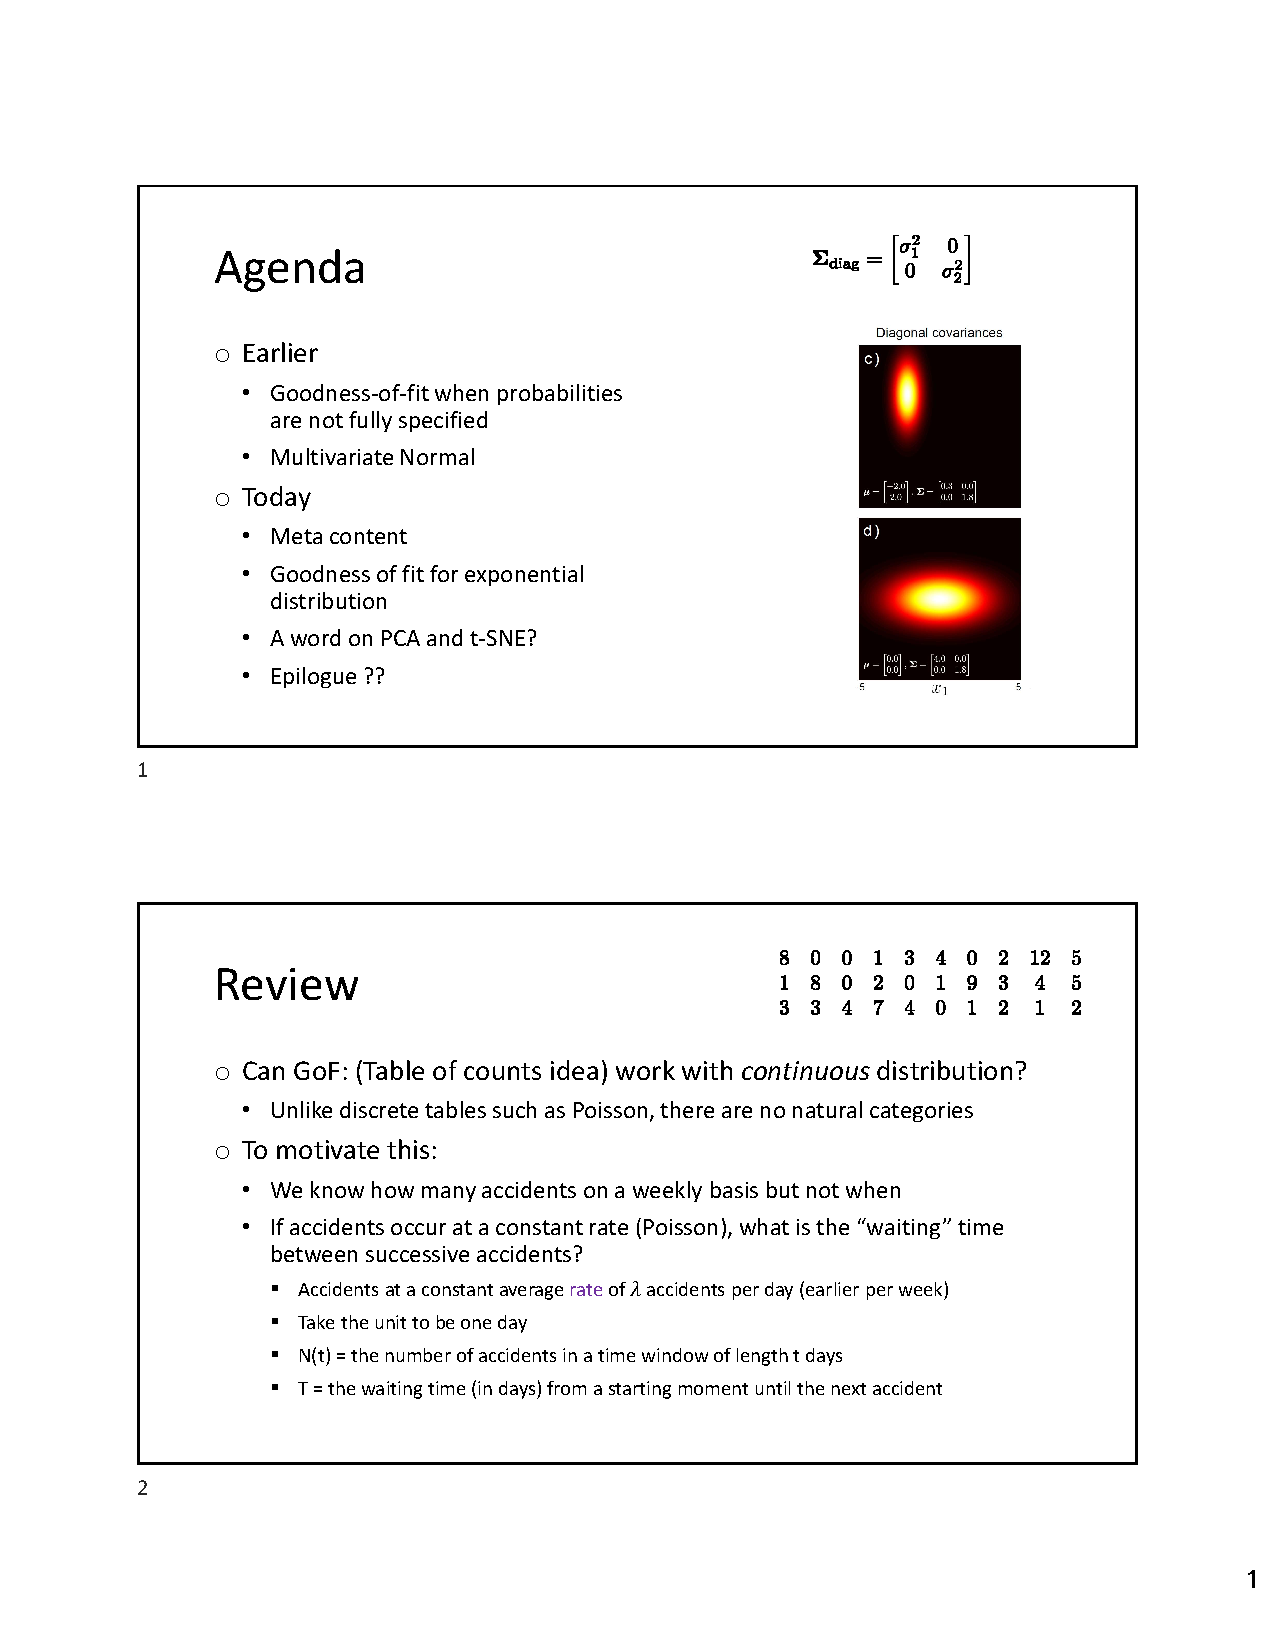
\includepdf[pages=-]{Lec45.pdf}
}

\section{Midsem Questions Review}
{
\setbeamercolor{background canvas}{bg=} 
\includepdf[pages=-]{Lec20.pdf}
\includepdf[pages=-]{Lec26.pdf}
\includepdf[pages=-]{Lec27.pdf}
}




\end{document}


